\documentclass[a4paper,twoside,11pt]{report}
\usepackage{hyperref}
\usepackage{caption}
\usepackage{appunti}
\usepackage{float}
\usepackage[english,italian]{babel}
\usepackage[utf8]{inputenc}
\usepackage[T1]{fontenc}
\usepackage{graphicx}
\usepackage[Conny]{fncychap}
\usepackage{amsmath}
\usepackage{amssymb}
\usepackage{wrapfig}
\usepackage[parfill]{parskip}
\usepackage{cases}

\usepackage{hyperref}
\hypersetup{
	colorlinks,
	citecolor=black,
	filecolor=black,
	linkcolor=red,
	urlcolor=black
}

\begin{document}

\titolo{Metodi ed algoritmi di ottimizzazione per il problem solving}
\candidato{Edoardo Rosa}
\relatore{Aristide Mingozzi}

\annoaccademico{20014-2015}

\copertinatesi
\indice
\indicefigure
\indicetabelle
\iniziatesto

\chapter{Modelli e formulazioni matematiche}

\section{The Traveling Salesman Problem}
Il Traveling Salesman Problem (TSP) è il problema più noto dell'ottimizzazione combinatoria.
Siano date $n$ città e i costi $c_{ij}$ per andare dalla città $i$ alla città $j$.
Si vuole determinare un cammino che parte da una città (diciamo $i_{1}$), visitare una ed una sola volta tutte le rimanenti città e terminare nella città di partenza $i_{1}$.
Inoltre si vuole che il costo di tale cammino sia minimo.\newline
Ha molteplici applicazioni pratiche e teoriche perche è la struttura di molti problemi pratici.\newline
Si è soliti modella il TSP come segue:
\begin{itemize}
	\item è dato un grafo orientato (o non orientato) $G = (N,A)$
	dove $N$ è un insieme di $n$ vertici e $A$ è un insieme di $m$ archi.
	
	Ad ogni arco $\emph{(i,j)} \in \emph{A}$ è associato un costo $c_{ij}$.
	
	Un circuito hamiltoniano di $G$ è un circuito che passa per ogni vertice una ed una sola volta.\newline
	Il costo di un circuito hamiltoniano di $G$ è pari alla somma dei costi degli archi che compongono il circuito;
	\item il problema del TSP è di trovare un grafo $G$, con una data matrice dei costi [$c_{ij}$], un circuito hamiltoniano di costo minimo.
\end{itemize}
\newpage
\subsection{Formulazioni Matematiche del TSP}
In letteratura esistono molteplici (e a volte fantasiose) formulazioni del TSP.\newline
Presentiamo le due formulazioni più note e su cui si basano i metodi esatti più efficienti.

\subsubsection{TSP asimmetrico}
I costi $c_{ij}$ non verificano $c_{ij} = c_{ji}\;\forall\;i,j$ con $i < j$.\newline
Sia $x_{ij}$ una variabile $(0-1)$ associata ad ogni arco $(i,j) \in A$ dove $x_{ij}=1$ se l'arco $(i,j)$ è nella soluzione ottima e $x_{ij}=0$ altrimenti.\newline

\begin{equation}
	Min\;\;\displaystyle\sum_{i\in N}^{} \sum_{j\in N}^{} c_{ij} x_{ij}
\end{equation}
\begin{equation}
	s.t.\;\;\displaystyle\sum_{i\in N}^{} x_{ij} = 1,\;\;\forall j \in N
\end{equation}
\begin{equation}
	\;\;\;\;\;\;\;\displaystyle\sum_{j\in N}^{} x_{ij} = 1,\;\;\forall i \in N
\end{equation}
\begin{equation}
	\;\;\;\;\;\;\;\;\;\;\;\;\;\;\;\;\;\;\displaystyle\sum_{i\in S}^{} \sum_{j\in N\setminus S}^{} x_{ij} \ge 1,\;\;\forall S \subset N
\end{equation}
\begin{equation}
	\;\;\;\;\;\;\;\;\;\;x_{ij} \in \{0,1\}\;,\;\forall (i,j) \in A
\end{equation}

Il vincolo $1.4$ impone che ogni soluzione ammissibile debba contenere almeno un arco $(i,j)$ con $i\in S$ e $j\in N\setminus S$ per ogni sottoinsieme $S$ di $N$.
Un'alternativa al vincolo $1.4$ è:
\begin{equation}\tag{1.4'}
\;\;\;\;\;\;\;\;\;\;\;\;\;\;\;\;\;\;\displaystyle\sum_{i\in S}^{} \sum_{j\in S}^{} x_{ij} \le |S| - 1,\;\;\forall S \subset N
\end{equation}

\subsubsection{TSP simmetrico}
Sia dato un grafo non-orientato $G=(N,A)$ con $c_{ij} = c_{ji}\:,\forall i,j\in N$.\newline
Gli archi di $A$ sono numerati da $1$ a $m$. L'arco di indice $l$ corrisponde a $(\alpha_{l},\beta_{l})$ con $\alpha_{l} < \beta_{l}$.\newline
$A_{i}$ è il sottoinsieme degli indici degli archi che incidono sul vertice $i$:
\begin{center}
	$A_{i} = \{l:\;l=1,m\;\;s.t.\;\alpha_{l}=i\;or\;\beta_{l}=i\}$
\end{center}

Per una dato $S\in N$ e $\bar{S} = N\setminus S$ indichiamo con $(S, \bar{S})$ il sottoinsieme degli indici degli archi per cui $\alpha_{l}\in S$ e $\beta_{l}\in \bar{S}$ oppure $\alpha_{l}\in \bar{S}$ e $\beta_{l}\in S$.

Ad ogni arco di incide $l$ è associato un costo $d_{l}=c_{\alpha_{l}\beta_{l}}$ e $x_{l}\in \{0,1\}$ è una variabile che vale 1 se e solo se l'arco di indice $l$ è nella soluzione ottima.
\begin{equation}
	Min\;\;\displaystyle\sum_{l=1}^{} d_{l}\:x_{l}
\end{equation}
\begin{equation}
	s.t.\;\;\displaystyle\sum_{l\in A_{i}}^{} x_{l}=2,\; \forall i\in N
\end{equation}
\begin{equation}
	\;\;\;\;\;\;\;\;\;\displaystyle\sum_{l\in (S, \bar{S})}^{} x_{l} \ge 1,\;\forall S \subset N
\end{equation}
\begin{equation}
	x_{l}\in \{0,1\},\;\;l=1,...,m
\end{equation}

\subsection{Eliminazione subtours di Miller, Tucker, Zemlin (1960)}
Sia $u_{i}$ una variabile intera il cui valore sappresenta la posizione che il vertice $i$ occupa nel tour.

\begin{center}
	Es. tour (1,4,5,3,2,1) per TSP con n=5 vertici, si ha $u_{1}=1,\;u_{2}=5,\;u_{3}=4,\;u_{4}=2,\;u_{5}=3$	
\end{center}

Miller, Tucker e Zemlin propongono in alternativa a:
\begin{equation}\tag{*}
	\displaystyle\sum_{i\in S}^{}\sum_{j\in N\setminus S}^{} x_{ij} \ge 1,\;\;\forall S\subset N
\end{equation}
hanno imposto i seguenti vincoli:
\begin{equation}
	u_{i}-u_{j}+nx_{ij}\le n-1,\;\; i=1,...,n\:,\;j=2,...,n
\end{equation}
Ogni tour hamiltoniano soddisfa questi vincoli e ogni subtour li viola.\newline
\begin{wrapfigure}[5]{l}{0.5\textwidth}
	\vspace{-2em}
	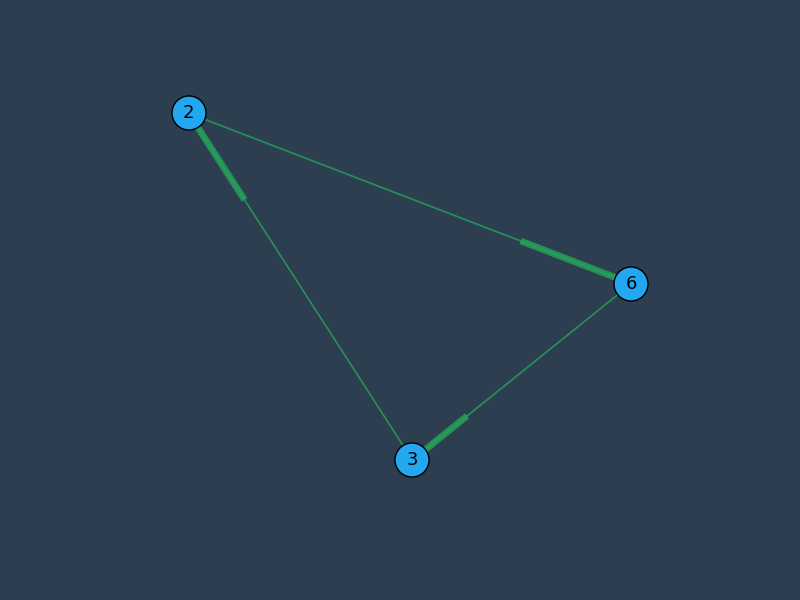
\includegraphics[height=5cm]{images/graph1.png}
	\caption{Grafo orientato}
\end{wrapfigure}
\begin{description}
	\vspace{1.5em}
	\item $u_{2}-u_{6}+n\;\cdot x_{2,6}\le n-1$
	\item $u_{6}-u_{3}+n\;\cdot x_{6,3}\le n-1$
	\item $u_{3}-u_{2}+n\;\cdot x_{3,2}\le n-1$
	\item {\hskip 5.6em}$\downarrow$
	\item {\hskip 3em}$3n \le 3(n-1)$
\end{description}\newpage

\subsection{Il Traveling salesman problem con time windows (TSPTW)}
È una variante del TSP che ha molte applicazioni.

Sia dato un grafo orientato $G=(V,A)$ di $n+1$ vertici $(V=\{0,1,...,n\})$.

Ad ogni arco $(i,j)\in A$ sono associati
\begin{itemize}
	\item un costo $c_{ij} \ge 0$
	\item un tempo di percorrenza $\theta_{ij}\ge 0$
\end{itemize}
Ad ogni vertice è associato un intervallo $[r_{i},d_{i}]$ chiamato "time window" che rappresenta l'orario in cui il vertice $i$ può essere vistato dal "salesman".

Ovvero il salesman può visitare $i$ ad ogni tempo $t\in \mathbb{Z}^{+}$ con $r_{i}\le t\le d_{i}$.\newline
Il problema consiste nel trovare una sequenza dei vertici di $G$ che parte dal vertice $0$ al tempo $0$ e finisce al nodo $0$ tale che sia il minimo il costo del circuito e il tempo di arrivo al nodo $i$ sia nell'intervallo $[r_{i},d_{j}],\;\forall i\in V$.\newline
Si consideri la sequenza $(0,i,..,i_{k-1},i_{k},...,i_{n},0)$ e sia $t_{i_{k}}$ il tempo di arrivo al vertice $i_{k},\; k=0,1,...,n+1$.

I tempi di arrivo sono calcolati come:
\begin{equation}
	t_{0}=0
\end{equation}
\begin{equation}
	t_{i_{k}}=\max \{t_{i_{k-1}}+\theta_{i_{k-1}}\cdot i_{k},\; r_{i_{k}}\}
\end{equation}

\subsubsection{Formulazione del TSPTW}
Sia $x_{ij}$ una variabile binaria intera che assume il valore $1$ se il vertice $i$ è visitato immediatamente prima di $i$ e $x_{ij}=0$ altrimenti.
\begin{flalign}
	& Min\;\;\displaystyle\sum_{(i,j)\in A}^{}c_{ik}x_{ij} \\
	& s.t.\;\;\;\;\displaystyle\sum_{i\in A_{j}^{-}}^{}x_{ij}=1,\;\;\forall j\in V \\		
	& \;\;\;\;\;\;\;\;\displaystyle\sum_{j\in A_{i}^{+}}^{}x_{ij}=1,\;\;\forall i\in V \\
	& \;\;\;\;\;\;\;\;t_{i}+\theta_{ij}-t_{j}\le M(1-x_{ij},\;\;\forall (i,j)\in A,\; j\ne 0) \\
	& \;\;\;\;\;\;\;\;t_{i}\le d_{i},\;\;\forall i\in V \\
	& \;\;\;\;\;\;\;\;t_{i}\ge r_{i},\;\;\forall i\in V \\
	& \;\;\;\;\;\;\;\;x_{ij}\in \{0,1\},\;\;\forall \in A \\
	& \;\;\;\;\;\;\;\;t_{i}\in \mathbb{N}^{+},\;\;\forall i\in V
\end{flalign}

dove 
\begin{flalign*}
	& A_{i}^{+}=\{j\in V:(i,j)\in A\} \\
	& A_{i}^{-}=\{j\in V:(i,j)\in A\} \\
	& M\;è\;un\;intero\;grande\;a\;piacere \\
	& r_{0}=d_{0}=0
\end{flalign*}
\newpage

\section{Project scheduling with resource constraints (PSR)}
\`E dato un insieme $\mathbb{X}=\{1,...,n\}$ di $n$ jobs.

Sono disponibili $m$ risorse dove ogni risorsa $k$ ha una disponibilità $b_{k}$ ad ogni istante del periodo di scheduling.

Ogni job $i$ ha un tempo di processo $d_{i}$ e la sua esecuzione, una volta iniziata, non può essere interrotta.

Il job $i$ per essere eseguito richiede $b_{ik}$ unità della risorsa $k$ per ciascun intervallo di tempo in cui rimane in esecuzione.\newline
\`E dato un grafo $G=(X,H)$ di precedenze, dove ogni arco $(i,j)\in H$ impone che il job $j$ può iniziare solo dopo che il job $i$ è stato completato.

\begin{itemize}
	\item Si vuole determinare il tempo di inizio di processo di ogni job in modo che siano soddisfatti i vincoli di precedenza, i vincoli sulle risorse e sia minima la durata complessiva del progetto
\end{itemize}

\subsection{Esempio di PSR}
Siano dati $n=11$ jobs e $m=3$ risorse con $b_{1}=b_{2}=b_{3}=4$ e un grafo $H$ delle precedenze corrispondenti agli archi della figura ~\ref{fig:grafoHDellePrecedenze}.

Si osservi che i jobs $2$ e $3$ non possono essere eseguiti in parallelo poiché $r_{2,1}+r_{3,1}=5 > b_{1}$!

\begin{figure}[h]
	\caption{Grafo H delle precedenze}
	\centering
	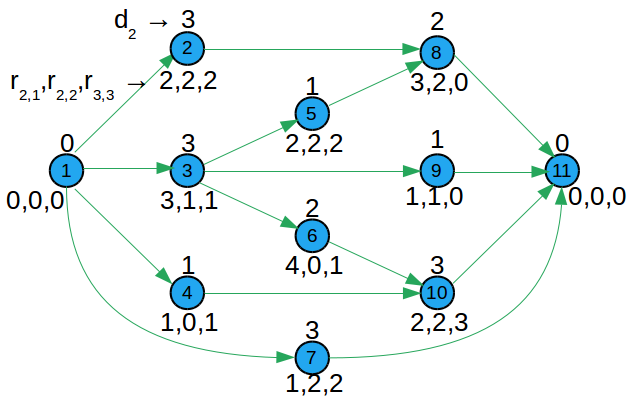
\includegraphics[height=6.5cm]{images/graph2.png}
	\label{fig:grafoHDellePrecedenze}
\end{figure}

\subsection{Formulazione del PSR}
Sia $\xi_{it}$ una variabile binaria 0-1 che vale 1 se e solo se il job $i$ viene messo in esecuzione al tempo $t$.

Sia $T_{max}$ un upper bound sulla durata del progetto.

\begin{flalign}
	& Min \displaystyle\sum_{t=1}^{T_{max}}t\;\xi_{n t} \\
	& \;\;s.t. \displaystyle\sum_{t=1}^{T_{max}}t\;\xi_{i t} = 1,\;\;\;i=1,...,n \\
	& \;\;\;\;\;\;\;\displaystyle\sum_{t=1}^{T_{max}}t\;\xi_{j t} - \displaystyle\sum_{t=1}^{T_{max}}t\;\xi_{i t} \ge d_{i},\;\;\;\forall (i,j)\in H \\
	& \;\;\;\;\;\;\;\displaystyle\sum_{i=1}^{n}r_{ik}\displaystyle\sum_{\tau=t-d_{i}+1}^{t}\xi_{i\tau}\le b_{k},\;\;\;t=1,...,T_{max}\;e\;k=1,...,m \\
	& \;\;\;\;\;\;\;\;\;\;\;\;\;\;\;\;\;\;\;\;\;\;\;\;\;\;
	\;\;\;\;\;\;\xi_{it}\in\{0,1\},\;\;\; i=1,...,n\;e\;t=1,...,T_{max}
\end{flalign}
Si osservi che:
\begin{flalign*}
	& \displaystyle\sum_{\tau=t-d_{i}+1}^{t}\xi_{i \tau}=1\;\;\;se\;il\;job\;i\;è\;in\;esecuzione\;al\;tempo\;t
\end{flalign*}
\subsubsection{Esempio}
Sia $d_{i}=4$.

Se $\xi_{i3}=1$, allora i è in esecuzione nei tempi 3,4,5 e 6.
Infatti avremo: \newline $\displaystyle\sum_{\tau=t-d_{i}+1}^{t}\xi_{i \tau} = 1$ per $t=3,4,5,6\;$ e $\displaystyle\sum_{\tau=t-d_{i}+1}^{t}\xi_{i \tau} = 0$ per $t<3$ e $t>6$
\newpage
\section{Fixed Charge Transportation Problem (FCTP)}
Il Problema del Trasporto di Carico Fisso è una generalizzazione del classico Problema del Trasporto.

Si differenzia nel definire che il costo per la spedizione di una quantità non-zero di beni, da ogni origine alla sua destinazione, è composto da un costo proporzionale all'ammontare dei beni inviati più un costo fisso. 

\subsection{Descrizione del FCTP}
Il FCTP è definito su un grafo completo e bipartito $G=(S,T,A)$ dove $S={1,2,...,m}$ è un insieme di $m$ sorgenti e $T={1,2,...,n}$ è un insieme di $n$ destinazioni.

Per ogni sorgente $i\in S$ è disponibile è una quantità intera $a_{i}>0$ di merce e per ogni destinazione $j\in T$ è necessaria una quantità intera $b_{j}>0$ di merce dalle sorgenti.\newline
L'insieme $A$ degli archi è definito come: $A=\{(i,j):\;i\in S,\;j\in T\}$; ogni arco $(i,j)\in A$ è
associato ad un costo unitario $c_{ij}$ per il trasporto di una unità della merce dalla sorgente $i$ alla destinazione $j$ più un costo fisso $f_{ij}$ for usare l'arco $(i,j)$.

Senza perdere di generalità si assume che:
\begin{flalign*}
	& \displaystyle\sum_{i\in S}^{}a_{i}=\displaystyle\sum_{j\in T}^{}b_{j} \\
\end{flalign*}

\subsection{Formulazione del FCTP}
Sia $x_{ij}$ una variabile rappresentante la quantità di merce trasportata dalla sorgente $i$ alla destinazione $j$ e $y_{ij}$ una variabile (0-1) che vale $1$ se e solo se $x_{ij}>0$.

Sia $m_{ij}=min{a_{i},b_{j},\;(i,j)\in A}$.\newline
Una semplice formulazione matematiche del FCTP è:
\begin{flalign}
	& z(F0) = min \displaystyle\sum_{i\in S}^{}\displaystyle\sum_{j\in T}^{}(c_{ij}x_{ij}+f_{ij}y_{ij}) \\
	\label{con:1.27}
	& \;\;\;\;\;\;\;s.t.\;\;\displaystyle\sum_{j\in T}^{}x_{ij}=a_{i},\;\;i\in S \\
	\label{con:1.28}
	& \;\;\;\;\;\;\;\;\;\;\;\;\;\;\displaystyle\sum_{i\in S}^{}x_{ij} = b_{j},\;\;j\in T \\
	& \;\;\;\;\;\;\;\;\;\;\;\;\;\;x_{ij}\le m_{ij}y_{ij},\;\;\;(i,j)\in A \\
	& \;\;\;\;\;\;\;\;\;\;\;\;\;\;x_{ij}\ge 0,\;\;\;\;\;\;\;\;\;\;\;(i,j)\in A \\
	& \;\;\;\;\;\;\;\;\;\;\;\;\;\;y_{ij}\in \{0,1\}
\end{flalign}
Si denota con $LF0$ il rilassamento lineare del problema $F0$ e con $z(LF0)$ il costo della soluzione ottima. Notare che, per ogni soluzione ottima di $LF0$, le variabili $x_{ij}>0$ corrispondono ad una soluzione base fattibile dei vincoli \ref{con:1.27} e \ref{con:1.28}, e $y_{ij}=x_{ij}/m_{ij}\;con\;(i,j)\in A$.
\newpage
\section{Assegnamento dei veicoli alle baie di carico}
Sia dato un insieme $N$ di veicoli che devono scaricare presso un deposito che ha un insieme $L$ di linee di scarico.

Per ogni linea di scarico $j\in L$ è definito l'insieme degli istanti di tempo $T_{j}$ in cui è operativa.\newline
Per ogni veicolo $i\in N$ sono noti:
\begin{itemize}
	\item il sottoinsieme di linee $L_{i}\subseteq L$ compatibili con le operazioni di scarico richieste dal veicolo;
	\item iltempo di arrivo $a_{i}$ del veicolo al deposito;
	\item la durata dello scarico $d_{ij}$ sulla linea $j\in L_{i}$.
\end{itemize}
Si assume che lo scarico di un veicolo non possa essere interrotto, ovvero, se lo scarico del veicolo $i$ sulla linea $j\in L_{i}$ inizia al tempo $t$, allora la linea $j$ deve essere disponibile per tutti gli istanti di tempo $\tau=t,...,t+d_{ij}-1$ (ovvero $\tau \in T_{j}$ per ogni $\tau=t,...,t+d_{ij}-1$).
Indichiamo con $I_{ij}$ l'insieme degli istanti di tempo in cui può iniziare lo scarico del veicolo $i$ sulla linea $j\in L_{i}$, ovvero per ogni $t\in I_{ij}$ si assume che la linea $j$ disponibile per ogni istante $\tau=i,...,d_{ij}-1$.

Sia $c_{ijt}$ è il costo per iniziare lo scarico del veicolo $i\in N$ sulla linea $j\in L{i}$ al tempo $t\in I_{ij}$.\newline
Il problema richiede che ogni veicolo sia assegnato ad una linea di scarico compatibile in modo che ogni scarico sia fatto senza interruzioni e sia minimo il costo dell'assegnamento.

\subsection{Formulazione matematica F}
Per ogni $i\in N$, $j\in L_{i}$ e $t\in I_{ij}$ poniamo $\delta_{ijt\tau}=1$ per $\tau=t,...,t+d_{ij}-1$ e $\delta_{ijt\tau}=0$ per ogni $\tau\in T_{j}$ tale che $\tau < t$ oppure $\tau >t+d_{ij}-1$.

Indichiamo con $N_{j}\subseteq N$ il sottoinsieme di veicoli che possono essere scaricati sulla linea $j$, ovvero $N_{j}=\{i\in N:\;j\in L_{i}\}$.

\subsubsection{Variabili}
$x_{ijt}$ è una variabile (0-1) che vale 1 se e solo se il veicolo $i\in N$ inizia lo scarico sulla linea $j\in L_{i}$ al tempo $t\in I_{ij}$.

$s_{j\tau}$ è una variabile (0-1) che vale 1 se e solo se la linea $j$ non viene utilizzata nell'istante di tempo $\tau$.\newline
La formulazione matematica $F$ del problema è la seguente.
\begin{flalign}
	& z(F)=min\sum_{j\in L}^{}\sum_{i\in N_{j}}^{}\sum_{t\in I_{ij}}^{}c_{ijt}+x_{ijt}+\sum_{j\in L}^{}\sum_{\tau\in T_{j}}^{}g_{j\tau}s_{j\tau} \\
	\label{con:1.33}
	& \;\;\;\;\;\;\;\;s.t.\;\;\sum_{j\in L_{i}}^{}\sum_{t\in I_{ij}}^{}x_{ijt}=1,\;\;\;i\in N \\
	\label{con:1.34}
	& \;\;\;\;\;\;\;\;\;\;\;\;\;\;
	\sum_{i\in N_{j}}^{}\sum_{t\in I_{ij}}^{}\delta_{ijt\tau}x_{ijt}+s_{j\tau}=1,\;\;\;j\in L,\;\tau\in T_{j} \\
	& \;\;\;\;\;\;\;\;\;\;\;\;\;\; 
	x_{ijt}\in {0,1},\;\;\;\;\;\;\;\;\;\;\;\;\;\;
	i\in N,\;j\in L_{i},\;t\in I_{ij} \\
	& \;\;\;\;\;\;\;\;\;\;\;\;\;\; 
	s_{j\tau}\in {0,1},\;\;\;\;\;\;\;\;\;\;\;\;\;\;
	j\in L,\;\tau\in T_{j}
\end{flalign}
Il vincolo \ref{con:1.33} impone che ad ogni veicolo venga assegnato una linea compatibile ed un tempo di scarico a sua volta compatibile sia con il veicolo stesso che con la linea a lui assegnata.

Il vincolo \ref{con:1.34} impone che per ogni linea ed ogni istante di tempo compatibile con la linea vi sia in scarico al più un solo veicolo.\newline
La formulazione $F$ richiede $\hat{n}=|N|\times|L|\times\hat{I}$ variabili, dove $\hat{I}=max{|I_{ij}|:i\in N,\;j\in L_{i}}$ e al più $\hat{m}=|N|+|L|\times \hat{T}$ vincoli, dove $\hat{T}=max{|T_{j}|:\;j\in L}$.

Supponiamo di discretizzare il tempo a 5 minuti, che ogni linea sia disponibile al più 10 ore (i.e. $\hat{T}=120$) e che un veicolo quando arriva non possa aspettare più di 5 ore (i.e. $\hat{I}=60$). Avremo $\hat{n}=200\cdot20\cdot60=240.000$ e $\hat{m}=200+20\cdot120=2600$.
\newpage

\section{Lot Sizing Problem}
Il termine \textit{\textbf{Lot Sizing}} indica il processo decisionale mediante il quale un'azienda definisce la politica ottima di investimenti, produzione e stoccaggio dei prodotti per soddisfare le richieste dei clienti nel rispetto dei vincoli di produzione e di magazzino.

Non esiste un unico modello di lot sizing che rappresenti in modo generale le varie realtà operative. Sistemi di produzione anche marginalmente diversi possono richiedere modelli aventi complessità computazionale molto diverse.

Non esiste in letteratura un modello generale che contenga come sottocasi tutti i problemi reali noti di lot sizing.

Per questi motivi non esistono software commerciali general pourpose.\newline
Diverse aziende di consulenze nel settore della supply chain vendono software basati su modelli semplificati che non necessariamente producono soluzioni operative ma lasciano all'utente il compito di modificare manualmente la soluzione prodotta per tener conto delle specifiche complessità del problema reale.\newline
I problemi reali sono varianti complesse delle seguenti tre classi di lot sizing problem di un singolo prodotto che sono risolvibili in tempo polinomiale:
\begin{itemize}
	\item lot sizing senza vincoli di capacità produttiva;
	\item lot sizing con back logging senza vincoli di capacità;
	\item lot sizing con vincoli di capacità.
\end{itemize}
Molti problemi reali possono essere risolti rilassando in modo lagrangiano i vincoli reali per cui il problema lagrangiano risultante corrisponde ad uno dei tre problemi suddetti.

\subsection{Lot sizing senza vincoli di capacit\`a}
Si consideri un'azienda che deve pianificare la propria produzione per un orizzonte temporale di $T$ periodi (ad esempio, $T$ mesi).

Per ciascun periodo $t=1,...,T$ sono noti:
\begin{itemize}
	\item[\textit{$d_{t}$}] domanda complessiva dei clienti;
	\item[\textit{$A_{t}$}] costo fisso di set up per attivare la produzione;
	\item[\textit{$p_{t}$}] costo per produrre un'unità di prodotto;
	\item[\textit{$h_{t}$}] costo per unità di prodotto presente nel magazzino alla fine del periodo $t$. 
\end{itemize}
Per ciascun periodo $t$, deve essere deciso il numero di unità che devono essere prodotto al fine di soddisfare la domanda in ciascun periodo.\newline
Si suppone che la quantità prodotto nel periodo $t$ sia subito disponibile e che la quantità non venduta alla fine di ogni mese viene depositata in magazzino.
L'obiettivo è di minimizzare i costi complessivi di set up, produzione e stoccaggio.

\subsubsection{Formulazione Matematica (modello di Wagner-Whitin)}
Variabili decisonali associate a ciascun periodo t=1,...,T
\begin{description}
	\item[$x_{t}$] quantità prodotta all'inizio del periodo $t$;
	\item[$I_{t}$] livello del magazzino alla fine del periodo $t$;
	\item[$y_{i}\in (0,1): y_{t}=1$] se nel periodo $t$ vi è produzione, $y_{t}=0$ altrimenti. 
\end{description}

\begin{flalign}
	& Min\;z=\sum_{t=1}^{T} (p_{t}x_{t}+h_{t}I_{t}+A_{t}y_{t}) \\
	&\;\;\;\;\;\;\;\;x_{t}+I_{t-1}=I_{t}+d_{t},\;t=1,...,T \\
	& \;\;\;\;\;\;\;\;x_{t}\le My_{t},\;t=1,..., \\
	& \;\;\;\;\;\;\;\;x_{t},\;I_{t}\ge 0,\;t=1,...,T \\
	& \;\;\;\;\;\;\;\;y_{t}\in \{0,1\},\;t=1,...,T \\
	& dove\;M=\sum_{t=1}^{T}d_{t}\;e,\;per\;semplicità,\;si;suppone\;che\;I_{0}=0.
\end{flalign}

\subsubsection{Metodo di soluzione}
Al modello si associa il grafo $R=(N,A)$ senza vincoli di capacità sugli archi tale che ogni soluzione del problema corrisponde ad un flusso in $R$.\newline
Il grafo $R$ si compone di $2T+1$ nodi:
\begin{itemize}
	\item nodo sorgente S da cui parte un flusso pari a $\sum_{t=1}^{T}d_{t}$;
	\item per ciascun periodo $t$ una coppia di nodi $U_{t}$, $V_{t}$ dove:
	\begin{itemize}
		\item[$U_{t}$] rappresenta il magazzino,
		\item[$V_{t}$] corrisponde alla domanda.
	\end{itemize}
\end{itemize}
Per ciascun periodo $t=1,..,T$ vi sono gli archi:
\begin{description}
	\item[$(S,U_{t})$] ~~~~il cui flusso corrisponde alla produzione $x_{t}$;
	\item[$(U_{t},U_{t+1})$] il cui flusso è pari al livello $I_{t}$ del magazzino alla fine del periodo $t$;
	\item[$(U_{t},V_{t})$] ~~~~il cui flusso deve essere pari alla domanda $d_{t}$.
\end{description}
\newpage
\begin{figure}
	\caption{Esempio della rete di flusso (modello di Wagner-Whitin)}
	\centering
	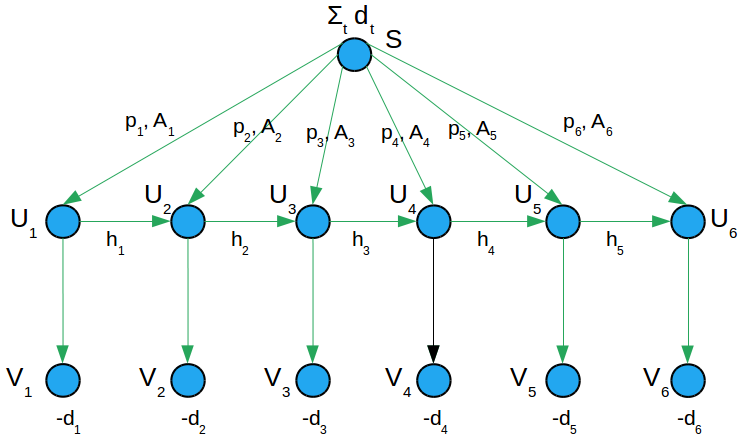
\includegraphics[height=8.5cm]{images/graph3.png}
	\label{fig:WagnerWhitin}
\end{figure}

\subsubsection{Proprietà della soluzione ottima}
\textbf{Teorema.} In una soluzione ottima non può mai avvenire che la domanda del periodo $t$ venga soddisfatta sia dalla produzione che dal magazzino, ovvero:
\begin{center}
	$I_{t-1}\cdot x_{t}=0;\;t=1,...,T$
\end{center}
\begin{figure}[H]
	\caption{}
	\centering
	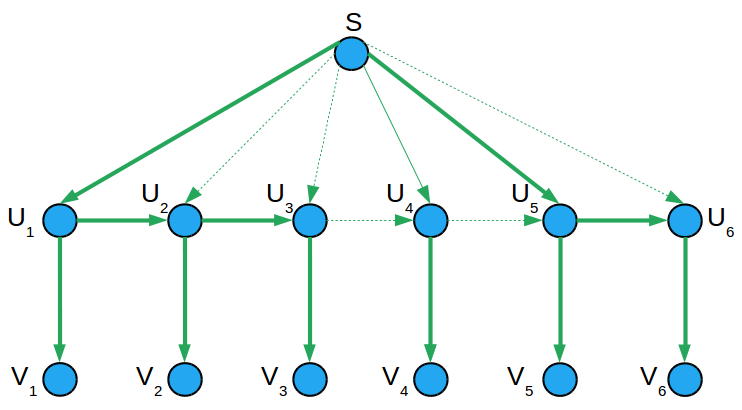
\includegraphics[height=5.6cm]{images/graph4.png}
	\label{fig:PossibileSoluzione}
\end{figure}

\subsubsection{Algoritmo di soluzione (di complessità $O(T^{2})$)}
Si costruisca un grafo aciclico di $T+1$ vertici.\newline
Si definiscano gli archi $j,k)$ per $j=0,...,T-1$ e $k=j+1,...,T$.

L'arco $(j,k)$ rappresenta la decisione di produrre all'inizio del periodo $j+1$ quanto serve per soddisfare le domanda complessiva dei periodo $j+1,\;j+2,...,k$.

Il costo $M_{jk}$ dell'arco (j,k) è pari al costo per produrre nel periodo j+1 la quantità $\sum_{r=j+1}^{k}d_{r}$ più i costi di stoccaggio:
\begin{center}
	$M_{jk}=A_{j+1}+p_{j+1}\displaystyle\sum_{r=j+1}^{k}d_{r}+\sum_{t=j+1}^{k-1}h_{t}(\sum_{r=t+1}^{k}d_{r})$
\end{center}
\begin{figure}[H]
	\caption{}
	\centering
	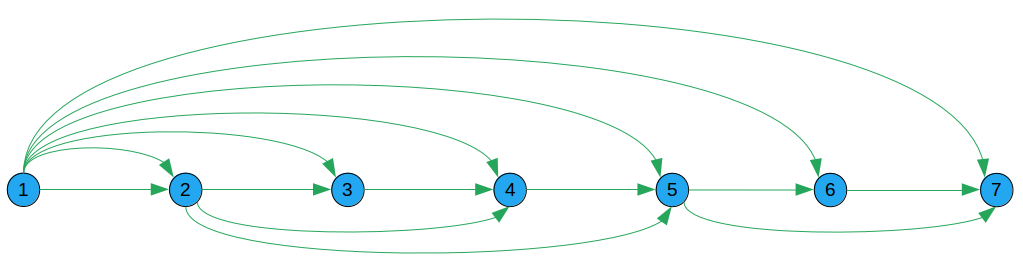
\includegraphics[height=4.2cm]{images/graph5.png}
	\label{fig:PossibileSoluzione2}
\end{figure}

Ogni soluzione del modello di Wagner-Whitin corrisponde ad un cammino da $0$ a $t$ in questo grafo aciclico.\newline
Il cammino di costo minimo fornisce la soluzione ottima.
\chapter{Introduzione alla programmazione lineare a numeri interi}

\section{}
\chapter{Rilassamento Lagrangiano per il calcolo di lower bounds}
Si consideri il seguente problema $P$ di programmazione a numeri interi:
\begin{displaymath}
P:
\begin{cases}
	z(P)=Min\;cx \\
	\;\;\;\;\;\;\;\;\;\;\;\;s.t.\;Ax\ge b \\
	\;\;\;\;\;\;\;\;\;\;\;\;\;\;\;\;\;\;Bx\ge d \\
	\;\;\;\;\;\;\;\;\;\;\;\;\;\;\;\;\;\;x\in\{0,1\}^{n} 
\end{cases}
\end{displaymath}
Il valore ottimo $z(LP)$ del rilassamento lineare $LP$ del problema $P$ fornisce un valido lower bound, ovvero
\begin{equation}
	z(LP)\le z(P)
\end{equation}
$LP$ si ottiene da $P$ sostituendo $x\in\{0,1\}^{n}$ con $0\le x\le 1$:
\begin{displaymath}
LP:
\begin{cases}
z(LP)=Min\;cx \\
\;\;\;\;\;\;\;\;\;\;\;\;\;\;\;s.t.\;Ax\ge b \\
\;\;\;\;\;\;\;\;\;\;\;\;\;\;\;\;\;\;\;\;\;Bx\ge d \\
\;\;\;\;\;\;\;\;\;\;\;\;\;\;\;\;\;\;\;\;\;0\le x\le 1
\end{cases}
\end{displaymath}
In molti casi:
\begin{itemize}
	\item è pribitivo risolvere $LP$: troppe variabili e/o vincoli;
	\item $z(LP)$ è troppo distante da $z(P)$ e quindi non utilizzabile in un algoritmo Branch and Bound.
\end{itemize}

\section{Rilassamento Lagrangiano di $P$ rispetto ai vincoli $Ax\ge b$}
Viene così definito il problema $RL_{u}$ che si ottiene da $P$ rimuovendo i vincoli $Ax\ge b$ e sottraendo dalla funzione obiettivo il termine $u(Ax-b)$ dove $u\ge 0$ è il vettore dei \textbf{Moltiplicatori Lagrangiani}.
\begin{displaymath}
	RL_{u}:
	\begin{cases}
		L(u)=Min\;cx-u(Ax-b) \\
		\;\;\;\;\;\;\;\;\;\;\;\;s.t.\;Bx\ge d \\
		\;\;\;\;\;\;\;\;\;\;\;\;\;\;\;\;\;\;x\in\{0,1\}
	\end{cases}
\end{displaymath}
$L(u)$ viene detta "\textit{Funzione Lagrangiana}"

\subsection{Esempio}
\begin{displaymath}
P:
\begin{cases}
z(P)=Min\;3x_{1}+7x_{2}+10x_{3} \\
\;\;\;\;\;\;\;\;\;\;\;\;s.t.\;x_{1}+3x_{2}+5x_{3}\ge 7 \\
\;\;\;\;\;\;\;\;\;\;\;\;\;\;\;\;\;\;x_{1},x_{2},x_{3}\in\{0,1\}
\end{cases}
\end{displaymath}
\begin{displaymath}
RL_{u}:
\begin{cases}
L(u)=Min\;x_{1}+7x_{2}+10x{3}-u(x_{1}+3x_{2}+5x_{3}-7) \\
\;\;\;\;\;\;\;\;\;\;\;\;s.t.\;x_{1},x_{2},x_{3}\in\{0,1\}
\end{cases}
\end{displaymath}

\section{Validità e importanza di $RL_{u}$}
Possiamo dimostrare che $L(u)\le z(P),\;\forall u\ge0$ e quindi $\underset{u\ge 0}{Max}[L(u)]\le z(P)$.\\
In certe condizioni la soluzione ottima di $RL_{u}$ è anche la soluzione ottima di $P$.

\subsection{Esempio}
\begin{displaymath}
P:
\begin{cases}
z(P)=Min\;2x_{1}+3x_{2}+4x_{3}+5x_{4} \\
\;\;\;\;\;\;\;\;\;\;\;\;s.t.\;x_{1}+x_{3}\ge 1 \\
\;\;\;\;\;\;\;\;\;\;\;\;\;\;\;\;\;\;x_{1}+x_{4}\ge 1 \\
\;\;\;\;\;\;\;\;\;\;\;\;\;\;\;\;\;\;x_{2}+x_{3}+x_{4}\ge 1 \\
\;\;\;\;\;\;\;\;\;\;\;\;\;\;\;\;\;\;\forall i \in \{0,1\},\;i=1,\dots,4 \\
\end{cases}
\end{displaymath}
La soluzione ottima è $x_{1}=x_{2}=1,\;x_{3}=x_{4}=0$ e $z(P)=S$.\\
Il rilassamento lagrangiano dei tre vincoli richiede tre moltiplicatori $u_{1},u_{2},u_{3}$; quindi
\begin{flalign}
	& (RL_{u})\;\;\;\;L(u))=Min\;2x_{1}+3x_{2}+4x_{3}+5x_{4} -u_{1}(x_{1}+x_{3}-1) \\
	& \;\;\;\;\;\;\;\;\;\;\;\;\;\;\;\;\;\;\;\;\;\;\;\;\;\;\;\;\;\;\;\;\;\;\;\;\;\;\;\;\;\;\;\;\;\;\;\;\;\;\;\;\;\;\;\;\;\;\;\;\;\;\;\;\;\;\;\;\;\;\;-u_{2}(x_{1}+x_{4}-1) \\
	& \;\;\;\;\;\;\;\;\;\;\;\;\;\;\;\;\;\;\;\;\;\;\;\;\;\;\;\;\;\;\;\;\;\;\;\;\;\;\;\;\;\;\;\;\;\;\;\;\;\;\;\;\;\;\;\;\;\;\;\;\;\;\;\;\;\;\;\;\;\;\;-u_{3}(x_{2}+x_{3}+x_{4}-1 ) \\
	&\;\;\;\;\;\;\;\;\;\;\;\;\;\;\;\;\;\;\;\;\;s.t.\; x_{i}\in\{0,1\},\;i=1,\dots,4
\end{flalign}
ma anche
\begin{flalign}
	& (RL_{u})\;L(u)=Min\;(2-u_{1}-u_{2})x_{1}+(3-u_{3})x_{2}+(4-u_{1}-u_{3})x_{3}+(5-u_{2}-u_{3})x_{4}+u_{1}+u_{2}+u_{3} \\
	& \;\;\;\;\;\;\;\;\;\;\;\;\;\;\;\;\;\;\;\;\;\;s.t.\;x_{i}\in\{0,1\},\;i=1,\dots,4
\end{flalign}
Dato $u$, la soluzione ottima di $RL_{u}$ e, conseguentemente, il valore di $L(u)$ si ottiene ponendo
\begin{flalign*}
	& x_{i}=0\textnormal{ se il coefficiente di $x_{i}$ è }\ge 0 \\
	& x_{i}=1\textnormal{ se il coefficiente di $x_{i}$ è }< 0 \\
\end{flalign*}
Poniamo $u_{1}=1.5$, $u_{2}=1.6$ e $u_{3})=2.2$
\begin{equation*}
	L(u)=Min\; -1.1x_{1}+0.8x_{2}+0.3x_{3}+1.2x_{4}+1.5+1.6+2.2
\end{equation*}
La soluzione ottima è
\begin{equation*}
	x_{1}=1,\;x_{2}=x_{3}=x_{4}=0
\end{equation*}
quindi
\begin{equation*}
	L(u)=-1.1+1.5+1.6+2.2=5.3-1.1=4.2
\end{equation*}
Ponendo $u_{1}=1$, $u_{2}=1$ e $u_{3}=3$
\begin{equation*}
L(u)=Min\; 0x_{1}+0x_{2}+0x_{3}+x_{4}+1+1+3
\end{equation*}
Una soluzione ottima è
\begin{equation*}
x_{1}=1=x_{2}=x_{3}=x_{4}=0
\end{equation*}
di costo $L(u)=0+0+0+0+1+1+3=5\equiv z(P)$.\\
Si noti che esistono soluzioni ottime alternative tutte di costo $L(u)$=5 che si ottengono ponendo $x_{1}=1$ e/o $x_{2}=1$ e/o $x_{3}=1$ e $x_{4}=0$. Fra tali soluzioni esiste quella ottima! $x_{1}=x_{2}=1$ e $x_{3}=x_{4}=0$

\section{TEOREMA: Dualità Lagrangiana debole}
Il valore ottimo $z(P)$ del problema
\begin{displaymath}
P:
\begin{cases}
z(P)=Min\;\;cx \\
\;\;\;\;\;\;\;\;\;\;\;\;s.t.\;Ax\ge b \\
\;\;\;\;\;\;\;\;\;\;\;\;\;\;\;\;\;\;Bx\ge d \\
\;\;\;\;\;\;\;\;\;\;\;\;\;\;\;\;\;\;x\in \{0,1\} \\
\end{cases}
\end{displaymath}
è maggiore o uguale al valore ottimo $L(u)$ del problema
\begin{displaymath}
RL_{u}:
\begin{cases}
L(u)=Min\;cx-u(Ax-b) \\
\;\;\;\;\;\;\;\;\;\;\;\;s.t.\;Bx\ge d \\
\;\;\;\;\;\;\;\;\;\;\;\;\;\;\;\;\;\;x\in \{0,1\} \\
\;\;\;\;\;\;\;\;\;\;\;\;\;\;\;\;\;\;\forall u\ge 0 \\
\end{cases}
\end{displaymath}
\subsection{Dimostrazione}
Sia $x^{*}$ la soluzione ottima di $P$. Si noti che $x^{*}$ è anche una soluzione ammissibile per $RL_{u}$ per ogni $u\ge 0$, ma non necessariamente l'ottimo di $RL_{u}$ per un dato $u$.\\
Si ha, quindi, che
\begin{equation}
	cx^{*}-u(Ax^{*}-b)\ge L(u)
\end{equation}
ma $u(Ax^{*}-b)\ge 0$ (poichè $u\ge 0$ e $Ax^{*}\ge b$ essendo per ipotesi $x^{*}$ l'ottimo di $P$); quindi
\begin{equation}
	cx^{*}\ge L(u)\textnormal{ ovvero }z(P)\ge L(u)\;\;\;\;\;\;\;\;\;\;\square
\end{equation}

\section{Lagrangiano Duale}
Dal teorema della dualità debole per cui $L(u)\le z(P)$, $\forall u\ge 0$, si ha che l'ottimo $z(D_{L})$ del seguente problema:
\begin{equation}
	D_{L}\;\;\;\;\;\;z(D_{L})=\underset{u\ge 0}{Max}\;[L(u)]
\end{equation}
è un valido lower bound a $z(P)$; ovvero $z(D_{L})\le z(P)$.\\
Il problema $D_{L}$ è detto \textit{Lagrangiano Duale} di $P$.

\section{Duality Gap}
Nel caso in cui $z(D_{L})<z(P)$ allora si dice che esiste un \textbf{duality gap} fra il problema $P$ e il problema $D_{L}$.\\
Supponiamo che l'ottimo di $D_{L}$ si ottenga risolvendo $L(\bar{u})$ per un dato $\bar{u}\ge 0$, ovvero, $z(D_{L})=L(\bar{u})$.\\
Indichiamo con $\bar{x}$ la soluzione ottima di $RL_{\bar{u}}$ ovvero:
\begin{equation}
	z(D_{L})=L(\bar{u})=c\bar{x}-\bar{u}(A\bar{x}-b)
\end{equation}
Si consideri il caso in cui $\bar{x}$ è anche l'ottimo di $P$, ovvero, $z(P)=c\bar{x}$.\\\\
È evidente che $z(D_{L})<z(P)$ se $\bar{u}(A\bar{x}-b)>0$.

\subsection{Esempio}
\begin{displaymath}
P:
\begin{cases}
z(P)=Min\;3_x{1}+7x_{2}+10x_{3} \\
\;\;\;\;\;\;\;\;\;\;\;\;s.t.\;x_{1}+3x_{2}+5x_{3}\ge 7 \\
\end{cases}
\end{displaymath}
\begin{equation*}
	L(u)=Min\;3x_{1}+7x_{2}+10x_{3}-u(x_{1}+3x_{2}+5x_{3}-7)
\end{equation*}
\begin{equation*}
	x_{1},x_{2},x_{3}\in \{0,1\}
\end{equation*}
Per calcolare $z(D_{L})\underset{u\ge 0}{Max}[L(u)]$ calcoliamo $L(u)$, $u\ge 0$
\begin{flalign*}
	& u=0\;\;\;\;\;\;L(0)=0\;\;\;\;\;\;\;\;\;\;\;\;\;\;\;\;\;x=(0,0,0) \\
	& u=1\;\;\;\;\;\;L(1)=7\;\;\;\;\;\;\;\;\;\;\;\;\;\;\;\;\;x=(0,0,0) \\
	& u=2\;\;\;\;\;\;L(2)=14\;\;\;\;\;\;\;\;\;\;\;\;\;\;\;x=(0,0,0)\textnormal{ oppure }x=(0,0,1) \\
	& u=\frac{7}{3}\;\;\;\;\;L(\frac{7}{3})=\frac{44}{3}\;\;\;\;\;\;\;\;\;\;\;\;\;\;x=(0,0,1)\textnormal{ oppure }x=(0,1,1) \\
	& u=3\;\;\;\;\;\;L(3)=14\;\;\;\;\;\;\;\;\;\;\;\;\;\;\;\;x=(0,1,1)\textnormal{ oppure }x=(1,1,1) \\
	& u>3\;\;\;\;\;\;L(u)=-2u+20\;\;\;\;\;x=(1,1,1) \\
\end{flalign*}
Quindi $z(D_{L})=\frac{44}{3}$ mentre $z(P)=17$ e $x^{*}=(0,1,1)$ che corrisponde ad una delle soluzioni di $L(\frac{7}{3})=\frac{44}{3}$ ma esiste un gap di dualità.

\section{TEOREMA: Dualità Lagrangiana Forte}
Sia $\bar{x}$ la soluzione ottima di $L(u)$, per un dato $\bar{x}\ge 0$.\\
Se $\bar{x}$, $\bar{u}$ soddisfano le seguenti condizioni:
\begin{flalign}
	A\bar{x}\ge b \label{eq:3.12}\\
	\bar{u}(A\bar{x}-b)=0 \label{eq:3.13}
\end{flalign}
allora $\bar{x}$ è la soluzione ottima di $P$ ed inoltre $z(D_{L})=L(\bar{u})=z(P)$.
\subsection{Dimostrazione}
Dimostraimo che se $\bar{x}$, $\bar{u}$ soddisfano le \ref{eq:3.12} e \ref{eq:3.13} allora $\bar{x}$ è una soluzione ottima di $P$.\\
Poichè $\bar{x}$ soddisfa la \ref{eq:3.12} allora è soluzione ammissibile di $P$ e quindi
\begin{equation}
	\label{eq:3.14}
	c\bar{x}\ge z(P)
\end{equation}
Per il teorema della dualità Lagrangiana debole si ha:
\begin{equation}
	\label{eq:3.15}
	z(P)\ge L(u)=c\bar{x}-\underbrace{\bar{u}(A\bar{x}-b)}_{=0 \textnormal{ per la \ref{eq:3.13}}}
\end{equation}
Quindi da \ref{eq:3.14} e \ref{eq:3.15} si ottiene
\begin{equation}
	c\bar{x}\ge z(P)\ge c\bar{x}\textnormal{ ovvero }z(P)=c\bar{x}.
\end{equation}
Dimostriamo che se $\bar{x}$ e $\bar{u}$ soddisfano le \ref{eq:3.12} e \ref{eq:3.13} allora $z(D_{L})=L(\bar{u})=z(P)$.\\
Per come è definito il problema $D_{L}$ si ha che:
\begin{flalign*}
	& z(D_{L})\ge L(\bar{u}) \\
	& z(P)\ge z(D_{L}) \numberthis\label{eq:3.17}
\end{flalign*}
Abbiamo dimostrato che se valgono \ref{eq:3.12} e \ref{eq:3.13} allora
\begin{equation}
	\label{eq:3.18}
	z(P)=L(\bar{u})=c\bar{x}
\end{equation}
Quindi da \ref{eq:3.17} e \ref{eq:3.18} si ottiene
\begin{equation}
	z(D_{L})=z(P)
\end{equation}
$\square$

\subsection{Osservazioni}
\begin{itemize}
	\item Qual è il migliore sottoinsieme di vincoli da rilassare in modo Lagrangiano?
	\item Come risolvere $D_{L}$: ovvero come scegliere i valori numerici di $u$ in modo da ottenere il miglior possibile lower bound.
	\item Che relazione esiste tra $z(D_{L})$ e $z(LP)$ il valore del Rilassamento Lineare di $P$?
\end{itemize}

\section{Caratterizzazione del Lagrangiano Duale}
Al fine di stabilire una relazione tra $D_{L}$ ed il rilassamento lineare $LP$ di $P$ è utile riformulare $D_{L}$ come un problema di programmazione lineare.
\subsection{Definizione}
Indichiamo $X=\{x: Bx\ge d,\;x\in(0,1) \}$ e con $conv(X)$ l'invilupopo convesso di tutti i punti di $X$ (ovvero, $conv(X)$ è l'intersezione di tutti gli insieme convessi che contengono $X$).
\centerline{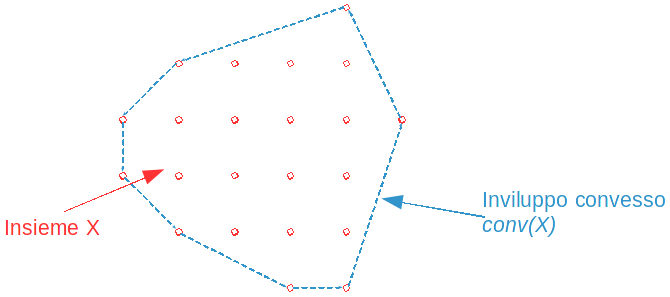
\includegraphics[height=4.5cm]{images/graph27.png}}
Si osservi che l'ottimo del problema Lagrangiano:
\begin{displaymath}
	RL_{u}
	\begin{cases}
		L(u)=Min\;cx-u(Ax-b) \\
		\;\;\;\;\;\;\;\;\;\;\;\;\;\;\;\;\;\;\;\;s.t.\;Bx\ge d \\
		\;\;\;\;\;\;\;\;\;\;\;\;\;\;\;\;\;\;\;\;\;\;\;\;\;\;x\in (0,1)
	\end{cases}
\end{displaymath}
corrisponde ad un punto estremo di $conv(X)$
\subsection{TEOREMA}
Il Lagrangiano Duale $D_{L}$ corrisponde al seguente problema di programmazione lineare.
\begin{displaymath}
D_{L}
\begin{cases}
z(D_{L})=Min\;cx \\
\;\;\;\;\;\;\;\;\;\;\;\;\;\;\;\;\;\;\;\;s.t.\;Ax\ge d \\
\;\;\;\;\;\;\;\;\;\;\;\;\;\;\;\;\;\;\;\;\;\;\;\;\;\;x\in conv(X)
\end{cases}
\end{displaymath}
dove $X=\{x:Bx\ge d,\;x\in(0,1)\}$ e $conv(X)$ è l'inviluppo convesso di $X$.
\subsubsection{Dimostrazione}
Si ricordi che:
\begin{equation*}
	D_{L}\;\;\;\;\;z(D_{L})=\underset{u\ge 0}{Max}\;[L(u)]
\end{equation*}
e, per come è stato definite $X$, il problema $RL_{u}$ diviene
\begin{equation*}
	RL_{u}\;\;\;\;\;L(u)=\underset{x\in X}{Min}\;(cx-u(Ax-b))
\end{equation*}
Quindi, il problema $D_{L}$ può essere scritto come:
\begin{equation*}
	D_{L}\;\;\;\;\;z(D_{L})=\underset{u\ge 0}{Max}\;[\underbrace{\underset{x\in X}{Min)}\;(cx-u(Ax-b))]}_{L(u)}
\end{equation*}
o anche
\begin{equation*}
D_{L}\;\;\;\;\;z(D_{L})=\underset{u\ge 0}{Max}\;[\underset{x\in conv(X)}{Min)}\;(cx-u(Ax-b))]
\end{equation*}
poichè $L(u)$ raggiunge l'ottimo in un punto estremo di $conv(X)$.\\
Indichiamo con $x^{i},\;i=1,\dots,t$ i punti estremi di $conv(X)$. Il problema $D_{L}$ può essere scritto come:
\begin{equation*}
	D_{L}\;\;\;\;\;z(D_{L})=\underset{u\ge 0}{Max}\;[\underset{1\le i\ge t}{Min}\;(cx^{i}-u(Ax^{i}-b))]
\end{equation*}
quest'ultimo problema può essere riformulato mediante la programmazione lineare come segue:
\begin{equation*}
	D_{L}
	\begin{cases}
	z(D_{L})=Max\; v \\
	\;\;\;\;\;\;\;\;\;\;\;\;\;\;\;s.t.\; v\le cx^{i}-u(Ax^{i}-b),\;i=1,\dots,t\\
	\;\;\;\;\;\;\;\;\;\;\;\;\;\;\;\;\;\;\;\;\;\textnormal{v qualsiasi} \\
	\;\;\;\;\;\;\;\;\;\;\;\;\;\;\;\;\;\;\;\;\;u\ge 0
	\end{cases}
\end{equation*}
Il duale di questo problema è il seguente
\begin{equation*}
	DD_{L}
	\begin{cases}
		z(D_{L})=Min\;\sum_{i=1}^{t}\lambda_{i}(cx^{i})\\
		\;\;\;\;\;\;\;\;\;\;\;\;\;\;\;s.t.\; \sum_{i=1}^{t}\lambda_{i}=1 \\
		\;\;\;\;\;\;\;\;\;\;\;\;\;\;\;\;\;\;\;\;\;\sum_{i=1}^{t}\lambda_{i}(Ax^{i}-b)\ge 0 \\
		\;\;\;\;\;\;\;\;\;\;\;\;\;\;\;\;\;\;\;\;\;\lambda_{i}\ge 0,\;i=1,\dots,t
	\end{cases}
\end{equation*}
Si noti che $\sum_{i=1}^{t}\lambda_{i}(cx^{i})=c(\sum_{i=1}^{t}\lambda_{i}x^{i})$ ed inoltre $\sum_{i=1}^{t}=\lambda_{i}(Ax^{i}-b)=A(\sum_{i=1}^{t}\lambda_{i}x^{i})-b(\sum_{i=1}^{t}\lambda_{i})$.\\
Quindi $DD_{L}$ può essere riscritto come
\begin{numcases}{DD_{L}}
	z(D_{L})=Min\;c(\sum_{i=1}^{t}\lambda_{i}x^{i}) \\
	\;\;\;\;\;\;\;\;\;\;\;\;\;\;s.t.\;\sum_{i=1}^{t}\lambda_{i}=1 \label{eq:3.21}\\
	\;\;\;\;\;\;\;\;\;\;\;\;\;\;\;\;\;\;\;\;A(\sum_{i=1}^{t}\lambda_{i}x^{i})\ge b(\sum_{i=1}^{t}\lambda_{i}) \label{eq:3.22}\\
	\;\;\;\;\;\;\;\;\;\;\;\;\;\;\;\;\;\;\;\;\lambda_{i}\ge 0,\;i=1,\dots,t \label{eq:3.23}
\end{numcases}
Si osservi che, per ognu t-pla $\lambda_{i},\dots,\lambda_{t}$ che soddisfa i vincoli \ref*{eq:3.21} e \ref{eq:3.23}, il punto $x=\sum_{i=1}^{t}\lambda_{i}x^{i}$ appartiene a $conv(X)$. Quindi il problema $DD_{L}$ può essere riscritto come
\begin{equation}
	DD_{L}
	\begin{cases}
		z(D_{L})=Min\;cx \\
		\;\;\;\;\;\;\;\;\;\;\;\;\;\;s.t.\;Ax\ge b \\
		\;\;\;\;\;\;\;\;\;\;\;\;\;\;\;\;\;\;\;\;x\in conv(X)
	\end{cases}
\end{equation}
$\square$

\section{Lagrangiano Duale e Rilassamento Lineare}
\subsection{TEOREMA}
\begin{equation}
	z(D_{L})\ge z(LP)
\end{equation}
\subsection{Dimostrazione}
Il rilassamento lineare $LP$ è definito come
\begin{equation}
	LP
	\begin{cases}
		z(LP)=Min\;cx \\
		\;\;\;\;\;\;\;\;\;\;\;\;\;\;\;s.t.\;Ax\ge b \\
		\;\;\;\;\;\;\;\;\;\;\;\;\;\;\;\;\;\;\;\;\;Bx\ge d \\
		\;\;\;\;\;\;\;\;\;\;\;\;\;\;\;\;\;\;\;\;\;0\le x\le 1
	\end{cases}
\end{equation}
Definiamo $\bar{X}=\{x:Bx\ge d,\;0\le x\le 1\}$, quindi
\begin{equation}
	LP
	\begin{cases}
		z(LP)=Min\;cx \\
		\;\;\;\;\;\;\;\;\;\;\;\;\;\;\;s.t.\;Ax\ge b\\
		\;\;\;\;\;\;\;\;\;\;\;\;\;\;\;\;\;\;\;\;\;x\in\bar{X}
	\end{cases}
\end{equation}
Per come abbiamo definito $\bar{X}$ è facile osservare che:
\begin{equation}
	conv(X)\subseteq\bar{X}
\end{equation}
e poichè abbiamo dimostrato che
\begin{equation}
	D_{L}
	\begin{cases}
		z(D_{L})=Min\;cx\\
		\;\;\;\;\;\;\;\;\;\;\;\;\;\;\;s.t.\;Ax\ge b \\
		\;\;\;\;\;\;\;\;\;\;\;\;\;\;\;\;\;\;\;\;\;x\in conv(X)
	\end{cases}
\end{equation}
si ha che $z(D_{L})\ge z(LP)$.\\
$\square$

\subsection{TEOREMA: $\boldsymbol{L(u)}$ è concava}
La funzione lagrangiana $L(u)$ è concava, ovvero $L(\lambda u^{1}+(1-\lambda)u^{2})\ge \lambda L(u^{1})+(1-\lambda)L(u^{2})$, $\lambda \in [0,1]$

\centerline{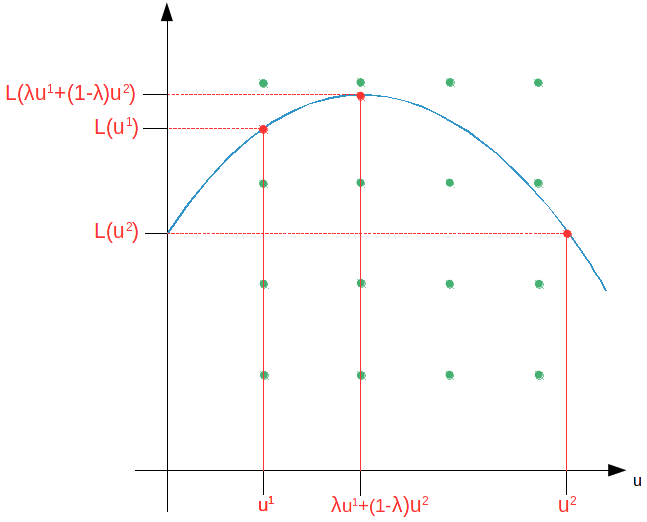
\includegraphics[height=8cm]{images/graph28.png}}

\subsubsection{Dimostrazione}
Siano $u^{1},u^{2}\ge 0$ e $u^{0}=\lambda u^{1}+(1-\lambda)u^{2}$ con $\lambda in[0,1]$.\\
Indichiamo con $x^{0}$ la soluzione ottima di $RL_{u^{0}}$:
\begin{equation}
	L(u^{0})=cx^{0}-u^{0}(Ax^{0}-b)
\end{equation}
$x^{0}$ è soluzione ammissibile di $RL_{u^{1}}$ e $RL_{u^{2}}$ quindi
\begin{flalign}
	L(u^{1})\le cx^{0}-u^{1}(Ax^{0}-b) \label{eq:3.31} \\
	L(u^{2})\ge cx^{0}-u^{2}(Ax^{0}-b) \label{eq:3.32}
\end{flalign}
Moltiplicando la \ref{eq:3.31} per $\lambda$, la \ref{eq:3.32} e sommando:
\begin{equation}
	\lambda L(u^{1})+(1-\lambda)L(u^{2})\le cx^{0}-\underbrace{(\lambda u^{1}+(1-\lambda)u^{2})}_{u^{0}}(Ax^{0}-b)=L(u^{0})
\end{equation}

\section{Subgradiente di $\boldsymbol{L(u)}$}
Un vettore è detto subgradiente di $L(u)$ in $\bar{u}$ se soddisfa
\begin{equation}
	L(u)\ge L(\bar{u})+y(u-\bar{u})
\end{equation}

\centerline{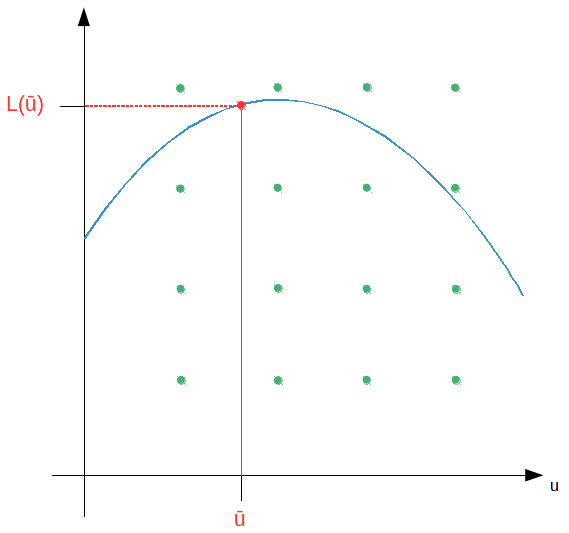
\includegraphics[height=7cm]{images/graph29.png}}

\textbf{Come calcolare $\boldsymbol{y}$?}\\
Sia $\bar{x}$ tale che
\begin{equation}
	L(\bar{u})=c\bar{x}-\bar{u}(A\bar{x}-b) \label{eq:3.35}
\end{equation}
Per ogni $u\ge 0$ si ha
\begin{equation}
	L(u)\le c\bar{x}-u(A\bar{x}-b) \label{eq:3.36}
\end{equation}
Sottraendo dalla \ref{eq:3.36} la \ref{eq:3.35} si ottiene
\begin{equation}
	L(u)=L(\bar{u})\ge -(A\bar{x}-b)(u-\bar{u})
\end{equation}
ma anche
\begin{equation}
	L(u)\le L(\bar{u})-(A\bar{x}-b)(u-\bar{u})
\end{equation}
ne segue che $y=-(A\bar{x}-b)$ è un subgradiente di $L(u)$ in $\bar{u}$

\subsection{Metodo del subgradiente}
Metodo iterativo per risolvere il lagrangiano duale
\begin{equation*}
	D_{L}
	\begin{cases}
		z(D_{L})=\underset{u\ge 0}{Max}[L(u)]
	\end{cases}
\end{equation*}
Il metodo genera una sequenza finita di punti $(u^{1},u^{2},\dots,u^{k})$ e, quindi, calcola
\begin{equation*}
	z(D_{L})=\underset{u\in \{u^{1},u^{2},\dots,u^{k}\}}{Max}[L(u)]
\end{equation*}
\subsubsection{Generazione di $\boldsymbol{u^{r}}$ in funzione di $\boldsymbol{u^{r-1}}$}
Sia $x^{r-1}$ tale che $L(u^{r-1})=cx^{r-1}-u^{r-1}(Ax^{r-1}-b)$.\\
Abbiamo dimostrato che
\begin{equation}
	L(u^{r})\le L(u^{r-1})-(Ax^{r-1}-b)(u^{r}-u^{r-1})
\end{equation}
se vogliamo che $L(u^{r})$ possa essere maggiore di $L(u^{r-1})$ è necessario che
\begin{equation}
	-(Ax^{r-1}-b)(u^{r}-u^{r-1})>0 \label{eq:3.40}
\end{equation}
Si noti che una scelta di $u^{r}$ che verifichi la suddetta condizione non è sufficiente per garantire che $L(u^{r})>L(u^{r-1})$.\\
Come definire $u^{r}$ affinchè \ref{eq:3.40} sia verificata?\\
Supponiamo che $A$ abbia $m$ righe e quindi $u=(u_{1},\dots,u_{m})$ indicando con $a^{i}\ge b_{i}$ la i-esima disequazione di $Ax\ge b$; la condizione \ref{eq:3.40} può essere scritta come
\begin{equation*}
	-\sum_{i=1}^{m}(a_{i}^{r-1}-b_{i})(u_{i}^{r}-u_{i}^{r-1})>0 \label{eq:3.40bis}
\end{equation*}
Per soddisfare \ref{eq:3.40bis} è sufficiente determinare ogni $u_{i}^{r}$ in modo che
\begin{equation}
	-(a^{i}x^{r-1}-b_{i})(u_{i}^{r}-u_{i}^{r-1})>0,\;\forall i=1,\dots,m
\end{equation}
Da cui seguono i sequenti casi:

\begin{itemize}
	\item $a^{i}x^{r-1}$: $x^{r-1}$ viola il vincolo i-esimo \\
	definisci $u_{i}^{r}>u_{i}^{r-1}$
	\item $a^{i}x^{r-1}>b_{i}$: $x^{r-1}$ soddisfa il vincolo i-esimo \\
	definisci $u_{i}^{r}<u_{r}^{r-1}$ ma imponi $u_{i}^{r}\ge 0$
	\item $a^{i}x^{r-1}=b_{i}$: $x^{r-1}$ satura il vincolo i-esimo \\
	$u_{i}^{r}$ qualsiasi (è buona norma $u_{i}^{r}=u_{i}^{r-1}$!)
\end{itemize}

\begin{enumerate}
	\item Inizializza $u^{1}=0$ e poni $r=1$ e $LB=-\infty$
	\item Risolvi:
	\begin{equation*}
		L(u^{r})
		\begin{cases}
			Min\;cx-u^{r}(Ax-b)\\
			s.t.;Bx\ge d\\
			x\in(0,1)
		\end{cases}
	\end{equation*}
	Sia $x^{r}$ la soluzione ottima\\
	Se $L(u^{r})>LB$ allora poni $LB=L(u^{r})$ e $u^{*}=u^{r}$\\
	Se $Ax^{r}\ge b$ e $u^{r}(Ax^{r}-b)=0$ allora $x^{r}$ è soluzione ottima di $P$: STOP
	\item Definisci i moltiplicatori di $u^{r+1}$
	\begin{equation*}
		u_{i}^{r+1}=Max[0,\;u_{i}^{r}-\alpha \cdot\frac{z_{UB}-L(u^{r})}{\sum_{i=1}^{m}\widetilde{y_{i}^{2}}}\cdot\widetilde{y_{i}}],\;\forall i
	\end{equation*}
	dove $\widetilde{y_{i}}=a^{i}x^{r}-b_{i}$ e $\alpha$ è una costante ($0<\alpha\le 2$).\\
	Poni $r\gets r+1$ e ritorna allo step \textit{2}.
	\item Il metodo potrebbe non arrestarsi: è quindi necessario imporre un numero massimo di iterazioni.
	\item È opportuno diminuire il valore di $\alpha$ ($\alpha\gets\alpha/2$) se per $\delta$ iterazioni consecutive $L(u)\le LB$
	\item I valori di $\alpha$ e $\delta$ vanno determinati sperimentalmente: tipicamente $\alpha=2$ e $\delta=30$.
\end{enumerate}

\subsection{Vincoli Misti}
\begin{equation*}
	z(P)
	\begin{cases}
		Min\;cx\\
		\;\;\;\;\;\;\;\;A_{1}x\ge b_{1}\;\;\;\;m_{1}\textnormal{ righe e }u^{1}\ge 0 \\
		\;\;\;\;\;\;\;\;A_{2}x=b_{2}\;\;\;\;m_{2}\textnormal{ righe e }u^{2}\in \mathbb{R}^{m_{2}} \\
		\;\;\;\;\;\;\;\;A_{3}x\le b_{3}\;\;\;\;m_{3}\textnormal{ righe e }u^{3}\le 0 \\
		\;\;\;\;\;\;\;\;Bx\ge d \\
		\;\;\;\;\;\;\;\;\;\;\;x\in\{0,1\}^{m}\;\;\;\;\;\;\;\;\;\;\;\;\;\;\;u=(u^{1},u^{2},u^{3})
	\end{cases}
\end{equation*}
\begin{equation*}
	L(u)
	\begin{cases}
		Min\;cx-u^{1}(A_{1}x-b_{1})-u^{2}(A_{2}x-b_{2})-u^{3}(A_{3}x-b_{3})\\
		\;\;\;\;\;\;\;\;s.t.\;Bx\ge d\\
		\;\;\;\;\;\;\;\;\;\;\;\;\;\;\;\;\;x\in\{0,1\}^{m}
	\end{cases}
\end{equation*}
ma anche:
\begin{equation*}
	L(u)
	\begin{cases}
		Min\;(c-u^{1}A_{1}-u^{2}A_{2}-u^{3}A_{3})x+u^{1}b_{1}+u^{2}b_{2}+u^{3}b_{3}\\
		\;\;\;\;\;\;\;\;\;\;\;\;s.t.\;Bx\ge d \\
		\;\;\;\;\;\;\;\;\;\;\;\;\;\;\;\;\;\;\;\;\;x\in\{0,1\}
	\end{cases}
\end{equation*}

\subsection{Subgradiente per vincoli mist}
Ad una generica iterazione.\\
Sia $\bar{x}$ la soluzione ottima di $L(u)$.\\
Calcola $y^{1}=A_{1}\bar{x}-b_{1}$, $y^{2}=A_{2}\bar{x}-b_{2}$, $y^{3}=A_{3}\bar{x}-b_{3}$.\\
Poni $y=(y^{1},y^{2},y^{3})$ e $t=\alpha\frac{z_{UB}-L(u)}{\displaystyle\sum_{i=1}^{m}y_{1}^{2}}$
\begin{flalign*}
	& u_{i}^{1}\gets max[0,\;u_{i}^{1}-ty_{i}^{1}],\;i=1,\dots,m_{1}\\
	& u_{i}^{2}\gets u_{i}^{2}-ty_{i}^{2},\;i=1,\dots,m_{2}\\
	& u_{i}^{3}\gets min[0,\;u_{i}^{3}-ty_{i}^{3}],\;i=1,\dots,m_{3}
\end{flalign*}

\section{Traveling Salesman Problem}
\subsection{Costi Simmetrici}
$n$ vertici, $m$ archi.\\
$G=(N,A)$: grafo non-orientato.\\
$N=\{1,\dots,n\}$ insieme dei vertici.\\
$A=\{1,\dots,m\}$ insieme degli archi. \\
\textbf{Costi simmetrici:} $c_{ij}=c_{ji}$ $\forall\;ij$
Indichiamo con $c_{l}$ il costo dell'arco $l\in A$.\\
Per ogni arco $l\in A$ siano $(\alpha_{l},\beta_{l})$ i due vertici terminali.\\
Inoltre sia $B_{i}\subset A$ l'insieme degli archi incidenti nel vertice $i\in N$.
\subsubsection{Esempio}
\begin{minipage}[l]{0.5\textwidth}
	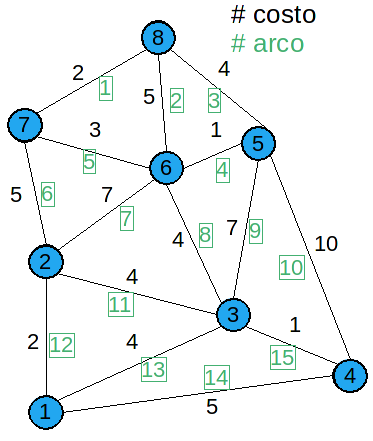
\includegraphics[height=7cm]{images/graph30.png}
\end{minipage}
\begin{minipage}[r]{0.5\textwidth}
	$n=8$ vertici\\
	$m=15$ archi\\04
	arco $14$ $\alpha_{14}=1$, $\beta_{14}=4$\\
	$B_{4}=\{10,14,15\}$\\
	$B_{3}=\{8,9,15,13,11\}$
\end{minipage}
\subsection{Fomulazione Matematica (TSP Simmetrico)}
$x_{l}=1$, se l'arco $l$ è nella soluzione ottima\\
$x_{l}=0$, altrimenti.
\begin{numcases}{}
Min\;z=\sum_{l=1}^{m}c_{l}x_{l}\\
\;\;\;\;\;\;\;\;\;\;\;\;\;\;\sum_{l\in B_{i}}x_{l}=2;\;i=1,\dots,n \label{eq:3.43}\\
\;\;\;\;\;\;\;\;\;\;\;\;\;\;\sum_{l\in K_{t}}x_{l}\ge 1;\; \forall K_{t}=(S_{t},\;N\setminus S_{t})\;\;\;\;S_{t}\subset N,\;S_{t}\neq\emptyset,\; |S_{t}|\ge 2 \label{eq:3.44}\\
\;\;\;\;\;\;\;\;\;\;\;\;\;\;x_{l}\in\{0,1\};\;l=1,\dots,m
\end{numcases}

\subsubsection{$\boldsymbol{1^{o}}$ Rilassamento Lagrangiano (SST)}
I vincoli \ref{eq:3.43} vengono portati nella fuzione obiettivo e sostituiti nella formulazione con il "surrogato" $\sum_{i=1}^{n}=(\sum_{l\in B_{i}}x_{l})=2n$.
\begin{flalign}
& L(\lambda)=min\;\sum_{l=1}^{m}c_{l}x_{l}-\sum_{i=1}^{n}\lambda_{i}(\sum_{l\in B_{i}}x_{l}-2)\\
& \sum_{l=1}^{m}x_{l}=n \label{eq:3.47} \\
& \sum_{l\in K_{t}}x_{l}\ge 1;\;\;\forall K_{t}=(S_{t},\;N\setminus S_{t})\;\;\;\;S_{t}\subset N,\;S_{t}\neq\emptyset \label{eq:3.49} \\
& x_{l}\in\{0,1\}\;\;l=1,\dots,m
\end{flalign}
\begin{flalign*}
& L(\lambda)=min\sum_{l=1}^{m}c_{l}x_{l}-\sum_{i=1}^{n}\lambda_{i}(\sum_{l\in B_{i}}x_{l}-2) \\
& L(\lambda)=min\sum_{l=1}^{m}c_{l}x_{l}+2\sum_{i=1}^{n}\lambda_{i}-\sum_{i=1}^{n}\sum_{l\in B_{i}}\lambda_{i}x_{l}
\end{flalign*}
Si noti che l'arco $l$ ha come vertici terminali $\alpha_{l}$, $\beta_{l}$ e quindi compare per $i=\alpha_{l}$ ed $i=\beta_{l}$.
\begin{flalign*}
& \sum_{i=1}^{n}\sum_{l\in B_{i}}\lambda_{i}x_{l}=\sum_{l=1}^{m}(\lambda+\lambda)x_{l} \\
& L(\lambda)=min\;\sum_{l=1}^{m}(\underbrace{c_{l}-\lambda_{\alpha_{l}}-\lambda_{\beta_{l}}}_{c'_{l}})x_{l}+2\sum_{i=1}^{n}\lambda_{i} \\
& \sum_{l=1}^{m}x_{l}=n \\
& \sum_{l\in K_{t}}x_{l}\ge 1;\;\;\;\forall K_{t}\equiv(S_{t},\;N\setminus S_{t})\;\;\;\;\;S_{t}\subset N,\;S_{t}\neq\emptyset \\
& x_{l}\in\{0,1\}
\end{flalign*}
La soluzione ottima si ottiene calcolando l'albero di costo minimo, usando i costi $(c_{l}-\lambda_{\alpha_{l}}-\lambda_{\beta_{l}})$, detto $v(SST)$ tale costo si ha che
\begin{equation}
	L(\lambda)=v(SST)+c'_{l_{min}}+2\sum_{i=1}^{n}\lambda_{i}
\end{equation}
dove $c_{l_{min}}'=min\{(c_{l}-\lambda_{\alpha_{l}}-\lambda_{\beta_{l}}):\;l\notin SST\}$

\subsection{Calcolo di $\boldsymbol{L(\lambda^{0})}$ per $\boldsymbol{\lambda^{0}=0}$}
\centerline{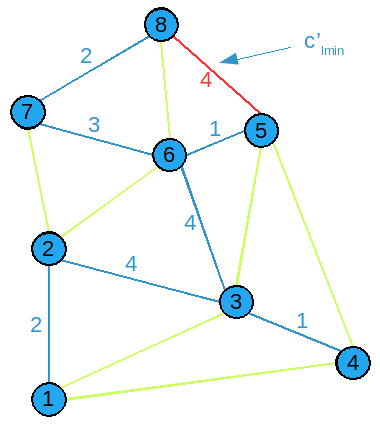
\includegraphics[height=7cm]{images/graph31.png}}
L'albero di costo minimo è $SST=\{(3,4),(6,5),(1,2),(7,8),(7,6),(2,3),(3,6)\}$ mentre l'arco minimo è $(5,8)$ e $c'_{l_{min}}=4$
\begin{equation}
	L(\lambda^{0})=v(SST)+c'_{l_{min}}=17+4=21
\end{equation}

\subsection{Calcolo Penalità Lagrangiane}
Poniamo $d_{i}=\sum_{l\in B_{i}}x_{l}$ per cui il vincolo
\begin{equation}
	\sum_{l\in B_{i}}x_{l}=2;\;\;\;\;i=1,\dots,n
\end{equation}
diviene
\begin{equation}
	d_{i}=2;\;\;\;\;i=1,\dots,n
\end{equation}
Nella soluzione prodotta per $\lambda^{0}=0$
\begin{equation}
	d^{0}=(1,2,3,1,2,3,2,2)
\end{equation}

\centerline{\boxed{
	\begin{aligned}
		& \lambda^{k}=\lambda^{k-1}-t_{k}(Ax^{k-1}-b) \\
		& \textnormal{dove} \\
		& t_{k}=\lambda_{k}\cdot\frac{(z^{*}-L(\lambda^{k-1}))}{||Ax^{k-1}-b||^{2}}
	\end{aligned}	
}}

\subsubsection{Prima iterazione: $k=1$ e $\lambda^{0}=0$, $\alpha_{1}=2$}
\begin{flalign*}
	t_{1}=2\cdot\frac{(25-21)}{\sum_{i}(d_{i}^{0}-2)^{2}}=2\cdot\frac{4}{4}=2 \\
	\lambda^{1}_{i}=0-2(d_{i}^{0}-2)\;\;\;\;i=1,\dots,n
\end{flalign*}
Quindi
\begin{flalign*}
	& \lambda_{i}^{1}>0\;\;\;\;\;\textnormal{ se }d_{i}^{0}<2 \\
	& \lambda_{i}^{1}=0\;\;\;\;\;\textnormal{ se }d_{i}^{0}=2 \\
	& \lambda_{i}^{1}<0\;\;\;\;\;\textnormal{ se }d_{i}^{0}>2 \\
	& \lambda^{1}=(+2,0,-2,+2,0,-2,0,0)
\end{flalign*}
\subsubsection{Calcolo di $\boldsymbol{L(\lambda^{1})}$}

\centerline{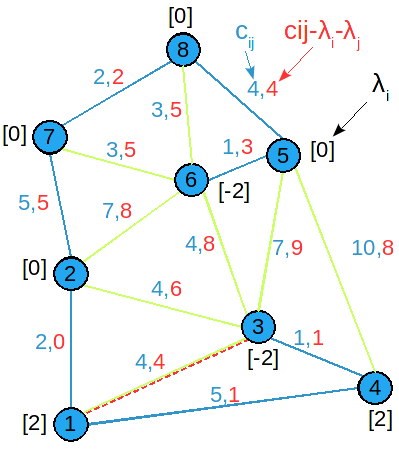
\includegraphics[height=6cm]{images/graph32.png}}
Albero di costo minimo $SST$ usando i costi $\{c_{ij},\lambda_{i}-\lambda_{j}\}$
\begin{flalign*}
	& SST={(1,2),(1,4),(3,4),(7,8),(5,6),(5,8),(2,7)} \\
	& v(SST)=16
\end{flalign*}
Nella soluzione prodotta per $\lambda^{1}=(2,0,-2,2,0,-2,0,0)$ si ha
\begin{equation*}
	d^{1}=(3,2,2,2,2,1,2,2)
\end{equation*}

\subsubsection{Nuova iterazione per $\boldsymbol{k\gets k+1}$ ossia $\boldsymbol{k=2}$}
\begin{equation*}
	\lambda_{i}^{2}=\lambda_{i}^{1}-\alpha_{2}\cdot\frac{(z^{*}-L(\lambda^{1}))}{\sum_{i}(d_{i}^{1}-2)^{2}}\cdot;\;\;\;\;i=1,\dots,n
\end{equation*}
dove $\alpha_{2}=\alpha_{1}/2=1$
\begin{equation*}
	\lambda_{i}^{2}=\lambda_{i}^{1}-1\cdot\frac{5}{2}\cdot(d_{i}^{1}-2)
\end{equation*}
Quindi
\begin{flalign*}
	& \lambda_{1}^{2}=2-\frac{5}{2}-1=-\frac{1}{2} \\
	& \lambda_{i}^{2}=\lambda_{i}^{1},\;\;\;\;i=2,3,4,5 \\
	& \lambda_{6}^{2}=-2-\frac{5}{2}\cdot(-1)=-2+\frac{5}{2}=\frac{1}{2} \\
	& \lambda_{7}^{2}=\lambda_{7}^{1},\;\lambda_{8}^{2}=\lambda_{8}^{1} \\
	& \\
	& \lambda_{2}=(-\frac{1}{2},0,-2,+2,0,\frac{1}{2},0,0)
\end{flalign*}

\subsubsection{Calcolo di $\boldsymbol{L(\lambda^{2})}$}
\centerline{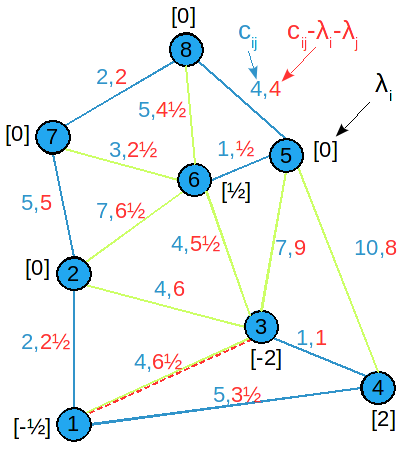
\includegraphics[height=6cm]{images/graph33.png}}
Albero a costo minimo $SST$ usando i costi $\{c_{ij}-\lambda_{i}-\lambda_{j}\}$
\begin{flalign*}
	& SST=\{(5,6),(3,4),(7,8),(1,2),(6,7),(1,4),(2,7)\} \\
	& v(SST)=17\\
\end{flalign*}
Arco a costo minimo $\notin SST$ è $(5,8)$ e $c_{l_{min}}'=4$
\begin{equation*}
	L(\lambda^{2})=v(SST)+c_{l_{min}}+2\sum_{i}\lambda_{i}=17+4+0=21
\end{equation*}
Nella soluzione per $\lambda^{2}=(-\frac{1}{2},0,-1,+2,0,\frac{1}{2},0,0)$ si ha che
\begin{equation*}
	d^{2}=(2,2,1,2,2,2,3,2)
\end{equation*}
\subsubsection{Nuova iterazione per $\boldsymbol{k=3}$, $\boldsymbol{\alpha_{3}=\frac{1}{2}\;(\alpha_{3=\alpha_{2}/2})}$}
\begin{equation*}
	\lambda_{i}^{3}=\lambda_{i}^{2}-\alpha_{3}\cdot\frac{(z^{*}-L(\lambda^{2}))}{\sum_{i}(d_{i}^{2}-2)^{2}}\cdot(d_{i}^{2}-2)
\end{equation*}
ovvero
\begin{equation*}
	\lambda_{i}^{3}=\lambda_{i}^{2}-\frac{1}{2}\cdot\frac{4}{2}\cdot(d_{i}^{2}-2)
\end{equation*}
Quindi
\begin{flalign*}
	& \lambda_{3}^{3}=-2-1\cdot(-1)=-1\\
	& \lambda_{7}^{3}=0-1\cdot 1=-1 \\
	& \textnormal{altrimenti }\lambda_{i}^{3}=\lambda_{i}^{2},\;\;\;\;\forall i\neq=3,7 \\
	& \lambda^{3}=(-\frac{1}{2},0,-1,+2,0,\frac{1}{2},-1,0)	
\end{flalign*}
\subsubsection{Calcolo di $\boldsymbol{L(\lambda^{3})}$}
\centerline{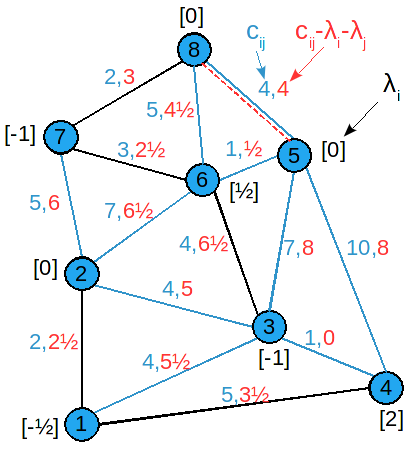
\includegraphics[height=6cm]{images/graph34.png}}
\begin{flalign*}
& SST=\{(3,4),(5,6),(1,2),(7,8),(1,4),(7,6),(3,6)\} \\
& v(SST)=17.5\\
\end{flalign*}
Arco a costo minimo $\notin SST$ è $(5,8)$ e $c_{l_{min}}'=4$
\begin{equation*}
L(\lambda^{2})=v(SST)+c_{l_{min}}+2\sum_{i}\lambda_{i}=17.5+4=21.5
\end{equation*}
\begin{equation*}
d^{3}=(2,1,2,2,2,3,2,2)
\end{equation*}
\subsubsection{Nuova iterazione per $\boldsymbol{k=4}$, $\boldsymbol{\alpha_{4}=\frac{1}{4}}$}
\begin{equation*}
	\lambda_{i}^{4}=\lambda_{i}^{3}-\frac{1}{4}\cdot\frac{3.5}{2}(d_{i}^{3}-2)
\end{equation*}
per semplificare si usi:
\begin{equation*}
	\lambda_{i}^{4}=\lambda_{i}^{3}-\frac{1}{2}\cdot(d_{i}^{3}-2)
\end{equation*}
\textit{continuare per esercizio...}

\subsection{Rilassamento 1-TREE}
\textit{Held and Karp}
\begin{itemize}
	\item Si rimuova dal grafo un vertice;
	\item Si calcolo lo shortest spanning tree (SST) sul grafo rimanente;
	\item Si aggiungano i due links di costo minimo che incidono sul vertice rimosso;
	\item Il lower bound è dato dalla somma del costo dello $SST$ e dei costi dei due link aggiunti
\end{itemize}
\centerline{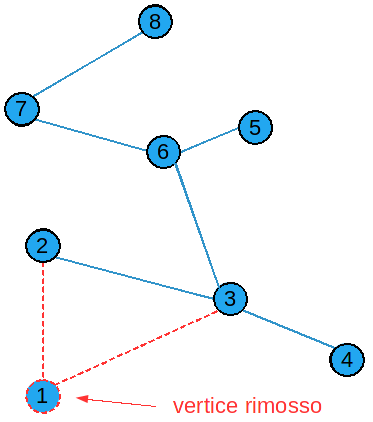
\includegraphics[height=5cm]{images/graph35.png}}
\subsection{Regola di branching TSP simmetrico}
Al nodo $K$ dell'albero decisionale: scegli un vertice $i$ il cui grado sia maggiore a $2$ è due links $a$ e $b$ che nello $SST$ incidono su $i$ e \underline{liberi}.\\
Genera $3$ nodi come segue\\
\centerline{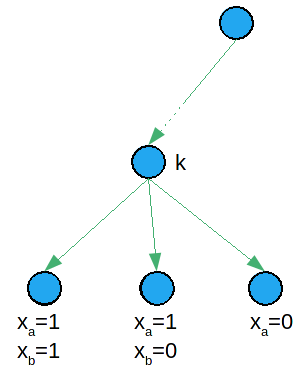
\includegraphics[height=5cm]{images/graph36.png}}
\chapter{Programmazione dinamica}
\section{Motivazioni}
Si consideri il problema del cammino minimo di un grafo da $s$ a $t$.\\
\centerline{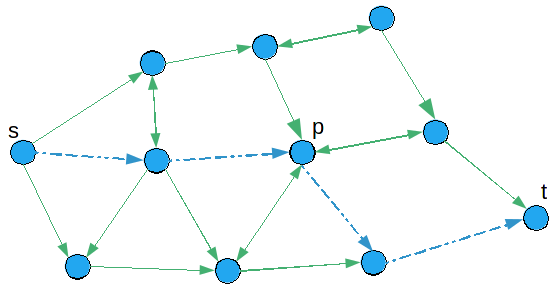
\includegraphics[height=4.25cm]{images/graph37.png}}
\subsection{Osservazione 1}
Se il cammino minimo $(s,t)$ passa per il vertice $p$, allora, i sottocammini $(s,p)$ e $(p,t)$ sono i cammini minimi di $s$ a $p$ e da $p$ a $t$, rispettivamente.
\subsubsection{Dimostrazione}
Se per assurdo uno dei due cammini $(s,p)$ e $(p,t)$ non fosse un cammino minimo, allora $(s,t)$ non potrebbe essere il cammino minimo da $s$ a $t$.
\subsection{Osservazione 2}
Indichiamo con $d(v)$ il costo del cammino minimo da $s$ a $v$ e dall'osservazione $1$ si ottiene che se conosciamo il costo di $d(i)$ del cammino minimo da $s$ ad ogni predecessore $i\in \Gamma^{-1}(v)$ del vertice $v$ allora:
\begin{equation}
	d(v)=\underset{i\in\Gamma^{1}(v)}{min}[d(i)+c_{iv}] \label{eq:4.1}
\end{equation}
Tale osservazione non è sufficiente per stabilire un algoritmo per calcolare il cammino minimo in un qualsiasi tipo di grafo.\\
È sufficiente per grafi aciclici.

\subsection{Osservazione 3}
Sia $G=(V,A)$ un grafo orientato aciclico di $n=|V|$ vertici e $m=|A|$ archi i cui vertici sono ordinati così che $i<j$ $\forall(i,j)\in A$ (ovvero $i<v$, $\forall i\in\Gamma^{-1}(v)$).\\
Supponiamo siano noti i costi $d(1),d(2),\dots,d(k)$ dei cammini minimi dal vertice $1$ ai vertici $(1,2,\dots,k)\subset V$.\\
Allora, per come è stato definito il grafo aciclico $G$, sono noti i costi $d(i)$, $\forall i\in\Gamma^{-1}_{k+1}$ e quindi
\begin{equation*}
	d_{k+1}=\underset{i\in\Gamma^{-1}_{k+1}}{min}[d(i)+c_{i,k+1}]
\end{equation*}

\section{Algoritmo}
\begin{enumerate}
	\item Poni $d(1)=0$, $d(2)=\dots=d(n)=\infty$;
	\item Per $v=2,\dots,n$ calcola $d(v)=\underset{i\in\Gamma^{-1}(v)}{min}[d(i)+c_{iv}]$.
\end{enumerate}
\centerline{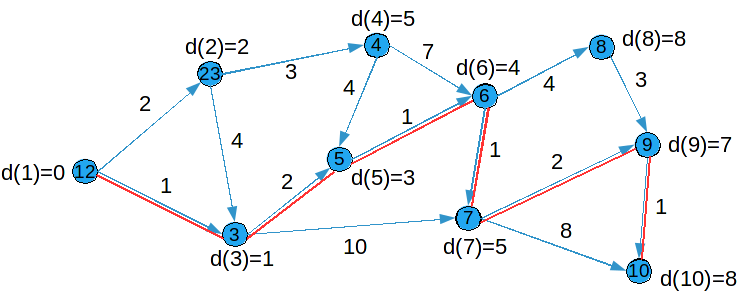
\includegraphics[height=5cm]{images/graph38.png}}

\section{Algoritmo Forward (grafi aciclici)}
\begin{enumerate}
	\item Poni $d(1)=0$ e $d(j)=\infty$, $\forall j\in V\setminus\{1\}$;
	\item sia $v=1$;
	\item per ogni $j\in\Gamma(v)$ aggiorna:
	\begin{equation*}
		d(j)=min[d(j),d(v)+c_{vj}]
	\end{equation*}
	\item Se $v=n-1$ STOP, altrimenti poni $v=v+1$ e ritorna allo step 3.
\end{enumerate}

\textbf{Caso generale}: grafi orientati con cicli e costi degli archi $c_{ij}$ non-negativi.\\
Non si può applicare direttamente la ricorsione poichè è necessario imporre un ordine con cui calcolare la \ref{eq:4.1}.

\section{Algoritmo di Bellman}
Sia $D(k,j)$ il costo del cammino minimo da $s$ a $j$ contenente al più $k$ archi.\\
Si hanno due casi:
\begin{enumerate}
	\item Il cammino minimo di costo $D(k,j)$ contiene al più $k-1$ archi, quindi
	\begin{equation*}
		D(k,j)=D(k-1,j)
	\end{equation*}
	\item Il cammino minimo di costo $D(k,j)$ contiene $k$ archi, quindi
	\begin{equation}
		D(k,j)=\underset{i\in\Gamma^{-1}(j)}{min}[D(k-1,i),+c_{ij}] \label{eq:4.2}
	\end{equation}
\end{enumerate}
Partendo dalla \ref{eq:4.2} si a che la ricorsione è:
\begin{equation}
	D(k,j)=min[D(k-1,j),\underset{i\in\Gamma^{-1}(j)}{min}[D(k-1,i)+c_{ij}]] \label{eq:4.3}
\end{equation}
La ricorsione \ref{eq:4.3} impone un ordine implicito di calcolo:\\
prima $D(1,j),\ \forall j\in V$, poi $D(2,j)$, $D(3,j)$, \dots, $D(n-1,j)$.

\subsection{Schema dell'algoritmo cammini minimi da 1 ad ogni $\boldsymbol{j\in V}$}
\begin{enumerate}
	\item Definisci
	\begin{flalign*}
		& D(1,1)=0 \\
		& D(1,j)
		\begin{cases}
			c_{1j},\ \ \forall j\in\Gamma(1) \\
			\infty,\ \ \forall j\in V\setminus\Gamma(1)
		\end{cases}
	\end{flalign*}
	\item Per $k=2,\dots,n-1$ calcola
	\begin{equation*}
	D(k,j)=min[D(k-1,j),\underset{i\in\Gamma^{-1}(j)}{min}[D(k-1,i)+c_{ij}]],\ \ \ \ \forall j\in V
	\end{equation*}
	\item Poni $d(j)=D(n-1,j),\ \ \ \ \forall j\in V$
\end{enumerate}

\section{Knapsack 0-1}
Sono dati $n$ items ed un \textit{knapsack} di capacità $b$.\\
L'item $j$ ha peso $a_{j}$ e profitto $c_{j}$.\\
Si vuole riempire il knapsack massimizzando il profitto complessivo degli items caricati.\\
Assumiamo che i coefficienti $\{a_{j}\}$ e $b$ siano interi positivi
\begin{equation*}
	KP
	\begin{cases}
		z = max\sum_{j=1}^{n}c_{j}x_{j} \\
		\ \ \ \ \ \ \ \ \ \ \ \ \sum_{j=1}^{n}a_{j}b_{j}\le b \\
		\ \ \ \ \ \ \ \ \ \ \ \ x_{j}\in\{0,1\},\ \ j=1,\dots,n
	\end{cases}
\end{equation*}

\subsection{Esempio}
\begin{displaymath}
	\begin{cases}
		z=max 10x_{1}+7x_{2}+25x_{3}+24x_{4}\\
		\ \ \ \ \ \ \ \ \ \ \ \ \ 2x_{1}+1x_{2}+6x_{3}+5x_{4}\le 7 \\
		\ \ \ \ \ \ \ \ \ \ \ \ \ \ \,x_{j}\in\{0,1\},\ \ j=1,\dots,4
	\end{cases}
\end{displaymath}
La soluzione ottima è $x_{i}^{*}=1,\ x_{2}^{*}=0,x_{3}^{*}=0,x_{4}^{*}=1$.

\subsection{Osservazione 1}\label{ss:osservazione_1}
Se $x^{*}=(x_{1}^{*},x_{2}^{*},\dots,x_{n}^{*})$ è una soluzione ottima di $KP$ allora $(x_{1}^{*},x_{2}^{*},\dots,x_{k}^{*})$ con $k\le n$ è una soluzione ottima del seguente sottoproblema $KP_{k}(q)$.
\begin{equation*}
	KP_{k}(q)
	\begin{cases}
		f_{k}(q)=max\sum_{j=1}^{k}c_{j}x_{j}\\
		\ \ \ \ \ \ \ \ \ \ \ \ \ \ \ \ \ \sum_{j=1}^{k}a_{j}x_{j}\le q \\
		\ \ \ \ \ \ \ \ \ \ \ \ \ \ \ \ \ x_{j}\in\{0,1\},\ \ j=1,\dots,k \\
		\ \ \ \ \ \ \ \ \ \ \textnormal{ dove }q=\sum_{j=1}^{k}a_{j}x_{j}^{*}
	\end{cases}
\end{equation*}
\clearpage
\subsubsection{Esempio}
$(x_{1}^{*}=1,x_{2}^{*}=0,x_{3}^{*}=0)$ deve essere la soluzione ottima del seguente problema
\begin{equation*}
	KP_{3}(q)
	\begin{cases}
		f_{3}(q)=max 10x_{1}+7x_{2}+25x_{3} \\
		2x_{1}+1x_{2}+6x_{3}\le q=2 \\
		x_{1},x_{2},x_{3}\in\{0,1\}
		\textnormal{dove }q=2x_{1}^{*}+1x_{2}^{*}+6x_{3}^{*}=2
	\end{cases}
\end{equation*}
La dimostrazione dell'\hyperref[ss:osservazione_1]{osservazione 1} è ovvia!\\
Si consideri la famiglia degli $n(b+1)$ sottoproblemi
\begin{equation*}
	\{KP_{k}(q):1\le k\le n,\ 0\le q\le b\}\ \ \ \ q\textnormal{ intero}
\end{equation*}
dove $q$ è detto 'stato' e $k$ è detto 'stadio'.\\
Il problema originario $KP$ è un membro di tale famiglia: $KP=KP_{n}(b)$ e $z=f_{n}(b)$ ($z$: costo ottimo di $KP$).\\

Come risolvere $KP_{k}(q)$ per un dato $k\le n$ e $q\le b$?

Sia $(x_{1}^{*},\dots,x_{k-1}^{*},x_{k}^{k})$ la soluzione ottima di $KP_{k}(q)$ di costo $f_{k}(q)$. Si hanno due casi:
\begin{enumerate}
	\item $x_{k}^{*}=0$, allora $q=\sum_{j=1}^{k}a_{j}x_{j}^{*}\equiv\sum_{j=1}^{k-1}a_{j}x_{j}^{*}$ e quindi $((x_{1}^{*},\dots,x_{k-1}^{*})$ è la soluzione ottima di $KP_{k-1}(q)$ ovvero $f_{k}(q)=f_{k-1}(q)$;
	\item $x_{k}^{*}=1$, allora $q=\sum_{j=1}^{k-1}a_{j}x_{j}^{*}+a_{k}$ e quindi $(x_{1}^{*},\dots,x_{k-1}^{*})$ è la soluzione ottima di $KP_{k-1}(q-ax)$ ovvero $f_{k}(q)=f_{k-1}(q-ax)+c_{k}$
\end{enumerate}
Se conosciamo $f_{k-1}(q)$ e $f_{k-1}(q-ax)$ si ha la seguente ricorsione:
\begin{equation*}
	f_{k}(q)=max[f_{k-1}(q),\ f_{k-1}(q-ax)+c_{k}]
\end{equation*}
Per calcolare $f_{k}(q)$, $\forall q$ per un dato $k$ dobbiamo conoscere i valori $f_{k-1}(q)$, $\forall q$.\\
Partiamo ponendo $f_{0}(q)=0$, per ogni $q$ tale che $0\le q\le b$. Ciò consente di calcolare $f_{1}(q)$, $\forall q$, mediante la ricorsione.\\
Quindi, $f_{1}(\cdot)$ consente di calcolare $f_{2}(\cdot),\dots$, infine, $f_{n-1}(\cdot)$ consente di calcolare $f_{n}(\cdot)$.
\subsubsection{Esempio}
\begin{equation*}
	\begin{cases}
	z=max\ 10x_{1}+7x_{2}+25x_{3}+24x_{4}\\
	\ \ \ \ \ \ \ \ \ \ \ \ \ \ 2x_{1}+1x_{2}+6x_{3}+5x_{4}\le 7 \\
	\ \ \ \ \ \ \ \ \ \ \ \ \ \ x_{j}\in\{0,1\},\ \ j=1,\dots,4
	\end{cases}
\end{equation*}
\begin{equation*}
	f_{k}(q)=max[f_{k-1}(q),f_{k-1}(q-a_{k})+c_{k}],\ \ \ \ \ \forall q\le b,\ \ k=b,\dots,n
\end{equation*}
\begin{table}[!h]
	\centering
	\begin{tabular}{l|llll}
		& $f_{1}$ & $f_{2}$ & $f_{3}$ & $f_{4}$ \\ \cline{1-5}
		$q=0$ & 0 & 0 & 0 & 0 \\
		$q=1$ & 0 & 7 & 7 & 7 \\
		$q=2$ & 10 & 10 & 10 & 10 \\
		$q=3$ & 10 & 17 & 17 & 17 \\
		$q=4$ & 10 & 17 & 17 & 17 \\
		$q=5$ & 10 & 17 & 17 & 24 \\
		$q=6$ & 10 & 17 & 25 & 31 \\
		$q=7$ & 10 & 17 & 32 & 34 \\
	\end{tabular}
\end{table}

Soluzione ottima:
\begin{flalign*}
	& f_{4}(7)>f_{3}(7)\implies x_{4}^{*}=1 \\
	& f_{3}(7-5)=f_{2}(2)\implies x_{3}^{*}=0 \\
	& f_{2}(2)=f_{1}(2)\implies x_{2}^{*}=0 \\
	& f_{1}(2)>f_{0}(2)\implies x_{1}^{*}=1 \\
\end{flalign*}

\subsection{Grafo dello spazio degli stati}
Alla ricorsione
\begin{equation*}
	f_{k}(q)=max[f_{k-1}(q),f_{k-1}(q-a_{k})+c_{k}],\ \ \ \ q\le b,\ \ k=1,\dots,n
\end{equation*}
si può associare un grafo aciclico $H=(X,A)$ così fatto:
\begin{itemize}
	\item $X$ si compone di $n+1$ partizioni $X_{0},X_{1},X_{2},\dots,X_{n}$.\\
	$X_{0}=(0)$ e ogni altra partizione $X_{k}$, $k=1,\dots,n$ contiene $b+1$ vertici corrispondenti agli stati $(0,1,2,\dots,b)$;
	\item Su ogni vertice $q\in X_{k}$ terminano al più due archi: l'arco avente vertice iniziale in $q-a_{k}\in X_{k-1}$ di costo $c_{k}$ (l'arco non esiste se $q\in X_{k-1}$ o se $q-a_{k}<0$)
\end{itemize}
\centerline{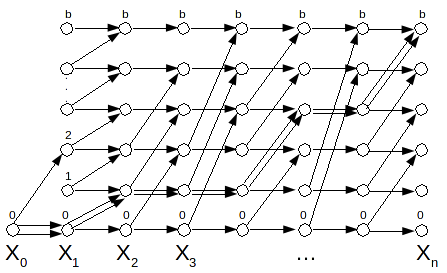
\includegraphics[height=5cm]{images/graph39.png}}
Il cammino di profitto massimo da $0\in X_{0}$ a $b\in X_{n}$ corrisponde a $f_{n}(b)$.
\subsection{Esempio}
\begin{equation*}
	\begin{cases}
		z=max\ 10x_{1}+7x_{2}+25x_{3}+24x_{4} \\
		\ \ \ \ \ \ \ \ \ \ \ \ \ \ 2x_{1}+1x_{2}+6x_{3}+5x_{4}\le 7 \\
		\ \ \ \ \ \ \ \ \ \ \ \ \ \ x_{j}\in\{0,1\},\ \ j=1,\dots,4
	\end{cases}
\end{equation*}
\centerline{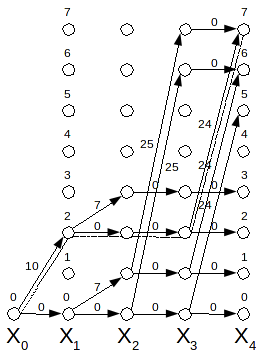
\includegraphics[height=8cm]{images/graph40.png}}
Non sono stati disegnati gli archi inutili, ovvero, non attraversabili da alcun cammino che parte da $0\in X_{0}$.\\
Il grafo mostra che è inutile calcolare $f_{1}(q)$, $q\in\{1,3,4,5,6,7\}$ ma anche $f_{2}(q)$, $q=4,\dots,7$, etc.\\\\
Qual è un algoritmo migliore per implementare la ricorsione per il knapsack 0-1?

\subsection{Ricorsione Froward - Knapsack 0-1}
\begin{enumerate}
	\item Poni $f_{0}(0)=0$ e $f_{0}(q)=-\infty$, $q=1,\dots,b$. Sia $k=0$;
	\item inizializza $f_{k+1}(q)=-\infty$, $q=0,1,\dots,b$;
	\item Per ogni $q=0,1,\dots,b$ tale che $f_{k}(q)\ge 0$ aggiorna 
	\begin{equation*}
		f_{k+1}(q)=max\ [f_{k+1}(q),f_{k}(q)] 
	\end{equation*}
	se $q+a_{k+1}\le b$ allora
	\begin{equation*}
		f_{k+1}(q+a_{k+1})=max\ [f_{k+1}(q+a_{k+1}),f_{k}(q)+c_{k+1}]
	\end{equation*}
	\item Se $k=n-1$ \textit{STOP}, altrimenti poni $k=k+1$ e ritorna allo step 2.
\end{enumerate}

\section{Programmazione a numeri interi}
\begin{flalign*}
	& F^{*}=Min\;\,\sum_{j=1}^{n}C_{j}x_{j} \\
	& \ \ \ \ \ \ \ \ \ \ \ \ \ \ \ \sum_{j=1}^{n}a_{1j}x_{j}=b_{1} \\
	& \ \ \ \ \ \ \ \ \ \ \ \ \ \ \ \sum_{j=1}^{n}a_{2j}x_{j}=b_{2} \\
	& \ \ \ \ \ \ \ \ \ \ \ \ \ \ \ \ \ \ \vdots\ \ \ \ \ \ \ \vdots \\
	& \ \ \ \ \ \ \ \ \ \ \ \ \ \ \ \sum_{j=1}^{n}a_{mj}x_{j}=b_{m} \\
	& \ \ \ \ \ \ \ \ \ \ \ \ \ \ \ x_{j}\ge 0 \textnormal{ e intero}
\end{flalign*}
Per semplicità assumiamo che
\begin{flalign*}
	& a_{ij}\ge 0\ \ \ \ \ \ \ \forall i,j \\
	& \ \,b_{i}\ge 0\ \ \ \ \ \ \;\forall i
\end{flalign*}

\section{Programmazione Dinamica}
\begin{flalign*}
	& F_{k}(\ubar{v})=Min\ \sum_{j=1}^{k}C_{j}x_{j} \\
	& \ \ \ \ \ \ \ \ \ \ \ \ \ \ \ \ \ \ \sum_{j=1}^{k}a_{1j}x_{j}=v_{1} \\
	& \ \ \ \ \ \ \ \ \ \ \ \ \ \ \ \ \ \ \sum_{j=1}^{k}a_{2j}x_{j}=v_{2} \\
	& \ \ \ \ \ \ \ \ \ \ \ \ \ \ \ \ \ \ \ \ \vdots\ \ \ \ \ \ \ \vdots \\
	& \ \ \ \ \ \ \ \ \ \ \ \ \ \ \ \ \ \ \sum_{j=1}^{k}a_{mj}x_{j}=v_{m} \\
	& \ \ \ \ \ \ \ \ \ \ \ \ \ \ \ \ \ \ x_{1},x_{2},\dots,x_{k}\ge 0 \textnormal{ e intero}
\end{flalign*}
$F_{k}(V)$ venga calcolato per $k=1,\dots,n$; $\forall \ubar{v}\le \ubar{b}$ e $\ubar{v}\ge 0$.\\
La soluzione ottima è data da
\begin{equation*}
	F^{*}=F_{n}(\ubar{b})
\end{equation*}

\section{Ricorsione di Programmazione Dinamica}
Le funzioni $F_{k}(\ubar{v})$ si possono calcolare come segue:
\begin{equation*}
	F(\ubar{v})=Min\ \{F_{k-1}(\ubar{v}),\ \underset{\underset{x_{k}\ intero}{x_{k}>0}}{Min}[F_{k-1}(\ubar{v}-a^{k}x_{k})+c_{k}x_{k}]\})
\end{equation*}
per $k=1,\dots,n$; $\forall \ubar{v}\le \ubar{b}$.\\
La ricorsione richiede di conoscere $F_{0}(\ubar{v})$
\begin{equation*}
	F_{0}(\ubar{v})
	\begin{cases}
		0 \textnormal{ per }v={0}\\
		\infty \textnormal{ per ogni } 0 < \ubar{v}\le b
	\end{cases}
\end{equation*}
$k$ rappresenta lo \textbf{stadio} della ricorsione mentre $v$ è la \textbf{variabile di stato}.

\section{Programmazione Dinamica: il TSP}
È dato un grafo $G=(X,A)$ di $n=|X|$ vertici ed $m=|A|$ archi. Ad ogni arco $(x_{i},x_{j})\in A$ è associato un costo $c_{ij}$.

Determinare il cammino di costo minimo che parte da $x_{1}$, attraversa tutti i vertici di $G$ una ed una sola volta e termina in $x_{1}$.
\begin{itemize}
	\item[] $f(S,x_{i})$: costo minimo di un cammino che parte da $x_{i}$, attraversa tutti i vertici di $S\in X\setminus{x_{i}}$ una ed una sola volta e termina in $x_{i}\in S$.
\end{itemize}

\subsection{Ricorsione per il calcolo di $\boldsymbol{f(S,x_{i})}$}
\begin{equation*}
	f(S,x_{i})=\underset{x_{j}\in S\setminus{x_{i}}}{Min}\{f(S\setminus{x_{i}},x_{j})+c_{ji}\}
\end{equation*}
Le $f(S,x_{i})$ vanno calcolate:
\begin{equation*}
	\forall S\subseteq X \textnormal{ tale che }x_{1}\in S,\ |S|\ge 2,\ \forall x_{i}\in S\setminus{x_{1}}
\end{equation*}
\subsubsection{Calcolo del valore $\boldsymbol{z^{*}}$ della soluzione ottima}
\begin{equation*}
	z^{*}=\underset{x_{i}\in X\setminus\{x_{1}\}}{Min}\{f(X,x_{i})+c_{i1}\}
\end{equation*}
È richiesta la seguente inizializzazione:
\begin{equation*}
	f(\{x_{1}\},x_{1})=0
\end{equation*}
\clearpage
\subsection{Considerazioni computazionali}
Il calcolo di $f(S,x_{i})$ richiede di conoscere il valore di $f(S\setminus\{x_{i}\}, x_{j})$ $\forall x_{j}\in S\setminus\{x_{i}\}$\\\\
\textbf{Esempio:} calcolo di $f(\{x_{2},x_{3},x_{4}x_{5}\},x_{2})$
\begin{equation*}
	f(\{x_{2},x_{3},x_{4}x_{5}\},x_{2})=\underset{x_{j}\in\{x_{3},x_{4},x_{5}\}}{Min}[f(\{x_{3},x_{4},x_{5}\},x_{j})+c_{j2}]
\end{equation*}
e quindi bisogna conoscere:
\begin{equation*}
	f(\{x_{3},x_{4}x_{5}\},x_{3});\ \ f(\{x_{3},x_{4}x_{5}\},x_{4});\ \ f(\{x_{3},x_{4}x_{5}\},x_{5})
\end{equation*}

Le \textbf{variabili di stato} sono rappresentate da
\begin{equation*}
	(S,x_{i});\ \ \ \ \forall\ S\subseteq X\setminus\{x_{i}\},\ \ \forall\ x_{i}\in S
\end{equation*}
Lo stadio può essere definito in modi diversi; deve corrispondere al sequente principio:\\

"se lo stato $(S,x_{i})$ è associato allo stadio $K$ allora ognuno degli stati $(S\setminus\{x_{i}\},x_{j})$ deve essere associato ad uno stadio $K^{'}<K^{''}$."\\

\textbf{Ad esempio:} stadio: $|S|$ cardinalità di S.\\
È ovvio che allo stadio 1 vengono calcolate le $f(S,x_{i})$ $\forall\ S$ per cui $|S|=1$.\\
Allo stadio 2 si calcola $f(S,x_{i})$, $\forall\ S$ per cui $|S|=2$.\\
\vdots\\
Allo stadio k si calcola $f(S,x_{i})$, $\forall\ S$ per cui $|S|=k$ e quindi sono note le $f(S\setminus\{x_{i}\},x_{j})$ in quanto sono state calcolate allo stadio $k-1$.\\

Lo stadio può essere definito diversamente:
\begin{itemize}
	\item Si associ un peso $q_{i}\ge 1$ ad ogni $x_{i}\in X$. Si assegni ad ogni stato $(S,x_{i})$ allo stadio $\sum_{i\in S}^{q_{i}}$. In tal modo gli stati vengono suddivisi in $\sum_{i=1}^{n}q_{i}$ stadi;
	\item si noti che questa definizione è corretta, infatti dato lo stato $(S,x_{i})$ corrispondente a $\sum_{i\in S}q_{i}=q(S)$ ogni stato $(S\setminus\{x_{i},x_{j}\})$ corrisponde allo stadio $q(S)-q_{i}$.
\end{itemize}
È banale notare che ponendo $q_{i}=1$, $\forall\ x_{i}\in X$ lo stadio corrisponde alla cardinalità di $S$ (come visto in precedenza).

\subsection{Esempio del TSP con 5 città}
$[c_{ij}]=
	\begin{bmatrix}
		- & 6 & 11 & 3 & 4 \\
		7 & - & 14 & 8 & 10 \\
		12 & 5 & - & 10 & 2 \\
		6 & 15 & 7 & - & 5 \\
		4 & 9 & 8 & 13 & 6 -
	\end{bmatrix}$\\
	
Applichiamo la ricorsione:
\begin{equation*}
	f(S,x_{i})=\underset{x_{j}\in S\setminus\{x_{i}\}}{Min}\{f(S\setminus\{x_{i}\},x_{j})+c_{ji}\}
\end{equation*}
Inizializzazione:
\begin{equation*}
	f(\{x_{i}\},x_{i})=c_{1i};\ \ \ \ \forall\ x_{i}\in X\setminus\{x_{1}\}
\end{equation*}
\begin{flalign*}
	& f(\{2\},2)=6\\
	& f(\{3\},3)=11\\
	& f(\{4\},4)=3\\
	& f(\{5\},5)=4\\
\end{flalign*}

\subsubsection{Stadio 2: Calcolo $\boldsymbol{f(S,x_{i}),\ \forall\ S\subset X\setminus\{x_{i},\ s.t.\ |S|=2;\ \forall\ x_{i}\in S\}}$}
\begin{flalign*}
	& f(S,x_{i})=\underset{x_{j}\in S\setminus\{x_{j}\}}{Min}\{f(S\setminus\{x_{i}\},x_{j})+c_{ji}\} \\\\
	& f(\{2,3\},2)=f(\{3\},3)+c_{3,2}=11+5=16 \\
	& f(\{2,3\},3)=f(\{2\},2)+c_{2,3}=6+14=20 \\\\
	& f(\{2,4\},2)=f(\{4\},4)+c_{4,2}=3+15=18 \\
	& f(\{2,4\},4)=f(\{2\},2)+c_{2,4}=6+8=14 \\\\
	& f(\{2,5\},2)=f(\{5\},5)+c_{5,2}=4+9=13 \\
	& f(\{2,5\},5)=f(\{2\},2)+c_{2,5}=6+10=16 \\
\end{flalign*}
\clearpage
Similarmente:
\begin{flalign*}
	& f(\{3,4\},3)=10 \\
	& f(\{3,4\},4)=21 \\\\
	& f(\{3,5\},3)=12 \\
	& f(\{3,5\},5)=13 \\\\
	& f(\{4,5\},4)=17 \\
	& f(\{4,5\},5)=8 \\\\
\end{flalign*}
\subsubsection{Stadio 3: $\boldsymbol{f(S,x_{i}),\ \forall\ S\subset X\setminus\{x_{i},\ s.t.\ |S|=3;\ \forall\ x_{i}\in S\}}$}
\begin{flalign*}
	& f(\{2,3,4\},2)=\underset{x_{j}\in\{3,4\}}{Min}\{f(\{3,4\},x_{j})+c_{j2}\}\\\\
	& f(\{2,3,4\},2)=Min\ \{f(\{3,4\},3)+c_{3,2};\ f(\{3,4\},4)+c_{4,2}\}=Min\ \{10+5;\ 21+15\}=15 \\
	& f(\{2,3,4\},3)=Min\ \{f(\{2,4\},2)+c_{2,3};\ f(\{2,4\},4)+c_{4,3}\}=Min\ \{18+4;\ 14+7\}=21 \\
\end{flalign*}
Similarmente:
\begin{flalign*}
	& f(\{2,3,4\},4)=24 \\\\
	& f(\{2,3,5\},2) = 17;\ \ \ \ \ f(\{2,3,5\},3)=24;\ \ \ \ \ f(\{2,3,5\},5)=22 \\
	& f(\{2,4,5\},2) = 17;\ \ \ \ \ f(\{2,4,5\},4)=21;\ \ \ \ \ f(\{2,4,5\},5)=19 \\
	& f(\{3,4,5\},3) = 16;\ \ \ \ \ f(\{3,4,5\},4)=22;\ \ \ \ \ f(\{3,4,5\},5)=12 \\
\end{flalign*}
\subsubsection{Stadio 4}
\begin{equation*}
	f(\{2,3,4,5\},2)=\underset{x_{j}\in\{3,4,5\}}{Min}\{f(\{3,4,5\},x_{j})+c_{j2}\}
\end{equation*}
da cui
\begin{flalign*}
	& f(\{2,3,4,5\},2)=Min\ \{f(\{3,4,5\},3)+c_{3,2},\ f(\{3,4,5\},4)+c_{4,2},\ f(\{3,4,5\},5)+c_{5,2}\} = \\
	& \qquad\qquad\qquad\qquad Min\{16+5;\ 22+15;\ 12+9\}=21
\end{flalign*}
\clearpage
Similarmente
\begin{flalign*}
	& f(\{2,3,4,5\},3)=27 \\
	& f(\{2,3,4,5\},4)=25 \\
	& f(\{2,3,4,5\},5)=23 \\
\end{flalign*}
\subsubsection{Soluzione ottima}
\begin{flalign*}
	& z^{*}=\underset{x_{j}\in\{2,3,4,5\}}{Min}\{f(\{2,3,4,5\},x_{i})+c_{i1}\}= \\
	& \ \ \ =\{21+7;\ 27+12;\ 25+6;\ 23+4\}=27
\end{flalign*}

\newpage
\subsubsection{Spazio degli stati del TSP}
\begin{figure}[h]
	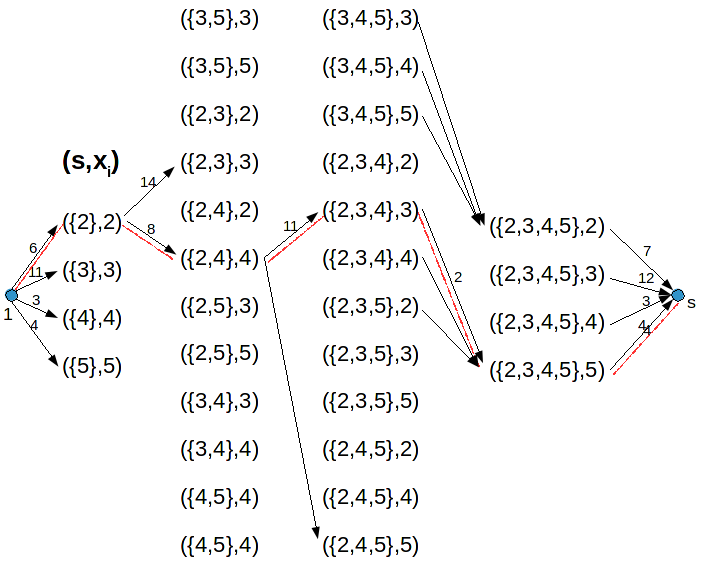
\includegraphics[height=14cm]{images/graph41.png}
	\caption{Solo alcuni degli archi sono raffigurati}
\end{figure}

\section{Ricorsione Forward per il TSP}
\begin{enumerate}
	\item $\mathscr{L}_{0}=\{(\{1\},1)\}$, $f(\{1\},1)=0$, $p(\{1\},1)=0$. Inizializza $\mathscr{L}_{r}=\emptyset$, $r=1,\dots,n$. Definisci $k=1$.
	\item Espansione degli stati del set $\mathscr{L}_{k-1}$: per ogni stato $(S,i)\in\mathscr{L}_{k-1}$ ripeti lo step 3.
	\item Genera/Aggiorna gli stati di $\mathscr{L}_{k}$ raggiungibili da $(S,i)$: per ogni vertice $j\in\Gamma_{i}\setminus S$ considera lo stato $(S',i)$, dove $S'=S\cup\{j\}$, che si ottiene aggiungendo l'arco $(i,j)$.\\
	Il costo di $(S',j)$ è $h=f(S,i)+c_{ij}$.\\
	Si hanno i seguenti casi:
	\begin{itemize}
		\item $(S',j)\in\mathscr{L}_{k}$, allora $\mathscr{L}_{k}=\mathscr{L}_{k}\cup \{f(S',j)\}$ e $f(S',j)=h$. Poni $p(S',j)=(S,i)$;
		\item $(S',j)\in\mathscr{L}_{k}$ ma $f(S',j)>h$, allora $f(S',j)=h$ e $p(S',j)=(S,i)$.
	\end{itemize}
	\item Poni $k=k+1$; se $k\le n$ vai allora step 2.
	\item Il costo ottimo $z^{*}$ del TSP si ottiene come segue:
	\begin{equation*}
		z^{*}=\underset{(X,j)\in\mathscr{L}_{n}}{Min}[f(X,j)+c_{j1}]
	\end{equation*}
\end{enumerate}

\section{Taglio 2-dimensionale a ghigliottina}
\centerline{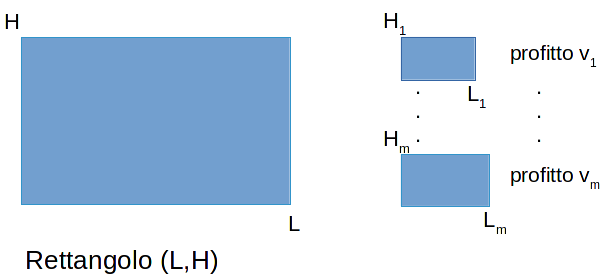
\includegraphics[height=6cm]{images/shape1.png}}
\begin{itemize}
	\item Il rettangolo e i pezzi hanno dimensioni intere e non possono essere ruotati;
	\item Sono ammessi solo tagli a ghigliottina;
	\item Ogni tipo di pezzo è disponibile in quantità illimitata
\end{itemize}

\textbf{Obiettivo}: massimizzare il profitto totale dei pezzi tagliati.

\begin{figure}[h]
	\centering
	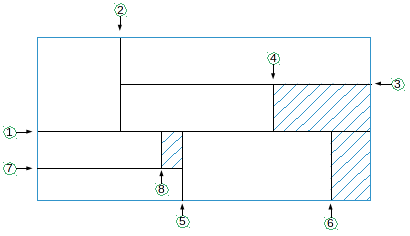
\includegraphics[height=5cm]{images/shape2.png}
	\caption{Esempio di taglio a ghigliottina}
\end{figure}
Indichiamo con:\\

$F(x,y)$ il profitto massimo per tagliare un rettangolo di dimensione $(x,y)$ con $x\le L$ e $y\le H$.\\
$F(L,H)$ il valore della soluzione ottima.

\clearpage
\subsection{Calcolo di $\boldsymbol{F(x,y)}$}
Si hanno tre casi:
\begin{enumerate}
	\item Il rettangolo $(x,y)$ contiene al più un pezzo (o nessuno) $F(x,y)=max\ [0,\ v_{i}:\ l_{i}\le x,\ h_{i}\le y,\ i=1,\dots,m]$
	\item Il rettangolo $(x,y)$ contiene due o più pezzi che per essere tagliati richiedono almeno un taglio a ghigliottina o parallelo alla lunghezza in posizione $\beta$ o parallelo all'altezza in posizione $\alpha$.
	\centerline{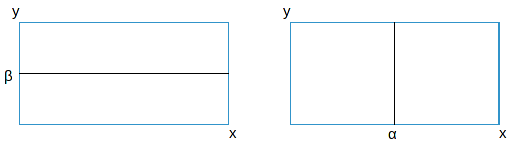
\includegraphics[height=4cm]{images/shape3.png}}
	$F(x,y)=F(x,\beta)+F(x,y-\beta)$ o $F(x,y)=F(\alpha,y)+F(x-\alpha,y)$
\end{enumerate}

\subsection{Inizializzazione}
Per ogni $x=1,...,L$ e $y=1,\dots,H$ poni
\begin{equation*}
	F^{0}(x,y)=max\ [0,\ v_{i}:\ l_{i}\le x,\ h_{i}\le y,\ i=1,\dots,m]
\end{equation*}
\begin{itemize}
	\item se $F^{0}(x,y)=v_{i^{*}}$ poni $X-cut(x,y)=l_{i^{*}}$ e $Y-cut(x,y)=h_{i^{*}}$
	\item se $F^{0}(x,y)=0$ poni $X-cut(x,y)=Y-cut(x,y)=0$
\end{itemize}
La ricorsione: per ogni $x=1,\dots,L$ e $y=1,\dots,H$ calcola
\begin{equation*}
	F(x,y)=max\ [F^{0}(x,y);\ F(x,\beta)+F(x,y-\beta),\ \beta=1,\dots,y-1,\ F(\alpha,y)+F(x-\alpha,y),\ \alpha=1,\dots,x-1]
\end{equation*}
\begin{itemize}
	\item se $F(x,y)=F(x,\beta^{*})+F(x,y-\beta^{*})$ per qualche $\beta^{*}$ poni\\ $X-cut(x,y)=0$ e $Y-cut(x,y)=\beta^{*}$
	\item se $F(x,y)=F(\alpha^{*},x)+F(x-\alpha^{*},y)$ per qualche $\alpha^{*}$ poni \\$X-cut(x,y)=\alpha^{*}$ e $Y-cut(x,y)=0$
\end{itemize}
Si può migliorare la ricorsione sostituendo
\begin{flalign*}
	& \beta=1,\dots,y-1\textnormal{ con }1\le\beta\le y/2 \\
	& \alpha=1,\dots,x-1\textnormal{ con }1\le\alpha\le x/2
\end{flalign*}
\subsection{Esempio}
Sia $y=5$
\begin{flalign*}
	F(x,5)=max\ [F^{0}(x,5),\ \overbrace{F(x,1)+F(x,4)}^{T_{1}},\overbrace{F(x,2)+F(x,3)}^{T_{2}},\underbrace{F(x,3)+F(x,2)}_{T_{3}},\underbrace{F(x,4)+F(x,1)}_{T_{4}},\dots]
\end{flalign*}
Si noti che $T_{1}\equiv T_{4}$ e $T_{2}\equiv T_{3}$ è ciò giustifica la sostituzione di $\beta=1,\dots,y-1$ con $1\le\beta\le y/2$.

Complessità: $O(L\cdot H(L+H))$.

\subsection{Normal Cuts}
Riduce la complessità in molte situazioni reali.
\begin{figure}[h]
	\centering
	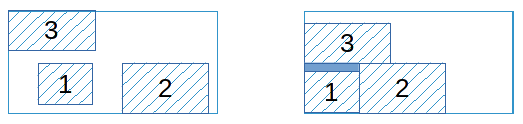
\includegraphics[height=2.0cm]{images/shape4.png}
	\caption{Sono equivalenti}
\end{figure}

I pezzi possono essere spostati in basso e a sinistra fino a che il lato sinistro e il lato inferiore di ogni pezzo sono adiacenti ad un taglio o al lato sinistro e inferiore del rettangolo.\\
I tagli a ghigliottina possono avvenire solo nelle seguenti posizioni.

\textbf{Posizioni possibili per tagli paralleli all'altezza}
\begin{equation}
	L_{0}=(x:\ x=\sum_{i=1}^{m}l_{i}\xi_{i},\ 1\le x\le L,\ \xi\ge 0\ intero)\ \ \ U(L)
\end{equation}
\textbf{Posizioni possibili per tagli paralleli alla lunghezza}
\begin{equation}
		H_{0}=(y:\ y=\sum_{i=1}^{m}h_{i}\xi_{i},\ 1\le y\le H,\ \xi\ge 0\ intero)\ \ \ U(H)
\end{equation}
Definiamo
\begin{flalign*}
	& p(x)=max\ [0,\ \alpha:\alpha\le x,\ \alpha\in L_{0}],\ \ x=1,\dots,L-1 \\
	& q(y)=max\ [0,\ \beta:\beta\le y,\ \beta\in H_{0}],\ \ y=1,\dots,H-1
\end{flalign*}
La ricorsione diviene, per ogni $x=1,\dots,L$ e $y=1,\dots,H$:
\begin{flalign*}
	& F(x,y)=max\ [F^{0}(x,y);\ F(x,\beta)+F(x,q(y-\beta)),\ \beta\in H_{0},\ \beta\le y/2,\\ 
	&\qquad\qquad\qquad\ \ \  F(\alpha,y)+F(p(x-a),y),\ \alpha\in L_{0},\ \alpha\le x/2]
\end{flalign*}

\section{Rilassamento dello spazio degli stati}
In molti casi lo spazio degli stati su cui è definita una ricorsione di programmazione dinamica (DP) ha dimensioni proibitive (si veda il caso del TSP).

\subsection{Come ridurre lo spazio degli stati}
\begin{enumerate}
	\item Eliminare stati che non possono condurre ad alcuna soluzione ottima.\\
	Ad esempio usando un lower bound.
	\item Riducendo in modo euristico gli stati fino a che lo spazio risultante non ha dimensioni "accettabili".\\
	Ad esempio scegliendo mediante qualche regola un sottoinsieme limitato di stato ad ogni stadio. Lo spazio risultante potrebbe non contenere la soluzione ottima.
	\item Contraendo più stati in un unico stato in modo che la ricorsione di $DP$ nello spazio rilassato produca un lower bound (questo metodo è noto: \textit{state space relaxation}).
\end{enumerate}

Vedremo come il metodo state space relaxation fornisca un lower bound da usare al punto 1.

\subsection{Lower bound al cammino minimo}
Il metodo della \textbf{State Space Relaxation} si basa sulla sequente semplice idea che consente di calcolare un lower bound al costo del cammino minimo in un grafo.
\begin{figure}[!h]
	\centering
	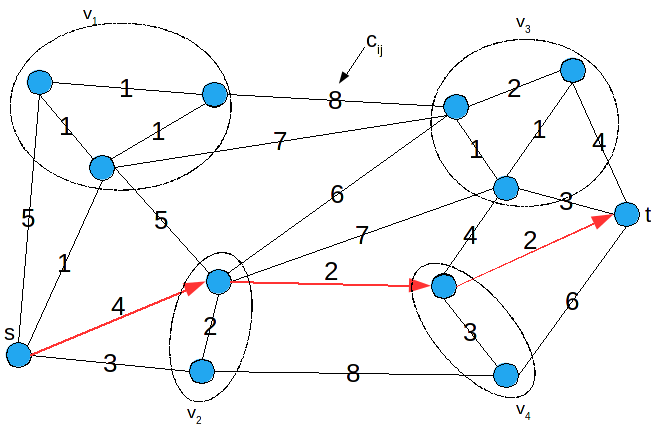
\includegraphics[height=7cm]{images/graph42.png}
	\caption{Il costo del cammino del grafo $G=(X,A)$ da $s$ a $t$ è 8}
\end{figure}

I vertici sono clusterizzati in 4 cluster come mostrato (non è importante il criterio di clustering per quanto segue).\\
Ogni $V_{k}\subset X$, $k=1,\dots,4$ e $V_{k}\cap V_{j}=\emptyset$ con $j\neq k=1,\dots,4$.

\clearpage
\textbf{Grafo rilassato $\boldsymbol{\bar{G}=(\bar{X},\bar{A}):\ \bar{X}=\{v_{0},v_{1},\dots,v_{4},v_{5}\}}$}
\begin{table}[!h]
	\begin{tabular}{m{11cm} m{5cm}}
		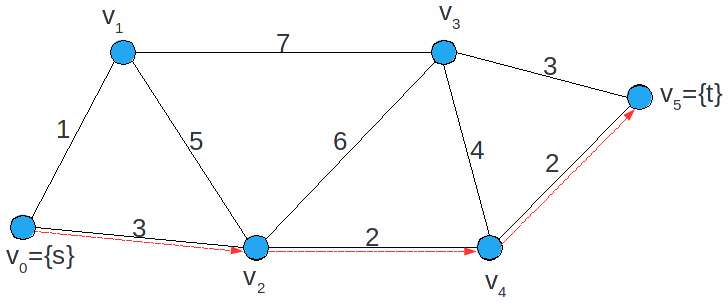
\includegraphics[height=5cm]{images/graph43.png} & \begin{equation*}
			\bar{c_{ij}}=\underset{\underset{s\in V_{j}}{r\in _V{i}}}{min}[c_{rs}]
		\end{equation*}
	\end{tabular}
\end{table}

Il costo del cammino minimo da $v_{0}$ a $v_{5}\in\bar{G}$ ($ =7$) è un valido lower bound.

\subsubsection{Esempio}
\begin{figure}[!h]
	\centering
	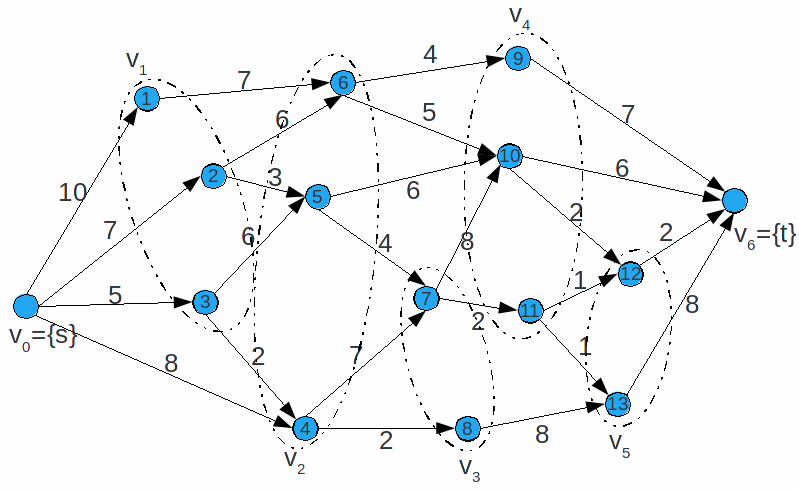
\includegraphics[height=6cm]{images/graph44.png}
\end{figure}
Nel caso di un grafo aciclico, come nell'esempio, può essere conveniente che ogni cluster $v_{k}$ sia tale che $\forall\ i,j\in v_{k}\ (i<j)$ non esista l'arco $(i,j)$ in A.

\textbf{Grafo rilassato}\\
\begin{figure}[H]
	\centering
	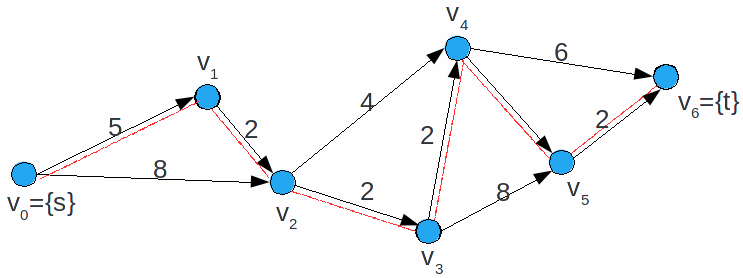
\includegraphics[height=4cm]{images/graph45.png}
\end{figure}

\subsection{Sitema discreto multistadio}
$s=(s_{1},\dots,s_{m})$: variabile di stato

$\mathscr{L}_{k}$: insieme degli stati allo stadio k

$f_{k}(s)$ è il costo minimo per cambiare lo stato del sistema dallo stato iniziale (allo stadio $0$) allo stato $s\in\mathscr{L}_{k}$ allo stadio $k$
\begin{equation*}
	f_{k}(s)=\underset{s'\in\Delta^{-1}(s)}{Min}[f_{k-1}(s')+v(s',s)],\ \ \ \ \forall\ s\in\mathscr{L}_{k}
\end{equation*}
dove $\Delta^{-1}(s)$ sono gli stati che raggiungono lo stato $s$ e $v(s',s)$ è il costo per cambiare il sistema dallo stato $s'$ allo stato $s$.

\subsubsection{Esempio: il TSP}
\begin{equation*}
	f(s,i)=\underset{j\in S\setminus\{i,1\}}{min}[f(S\setminus\{i\},j)+c_{ji}],\ \ \ \ |S|\ge 2
\end{equation*}
Definiamo (ad esempio)
\begin{flalign*}
	 & s=(S,i)                                                              \\
	 & \mathscr{L}_{k}=\{(S,i): S\subset X\ t.c.\ 1\in S,\ |S|=k,\ i\in S\} \\
	 & \Delta^{-1}(S,i)=\{(S\setminus\{i\},j):\ j\in S\{i,1\}\}             \\
	 & v((S\setminus\{i\},j),(S,i))=c_{ji}
\end{flalign*}
Sia $g(\cdot)$ una funzione di "mapping" dallo spazio degli stati $\mathscr{L}$ allo spazio ridotto $R$.\\
\centerline{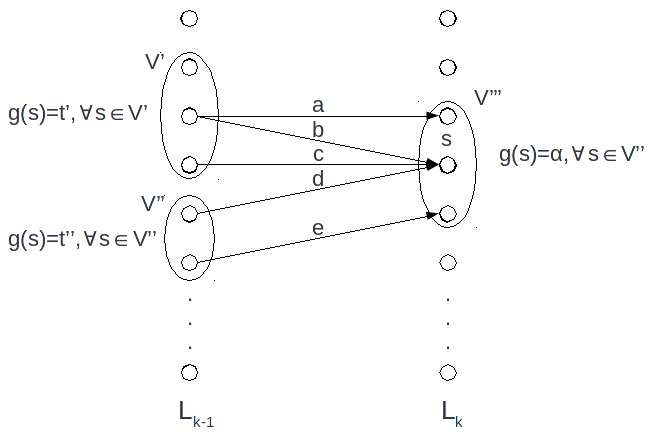
\includegraphics[height=6.1cm]{images/graph46.png}}

Più stati di $\mathscr{L}$ vengono associati ad un unico stato di $R$.

Per ogni $s'\in\Delta^{-1}(s)$ esiste l'arco $(g(s'),g(s))$.

$F^{-1}(\alpha)$: predecessori di $\alpha\in R$ (ad esempio: $F^{-1}(\alpha)=\{t',t''\}$).

$\bar{v}(\alpha,\beta)$: $min[v(s',s):\forall s',s\in\mathscr{L}\ t.c.\ g(s')=\alpha\ e\ g(s)=\beta]$.\\

\textbf{Esempio}\\

$\bar{v}(t',\alpha)=min[a,b,c]$, $\bar{v}(t'',\alpha)=min[d,e]$\\

Nello spazio $R$ la ricorsione diviene
\begin{equation*}
	f_{k}(g(s))=\underset{t\in F^{-1}(g(s))}{min}[f_{k-1}(t)+\bar{v}(t,g(s))]
\end{equation*}
Si noti che $f_{k}(g(s))\le f_{k}(s)$, $\forall\ s\in\mathscr{L}$, ovvero, $f_{k}(g(s))$ è un lower bound a $f_{k}(s)$.\\
La funzione $g(\cdot)$ deve essere tale per cui
\begin{enumerate}
	\item $p^{-1}(\alpha)$ può essere calcolato facilmente $\forall\alpha\in R$
	\item $\bar{v}(\alpha,\beta)$ può essere calcolato facilmente o approssimato con un lower bound
\end{enumerate}

\subsection{Rilassamento dello spazio degli stati per il TSP}
\begin{equation*}
	f(s,i)=\underset{j\in S\setminus{i,1}}{min}[f(S\setminus{i},j)+c_{ji}],\ \ |S|\ge 2
\end{equation*}
$(s,i)$: variabile di stato\\

Funzione di mapping: $(s,i)\rightarrow (g(s),i)$
\begin{flalign*}
	& \Delta^{-1}(s,i)=\{(S\setminus{i},j):\ j\in S\setminus\{i,1\}\} \\
	& F^{-1}(g(s),i)=\{(g(S\setminus\{i\}),j):\ j\in S\setminus\{i,1\}\}\subseteq\{g(S\setminus\{i\},j):\ j\in \Gamma^{-1}\} \\
	& v((S\setminus\{i\},j)), (s,i))=c_{ji}
\end{flalign*}
quindi $v()$ non dipende da $S$, per cui
\begin{equation*}
	\bar{v}((g(S\setminus\{i\}),j),(g(s),i))=c_{ji}
\end{equation*}
La ricorsione nello spazio rilassato diviene
\begin{equation*}
	f(g(s),i)=\underset{j\in\Gamma^{-1}\setminus\{1\}}{min}[f(g(S\setminus\{i\}),j)+c_{ji}],\ \ \ |S|\ge 2
\end{equation*}
Inizializzazione
\begin{equation*}
	f(g(\{1,i\}),i)=c_{1j},\ \ \forall\ i
\end{equation*}

\clearpage
\subsection{Funzioni di mapping $\boldsymbol{g(\cdot)}$ per il TSP}
\subsubsection{Rilassamento \textit{n-path}}
$g(S)=|S|:\ (S,i)\rightarrow(k,i)$ dove $k=|S|$
\begin{equation*}
	f(k,i)=\underset{j\in\Gamma^{-1}_{i}\setminus\{1\}}{min}[f(k-1,j)+c_{ji}],\ \ k\ge 2
\end{equation*}
Inizializza $f(1,i)=c_{1i}$, $\forall\ i$

$f(k,1)$: cammino minimo di cardinalità $k$ da 1 a $i$ (tale cammino può essere non elementare).

$z^{*}=\underset{i}{min}[f(n-1,i)+c_{i1}]$ è un lower bound al $TSP$

\begin{table}[!h]
	\begin{tabular}{m{8cm} m{5cm}}
		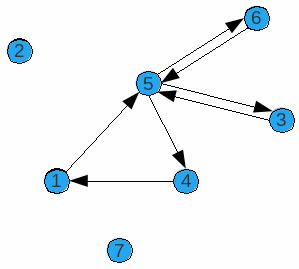
\includegraphics[height=6cm]{images/graph47.png} & Il vertice 5 è visitato 3 volte.\newline I vertici 2 e 7 non sono visitati.
	\end{tabular}
\end{table}
\textbf{Miglior lower bound}\\
Si penalizzi in modo Lagrangiano i vertici non visitati esattamente una ed una sola volta.

\clearpage
\subsection{Rilassamento q-path}
Ad ogni vertice $i$ si associ un peso $q_{i}\le 1$ e $q_{1}=0$
\begin{equation*}
	g(S)=\sum_{i\in S}q_{i}:\ (S,i)\rightarrow(q,i)\textnormal{ dove }q=\sum_{i\in S}q_{i}
\end{equation*}
\begin{equation*}
	f(q,i)=\underset{j\in\Gamma^{-1}_{i}\setminus\{1\}}{min}[f(q-q_{i},j)+c_{ji}],\ q>q_{i}
\end{equation*}
Inizializza:
\begin{flalign*}
	&f(q,i)=
	\begin{cases}
		c_{1i}, \textnormal{ se }q=q_{i} \\
		\infty, \textnormal{ altrimenti}
	\end{cases}
	,\ \ \forall i \textnormal{ e }\forall\ q=1,\dots,Q \\\\
	& \textnormal{dove }Q=\sum_{i=1}^{k}q_{i}
\end{flalign*}
Il lower bound al $TSP$ è dato da
\begin{equation*}
	z^{*}=\underset{i}{min}[f(Q,i)+c_{j1}]
\end{equation*}
Il cammino di costo $f(q,i)$ può essere non elementare e quindi anche il circuito corrispondente a $z^{*}$.\\
Un miglior lower bound, anche in questo caso, si ottiene mediante un ascent lagrangiano in cui vengono penalizzati i vertici non visitati esattamento una sola volta.

\subsection{Eliminazione dei loops di 2 vertici}
Sia $f(k,1)$ che $f(q,i)$ possono produrre cammini non elementari con loops di 2 vertici (vedi esempio)

\centerline{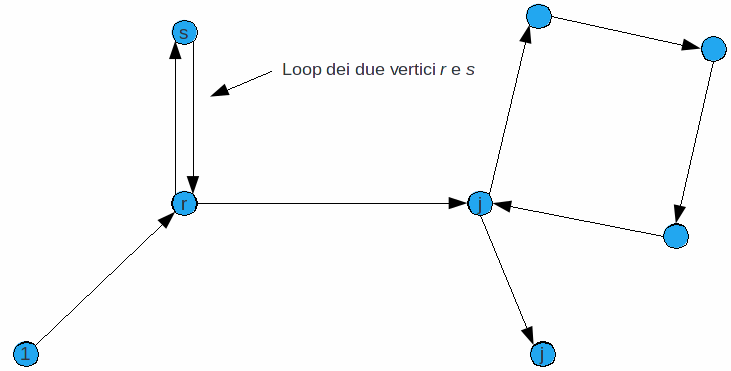
\includegraphics[height=5cm]{images/graph48.png}}
I loops di 2 vertici possono essere eliminati senza aumentare la complessità delle ricorsioni $f(k,i)$ e $f(q,i)$ con il "trucco" qui descritto per $f(q,i)$.
\clearpage
\subsubsection{Definizioni}
\begin{itemize}
	\item $f(q,i)$: costo del cammino di costo minimo e "peso" $q$ da 1 a $i$
	\item $\pi(q,i)$: vertice che precede $i$ nel cammino di costo $f(q,i)$
	\item $\phi(q,i)$: costo del cammino di costo minimo e peso $q$ da 1 a $i$ tale che il vertice che precede $i$ è diverso da $\pi(q,i)$
	\item $\gamma(q,i)$: vertice che precede $i$ nel cammino di costo $\phi(q,i)$
\end{itemize}

Per il calcolo di $f(q,i)$ e $\phi(q,i)$, $\forall\ i$ e un dato $q$ si procede come segue.

Sia $h_{ji}$ il costo del cammino minimo di peso $q$ e senza loops di 2 vertici da 1 a $i$ dove $j$ precede $i$.

$h_{ji},\ \forall i$ e $j$ si calcola come segue
\begin{equation*}
	h_{ji}=
	\begin{cases}
	f(q-q_{i},j)+c_{ji},\textnormal{ se }\pi(q-q_{i},j)\neq i \\
	\phi(q-q_{i},j)+c_{ji}\textnormal{, altrimenti}
	\end{cases},\ \forall\ i,j
\end{equation*}
Quindi calcola per ogni vertiche $i$
\begin{flalign*}
	& f(q,i)=\underset{j}{min}[h_{ji}],\textnormal{ sia $j^{*}$ il vertice che produce il $min$} \\
	& \pi(q,i)=j^{*}\\
	& \phi(q,i)=\underset{j\neq j^{*}}{min}[h_{ji}]\textnormal{, sia $\hat{j}$ il vertice che produce il $min$} \\
	& \gamma(q,i)=\hat{j}
\end{flalign*}
Inizializza
\begin{flalign*}
	& f(q,i)=
	\begin{cases}
		c_{1i}\textnormal{, se }q=q_{i} \\
		\infty\textnormal{, altrimenti}
	\end{cases} \\
	& \pi(q_{i},i)=1 \\
	& \phi(q,i)=\infty,\ \ \forall\ i \textnormal{ e }\forall\ q \\
	& \gamma(q,i)=0
\end{flalign*}

\clearpage
\subsection{Reverse function per il TSP}
$f'(S,i)$: costo del cammino che parte dalla città $i\in S$ visita una e una sola volta tutti i vertici di $S$ e termina nella città $1$.
\begin{table}[!h]
	\begin{tabular}{m{11cm} m{5cm}}
		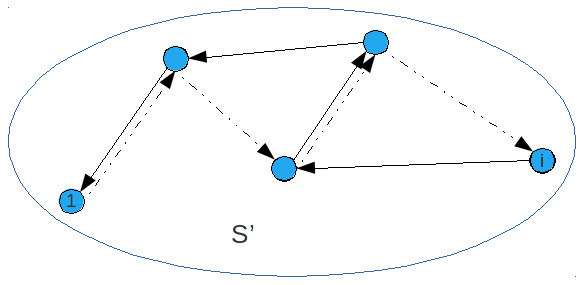
\includegraphics[height=5cm]{images/graph49.png} & 
		Matrice $[c_{ij}]$ asimmetrica
		\begin{equation*}
			\rightarrow\textnormal{ cammino }f'(S,i)
		\end{equation*}
		\begin{equation*}
			\dashrightarrow\textnormal{ cammino }f(S,i)
		\end{equation*}
	\end{tabular}
\end{table}

Se $[c_{ij}]$ è simmetrica allora $f'(S,i)=f(S,i)$.\\
Per calcolare $f'(S,i)$ si può usare la stessa ricorsione utilizzata per calcolare $f(S,i)$ ma usando la trasposta della matrice $[c_{ij}]$. In modo simile si possono calcolare le funzioni $f'(k,1)$, $f'(q,i)$.

\subsection{Algoritmo DP+Lower Bound per il TSP}
È la combinazione della "ricorsione forward" con la reverse function $f'(k,1)$ per eliminare stati che non possono condurre ad alcuna soluzione ottima.\\
Al posto di $f'(k,i)$ si può usare $f'(q,i)$ o qualsiasi altra funzione che derivi da un diverso rilassamento dello spazio degli stati.

Sia $z^{*}$ il costo del $TSP$ ottimo.

Se lo stato $(S,i)$ fa parte della soluzione ottima di costo $z^{*}$ allora

\begin{table}[!h]
	\begin{tabular}{m{6cm} m{7.5cm}}
		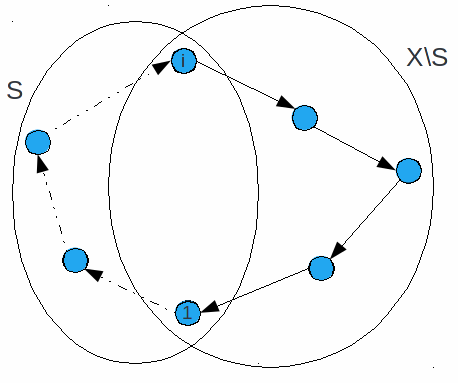
\includegraphics[height=4cm]{images/graph50.png} &
		\begin{equation*}
			f(S,i)+f'(X\setminus S,i)=z^{*}
		\end{equation*}
	\end{tabular}
\end{table}
Sia $z_{UB}$ un upper bound a $z^{*}$ calcolato con un euristico. Sia $k=|S|$ per cui $|X\setminus S|=n-k$.

Lo stato $(S,i)$ non può far parte del $TSP$ ottimo se:
\begin{equation*}
	f(S,i)+
	\begin{cases}
		f'(n-k,i),\ \textnormal{se }\pi'(n-k,i)\notin S \\
		\phi'(n-k,i)\ \textnormal{se }\pi'(n-k,i)\in S
	\end{cases}
	\ge z_{UB}
\end{equation*}

\subsection{Algoritmo di programmazione dinamica per il TSP}
\begin{enumerate}
	\item Poni $\mathscr{L}_{i}\{(\{i\}),1\}$, $f(\{i\},1)=0$, $p(\{i\},1)=1$ e $\mathscr{L}_{r}=\emptyset$, $r=2,\dots,n$. Sia $z_{UB}$ un upper bound al $TSP$. Poni $k=2$;
	\item Espandi ogni stato del set $\mathscr{L}_{k-1}$:\\
	per ogni $(S,i)\in\mathscr{L}_{k-1}$ ripeti lo step 3;
	\item Genera gli stati di $\mathscr{L}_{k}$ raggiungibili da $(S,i)$:\\
	per ogni $j\in\Gamma^{-1}\setminus S$ considera lo stato $(S',j)$ dove $S'=S\cup\{j\}$. Poni $h=f(S,i)+c_{ij}$.\\
	Lo stato $(S',j)$ deve essere "rigettato" nei seguenti casi:
	\begin{itemize}
		\item se $h+f'(n-k,i)\ge z_{UB}$ qualora $\pi'(n-k,i)\notin S'$;
		\item se $h+\phi'(n-k,j)\ge z_{UB}$ qualora $\pi'(n-k,j)\in S'$;
		\item se $(S',j)\in\mathscr{L}_{k}$ e $f(S',j)\le h$.
	\end{itemize}
	Se $(S',j)\notin\mathscr{L}_{k}$ allora poni $\mathscr{L}_{k}=\mathscr{L}_{k}\cup\{(S',j)\}$, $f(S',j)=h$ e $p(S',j)=(S,i)$.\\
	Se $(S',j)\in\mathscr{L}_{k}$ e $f(S',j)>h$ allora poni $f(S',j)=h$ e $p(S',j)=(S,i)$;
	\item Poni $k=k+1$; se $k\le n$ vai allo step 2;
	\item L'ottimo è dato da $z^{*}=\underset{(X,j)\in\mathscr{L}_{k}}{Min}[f(X,j)+c_{j1}]$.
\end{enumerate}

%\include{cap_6}
%\chapter{Metodi di decomposizione}

\section{Dantizg-Wolfe Decomposition}
Si consideri il seguente problema di programmazione lineare:
\begin{equation*}
	(P)
	\begin{cases}
		Min\ cx \\
		\ \ \ \ \ \ Ax=b \\
		\ \ \ \ \ \ x\in X
	\end{cases}
	A\textnormal{ è ($m$ x $n$)}
\end{equation*}
dove $X$ è un insieme \textit{poliedrico convesso limitato} che rappresenta vincoli aventi una "speciale" struttura.

Per il teorema della rappresentazione, essendo per ipotesi $X$ un insieme limitato, detti $x^{1},x^{2},\dots,x^{t}$ i punti estremi di $X$ allora ogni $x\in X$ può essere rappresentato come:
\begin{flalign*}
	& x=\sum_{j=1}^{t}\lambda_{j}x^{j} \\
	& s.t.\ \sum_{j=1}^{t}\lambda_{j}=1 \\
	& \ \ \ \ \ \lambda_{j}\ge 0,\ j=1,\dots,t
\end{flalign*}
Sostituendo $x$ così definito in $P$ si ottiene la seguente formulazione equivalente di $P$ nelle variabili $\lambda_{1},\lambda_{2},\dots,\lambda_{t}$.

\begin{numcases}{P'}
	z'=Min\ \sum_{j=1}^{t}(cx^{j})\lambda_{j} \\
	\ \ \ \ \ \ \ \ s.t.\ \sum_{j=1}^{t}(Ax^{j})\lambda_{j}=b \label{eq:5.2} \\
	\ \ \ \ \ \ \ \ \ \ \ \ \ \ \sum_{j=1}^{t}\lambda_{j}=1 \label{eq:5.3} \\
	\ \ \ \ \ \ \ \ \ \ \ \ \ \ \lambda\ge 0,\ j=1,\dots,t
\end{numcases}

\subsection{Metodo di soluzione di $\boldsymbol{P'}$}
$P'$ non può essere risolto direttamente poichè il numero $t$ di punti estremi di $X$ è (di solito) molto grande e tali punti non possono essere enumerati a priori.

Si cerca quindi di risolvere $P'$ senza dover generare tutti i punti estremi di $X$.

\clearpage
\subsubsection{Schema dell'algoritmo}
\begin{enumerate}
	\item \textbf{Problema Master}
		\begin{itemize}
			\item Si risolva $P'$ usando un insieme limitato di $k$ punti estremi $x^{1},\dots,x^{k}$ dove $k\ll t$.
			\item Sia $(w,\alpha)$ la soluzione duale ottima di $P'$ usando i $k$ punti estremi generati.\\
			$w=(w_{1},w_{2},\dots,w_{t})$ variabile duale dei vincoli \ref{eq:5.2} e $\alpha$ variabile duale del vincolo \ref{eq:5.3}.
			\begin{equation*}
				D'
				\begin{cases}
					Max\ w b+\alpha \\
					\ \ s.t.\ w(Ax^{j})+\alpha\le cx^{j},\ j=1,\dots,k \\
					\ \ \ \ \ \ \ w\in\mathscr{R}^{m},\ \alpha\in\mathscr{R} \\
				\end{cases}
			\end{equation*}
		\end{itemize}
	\item \textbf{Ottimalità della soluzione del Master $\boldsymbol{P'}$}\\
	La soluzione ottima di $P'$ è ottima per l'intero problema se e solo se $(w,\alpha)$ soddisfa i vincoli duali dei punti estremi $x^{k+1},x^{k+2},\dots,x^{t}$ non considerati di $P'$, ovvero:
	\begin{equation*}
		w(Ax^{j})+\alpha\le cx^{j},\ j=k+1,\dots,t
	\end{equation*}
	In altri termini, la soluzione di $P'$ è ottima e $(w,\alpha)$ è ottima per $D'$ se
	\begin{equation}
		z_{j}-c_{j}=w(Ax^{j})+\alpha-cx^{j}=(w A-c)x^{j}+\alpha\le 0,\ j=k+1,\dots,t \label{eq:5.5}
	\end{equation}
	Per verificare se le \ref{eq:5.5} sono soddisfatte o violate è sufficiente cercare (se esiste) il punto estremo di $X$ che viola le \ref{eq:5.5}.\\
	Tale punto estremo, se esiste, sarà la soluzione ottima di costo positivo del seguente sottoproblema $SP$:
	\begin{equation*}
		SP
		\begin{cases}
			z_{SP}=Max\ (w A-c)x+\alpha \\
			\ \ \ \ \ \ \ \ \ s.t.\ \ x\in X
		\end{cases}
	\end{equation*}
	sia $x^{*}$ la soluzione ottima di $SP$
	\item Se $z_{SP}>0$ allora la corrente soluzione duale $(w,\alpha)$ viola il vincolo \ref{eq:5.5} per il punto estremo $x^{*}$ di $X$.
	
	Poni $k=k+1$, $x^{k}=x^{*}$ e ritorna allo step 1.\\
	Se $z_{SP}=0$ allora $(w,\alpha)$ soddisfa i vincoli duali \ref{eq:5.5} per i punti estremi non considerati da $P'$, quindi la soluzoine di $P'$ è ottima: \textit{stop}.
\end{enumerate}
Potrebbe risultare computazionalmente proibitivo raggiungere la condizione di ottimalità a causa dell'evelato numero di punti estremi.

\clearpage
\subsection{Lower Bound}
Ad ogni interazione è possibile calcolare un lower bound $LB$ al costo ottimo $z^{*}$ di $P$ e quindi si può terminare l'algoritmo quando il costo di $z'$ di $P'$ limitato a $k$ punti estremi è sufficientemente "vicino" a $LB$; ad esempio, quando
\begin{equation}
	\frac{z'-LB}{LB}\le TOL \label{eq:5.6}
\end{equation}
dove $TOL$ è definito a-priori dall'utente.
\subsubsection{Calcolo del lower bound $\boldsymbol{LB}$}
Si noti che per come è definito $SP$ si ha che
\begin{equation*}
	(w A-c)x+\alpha\le z_{SP},\ \forall x\in X
\end{equation*}
o anche
\begin{equation}
	w Ax-cx+\alpha\le z_{SP}, \ \forall x\in X \label{eq:5.7}
\end{equation}
Si consideri una qualunque soluzione $x$ di $P$ (ovvero $x\in X$ e $Ax=b$), dalla \ref{eq:5.7} si ha:
\begin{equation*}
	w b-cx+\alpha\le z_{SP}
\end{equation*}
o anche
\begin{equation*}
	cx\ge\overbrace{w b+\alpha}^{z'}-z_{SP}=z'-z_{SP}
\end{equation*}
Qunidi $LB=w b+\alpha-z_{SP}$ è un lower bound valido e l'algoritmo può terminare qualora la soluzione $z'$ del problema master verifichi la \ref{eq:5.6}.

\subsection{Esempio}
\begin{flalign*}
		& Min\ -2x_{1}-x_{2}-x_{3}+x_{4} \\
		& s.t. \ \ \begin{rcases}
					x_{1}+x_{3}\le 2 \\
					x_{1}+x_{2}+2x_{4}\le 3  \\
			   \end{rcases} Ax\le b \\
		& \ \ \ \ \ \ \ \begin{rcases}
				   x_{1}\le 2 \\
				   x_{1}+2x_{2}\le 5 \\
				   -x_{3}+x_{4}\le 2 \\
				   2x_{3}+x_{4}\le 6 \\
				   x_{1},x_{2},x_{3},x_{4}\ge 0
			   \end{rcases}x\in X
\end{flalign*}
Quindi, formalmente, $P$ può essere scritto come
\begin{equation*}
	P
	\begin{cases}
		Min\ cx \\
		\ \ \ \ \ \ \ Ax+s=b \\
		\ \ \ \ \ \ \ x\in X, s\ge 0 \ x\ge 0
	\end{cases}
\end{equation*}
Ogni $(x_{1},x_{2},x_{3},x_{4})\in X$ ha le prime due componenti in $X_{1}$ e le ultime due in $X_{2}$ come mostrato in seguito.\\
\centerline{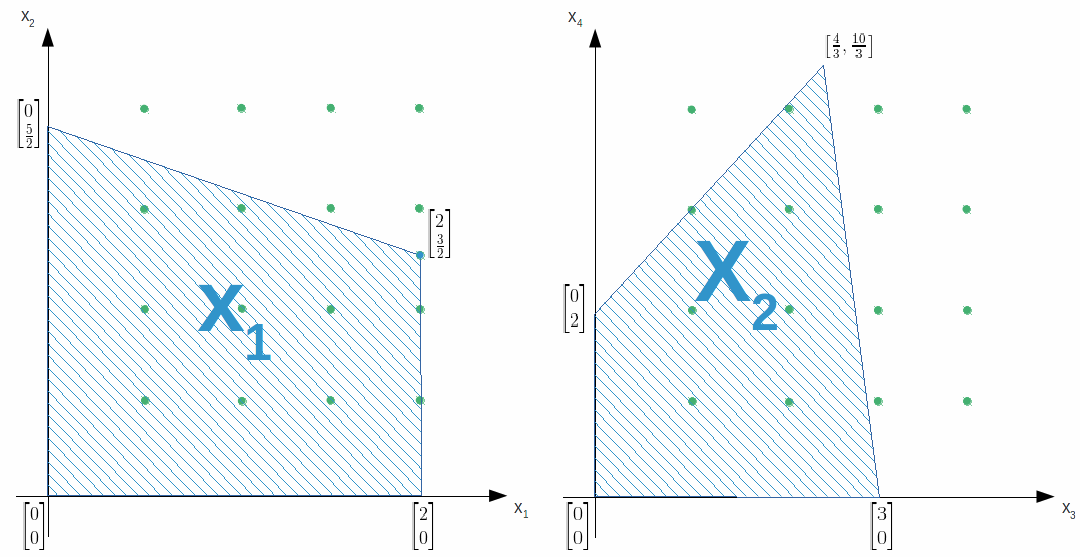
\includegraphics[height=7cm]{images/graph51.png}\label{fig:5.1.3}}\\
\begin{flalign*}
	& X_{1}=\{(x_{1},x_{2}):x_{1}\le 2, x_{1}+2x_{2}\le 5; \ x_{1},x_{2}\ge 0\} \\
	& X_{2}=\{(x_{3},x_{4}):-x_{3}+x_{4}\le 2,\ 2x_{3}+x_{4}\le 6,\ x_{3},x_{4}\ge 0\}
\end{flalign*}
\subsection{Inizializzazione}
Siano $x^{1},x^{2},\dots,x^{t}$ i punti estremi di $X$.\\
Poniamo $\hat{c}_{j}=cx^{j}$ il costo del punto estremo $x^{j}$, $j=1,\dots,t$
\begin{equation*}
	P'
	\begin{cases}
		Min\ \sum_{j=1}^{t}\hat{c}_{j}\lambda_{j} \\
		\ \ \ \ \ \ \ \sum_{j=1}^{t}(Ax^{j})\lambda_{j}+s=b \\
		\ \ \ \ \ \ \ \sum_{j=1}^{t}\lambda_{j}=1 \\
		\ \ \ \ \ \ \ \lambda_{j}\ge 0,\ j=1,\dots,t
	\end{cases}
\end{equation*}
\clearpage
Si può partire con il punto estremo $x^{1}=(0,0,0,0)$ di costo $\hat{c}_{1}=0$
\begin{equation*}
	P'
	\begin{cases}
		z^{1}=Min\ 0\lambda_{1} \\
		\ \ \ \ \ \ \ \ \ s_{1}=2\ \ \ \ \ \ \ \ \ \ \ \ w_{1}\\
		\ \ \ \ \ \ \ \ \ s_{2}=3\ \ \ \ \ \ \ \ \ \ \ \ w_{2}\\
		\ \ \ \ \ \ \ \ \ \lambda_{1}=1\ \ \ \ \ \ \ \ \ \ \ \ \alpha\\
		\ \ \ \ \ \ \ \ \ s_{1},s_{2},\lambda_{1}\ge 0
	\end{cases}
\end{equation*}
Ottimo: $\lambda_{1}=1$, $s_{1}=2$, $s_{2}=3$, $z^{1}=0$ e $(w_{1},w_{2},\alpha)=(0,0,0,0)$.\\

La soluzione primale di $P$ di costo $z^{1}=0$ è $x=\lambda_{1}x^{1}=0x^{1}=(0,0,0,0)$.

\subsubsection{Iterazione 1}
\begin{equation*}
	SP
	\begin{cases}
		Max\ \ (w A-c)x+\alpha \\
		\ \ \ \ \ \ \ \ \ s.t. \ x\in X
	\end{cases}
\end{equation*}
Poichè $(w_{1},w_{2},\alpha)=0$

\begin{flalign*}
& SP\ \ \ \ \ \ \ \ \ Max\ 2x_{1}+x_{2}+x_{3}-x_{4}+0 \\
& \ \ \ \ \ \ \ \ \ \ \ \ \ \ \ \ \ \ \ \ \ x\in X \textnormal{ o }(x_{1},x_{2})\in X_{1},\ (x_{3},x_{4})\in X_{2}
\end{flalign*}

$SP$ è separabile nei vettori $(x_{1},x_{2})\in X_{1}$ e $(x_{3},x_{4})\in X_{2}$ per cui, come si vede in \ref{fig:5.1.3}, si ha che una soluzione ottima di $SP$ è data dal punto estremo

\begin{equation*}
	x^{2}=(2,\frac{3}{2},3,0)
\end{equation*}

$z_{2}-\hat{c}_{2}=(w A-c)x^{2}+\alpha=-cx^{2}=\frac{17}{2}>0$

Lower bound $z^{1}-(z_{2}-\hat{c}_{2})=-\frac{17}{2}=-8.5$ e $x_{2}$ entra nel Master

\clearpage
\subsubsection{Nuovo Master}
\begin{equation*}
	P'
	\begin{cases}
		Min\ \ \hat{c}_{1}\lambda_{1}+\hat{c}_{2}\lambda_{2}\\
		\ \ \ \ \ \ \ (Ax^{1})\lambda_{1}+(Ax_{2})\lambda_{2}+s=b \\
		\ \ \ \ \ \ \ \ \ \ \ \ \ \ \ \lambda_{1}+\lambda_{2}=1 \\
		\ \ \ \ \ \ \ \ \ \ \ \ \ \ \ \lambda_{1}+\lambda_{2}\ge 0,\ s\ge 0
	\end{cases}
\end{equation*}
Nel calcolo in esame $Ax^{1}=\begin{bmatrix}0\\0\end{bmatrix}$, $Ax_{2}=\begin{bmatrix}5\\\frac{7}{2}\end{bmatrix}$, quindi
\begin{equation*}
	P'
	\begin{cases}
		z^{1}=Min\ 0\cdot\lambda_{1}+(-\frac{17}{2})\lambda_{2} \\
		\ \ \ \ \ \ \ \ \ \ \ \ \ \ 0\cdot\lambda_{1}+5\lambda_{2}+s_{1}=2 \\
		\ \ \ \ \ \ \ \ \ \ \ \ \ \ 0\cdot\lambda_{1}+\frac{7}{2}\lambda_{2}+s_{2}=3 \\
		\ \ \ \ \ \ \ \ \ \ \ \ \ \ \lambda_{1}+\lambda_{2}=1 \\
		\ \ \ \ \ \ \ \ \ \ \ \ \ \ \lambda_{1},\lambda_{2},s_{1},s_{2}\ge 0
	\end{cases}
\end{equation*}
Ottimo: $\lambda_{1}=\frac{3}{5}$, $\lambda_{2}=\frac{2}{5}$, $s_{1}=0$, $s_{2}=\frac{2}{5}$, $z^{1}=-\frac{17}{5}$.
\begin{equation*}
	(w_{1},w_{2},\alpha)=(-\frac{17}{10},0,0)
\end{equation*}
La soluzione primale di $P$ di costo $z^{1}=-\frac{17}{6}=-3\cdot 4$ è
\begin{equation*}
	x=\lambda_{1}x^{1}+\lambda_{2}x^{2}=\frac{5}{3}+\frac{2}{5}x^{2}=(\frac{4}{5},\frac{3}{5},\frac{6}{5},0)
\end{equation*}

\subsubsection{Iterazione 2}
\begin{equation*}
	SP
	\begin{cases}
		Max\ \ (w A-c)x+\alpha \\
		\ \ \ \ \ \ \ \ \ s.t. \ x\in X
	\end{cases}
\end{equation*}
$(w A-c)=(\frac{3}{10},1,-\frac{7}{10},-1)$
\begin{equation*}
	SP
	\begin{cases}
		Max\ \frac{3}{10}x_{1}+x_{2}-\frac{7}{10}x_{3}-x_{4}+0 \\
		\ \ \ \ \ \ \ \ s.t.\ (x_{1},x_{2})\in X_{1},\ (x_{3},x_{4})\in X_{2}
	\end{cases}
\end{equation*}
Ottimo $x^{3}=(0,\frac{5}{2},0,0)$ e $z-\hat{c}_{3}=\frac{5}{2}>0$.\\
Lower bound $z^{1}-(z_{3}-\hat{c}_{3})=-\frac{17}{5}-\frac{5}{2}=-5.4$

\subsubsection{Nuovo Master}
\begin{equation*}
	P'
	\begin{cases}
		Min\ \hat{c}_{1}\lambda_{1}+\hat{c}_{2}\lambda_{2}+\hat{c}_{3}\lambda_{3}\\
		\ \ \ \ \ \ \ (Ax^{1})\lambda_{1}+(Ax^{2})\lambda_{2}+(Ax^{3})\lambda_{3}+s=b \\
		\ \ \ \ \ \ \ \lambda_{1}+\lambda_{2}+\lambda_{3}=1 \\
		\ \ \ \ \ \ \ \lambda_{1},\lambda_{2},\lambda_{3},s\ge 0
	\end{cases}
\end{equation*}
$\hat{c}_{3}=cx^{3}=-\frac{5}{2}$, $Ax^{3}=\begin{Bmatrix}0\\\frac{5}{2}\end{Bmatrix}$, quindi
\begin{equation*}
	P'
	\begin{cases}
		z^{1}=Min\ 0\cdot\lambda_{1}-\frac{17}{2}\lambda_{2}-\frac{5}{2}\lambda_{3} \\
		\ \ \ \ \ \ \ \ \ \ \ \ \ \  0\cdot\lambda_{1}+5\lambda_{2}+0\cdot\lambda_{3}+s_{1}=2 \\
		\ \ \ \ \ \ \ \ \ \ \ \ \ \  0\cdot\lambda_{1}+\frac{7}{2}\lambda_{2}+\frac{5}{2}\lambda_{3}+s_{2}=3 \\
		\ \ \ \ \ \ \ \ \ \ \ \ \ \ \lambda_{1}+\lambda_{2}+\lambda_{3}=1
	\end{cases}
\end{equation*}
Ottimo: $\lambda_{1}=0$, $\lambda_{2}=\frac{2}{5}$, $\lambda_{3}=\frac{3}{5}$, $s_{1}=0$, $s_{1}=\frac{1}{10}$ e $z^{1}=-4.9$, inoltre, $(w_{1},w_{2},\alpha)=(-\frac{6}{5},0,-\frac{5}{2})$.\\
Lo soluzione di $P$ di costo $-4.9$ è $x=\lambda_{2}x^{2}+\lambda_{3}x^{3}=(\frac{4}{5},21,\frac{6}{5},0)$

\subsubsection{Iterazione 3}
\begin{equation*}
	SP
	\begin{cases}
		Max\ (w A-c)x+\alpha \\
		\ \ \ \ \ \ \ \ s.t.\ x\in X
	\end{cases}
\end{equation*}
$(w A-c)=(\frac{4}{5},1,-\frac{1}{5},-1)$
\begin{equation*}
	SP
	\begin{cases}
		z_{SP}=Max\ \frac{4}{5}x_{1}+x_{2}-\frac{1}{5}x_{3}-x{4}-\frac{5}{2} \\
		\ \ \ \ \ \ \ \ (x_{1},x_{2})\in X_{1},\ (x_{3},x_{4})\in X_{2}
	\end{cases}
\end{equation*}
$x^{4}=(2,\frac{3}{2},0,0)$ e $z_{SP}=(z_{4}-\hat{c}_{4})=\frac{3}{5}$.\\
Lower Bound $z^{1}-(z_{4}-\hat{c}_{4})=-4.9-\frac{3}{5}=-5.5$

\subsubsection{Nuovo Master}
\begin{flalign*}
	& Ax^{4}=\begin{Bmatrix}2\\\frac{7}{2}\end{Bmatrix} \\
	& cx^{4}=-\frac{11}{2}
\end{flalign*}
\begin{equation*}
	P
	\begin{cases}
		z^{1}=Min\ 0\cdot\lambda_{1}-\frac{17}{2}\lambda_{2}-\frac{5}{2}\lambda_{3}-\frac{11}{2}\lambda_{4} \\
		\ \ \ \ \ \ \ \ \ \ \ \ \ \ 0\cdot\lambda_{1}+5\lambda_{2}+0\cdot\lambda_{3}+2\lambda_{4}+s_{1}=2 \\
		\ \ \ \ \ \ \ \ \ \ \ \ \ \ 0\cdot\lambda_{1}+\frac{7}{2}\lambda_{2}+\frac{6}{2}\lambda_{3}+\frac{7}{2}\lambda_{4}+s_{2}=3 \\
		\ \ \ \ \ \ \ \ \ \ \ \ \ \ \lambda_{1}+\lambda_{2}+\lambda_{3}+\lambda_{4}=1 \\
		\ \ \ \ \ \ \ \ \ \ \ \ \ \ \lambda_{1},\dots,\lambda_{4},s_{1},s_{2}\ge 0
	\end{cases}
\end{equation*}
Ottimo $\lambda_{1}=0$, $\lambda_{2}=\frac{1}{3}$, $\lambda_{3}=\frac{1}{6}$, $\lambda_{4}=\frac{1}{2}$, $z^{1}=-5$.

$(w_{1},w_{2},\alpha)=(-1,-1,0)$

La soluzione di $P$ di costo $-$ è $x=\lambda_{2}x^{2}+\lambda_{3}x^{3}+\lambda_{4}x^{4}=\frac{1}{3}x^{2}+\frac{1}{6}x_{3}+\frac{1}{2}x^{4}=(1,2,1,0)$

\subsubsection{Iterazione 4}
\begin{equation*}
	SP
	\begin{cases}
		Max\ (w A-c)x+\alpha \\
		\ \ \ \ \ \ \ x\in X
	\end{cases}
\end{equation*}
$(w A-c)=(0,0,0,-3)$
\begin{equation*}
	SP
	\begin{cases}
		z_{SP}=Max\ 0\cdot x_{1}+0\cdot x_{2}+0\cdot x_{3}-3x_{4}+0 \\
		\ \ \ \ \ \ \ \ (x_{1},x_{2})\in X_{1},\ (x_{3},x_{4})\in X_{2} 
	\end{cases}
\end{equation*}
Ottimo $z_{SP}=0$: \textit{stop}.

Lower Bound $z^{1}-z_{SP}=z^{1}=-s$.

Quindi la soluzione ottima del problema originario è
\begin{equation*}
	x=\frac{1}{3}x^{2}+\frac{1}{6}x^{3}+\frac{1}{2}x^{4}=(1,2,1,0)
\end{equation*}
\centerline{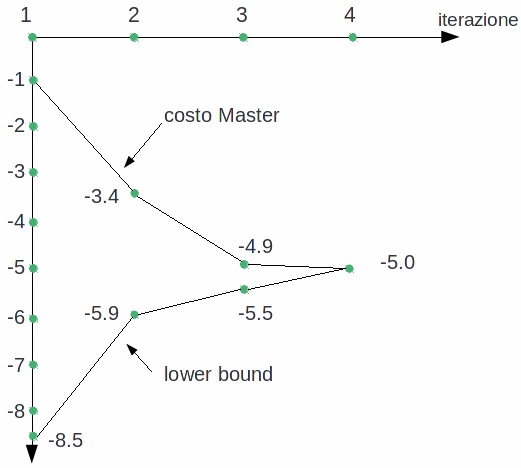
\includegraphics[height=7cm]{images/graph52.png}}

\section{Struttura Diagonale a blocchi di X}
È il caso in cui $X$ può essere decomposto in $T$ sottoinsiemi $X_{1},X_{2},\dots,X_{T}$ e il vettore delle varibili in $T$ vettori $x_{1},x_{2},\dots,x_{T}$ tali che $x_{k}\in X_{k}$, $k=1,\dots,T$.\\
Indichiamo con $c_{k}$ il vettore dei costi e con $A_{k}$ la sottomatrice di $A$ relativa alle variabili $x_{k}$, $k=1,\dots,T$.\\
Il problema $P$ si può scrivere come seuge:
\begin{equation*}
	P
	\begin{cases}
	Min\ c_{1}x_{1}+c_{2}x_{2}+\dots+c_{T}x_{T}=Min\ \sum_{k=1}^{T}c_{k}X_{k} \\
	\ \ \ \ \ \ \ A_{1}x_{1}+A_{2}x_{2}+\dots+a_{T}x_{T}=b\ \sum_{k}A_{k}x_{k}=b \\
	\ \ \ \ \ \ \ B_{1}x_{1}\ \ \ \ \ \ \ \ \ \ \ \ \ \ \ \ \ \ \ \ \ \ \ \ \ \ \ \ =b_{1} \\
	\ \ \ \ \ \ \ \ \ \ \ \ \ \ \ \ \ B_{2}x_{2}\ \ \ \ \ \ \ \ \ \ \ \ \ \ \ \ \ \ =b_{2} \\
	\ \ \ \ \ \ \ \ \ \ \ \ \ \ \ \ \ \ \ \ \ \ \ \ \ \ \ \ddots\ \ \ \ \ \ \ \ \ \ \ \ \ \vdots \\
	\ \ \ \ \ \ \ \ \ \ \ \ \ \ \ \ \ \ \ \ \ \ \ \ \ \ \ \ \ \ \ \ \ \ B_{T}x_{T}=b_{T}\\
	\ \ \ \ \ \ \ x_{1},x_{2},\dots,x_{T}\ge 0
	\end{cases}
\end{equation*}
dove $X_{i}=\{x_{i}:B_{i}x_{i}=b_{i},\ x_{i}\ge 0\}$, $i=1,\dots,T$.\\
L'algoritmo descritto in precedenza può essere ulteriormente specializzato per sfruttare la particolare struttura che definisce $x\in X$.

Supponiamo che ogni insieme $X_{i}$ sia limitato.\\
Per ogni sottoinsieme $X_{k}$ (limitato) indichiamo con $x^{1}_{k},x^{2}_{k},\dots,x^{t_{k}}_{k}$ i punti estremi, quindi $x_{k}\in X_{k}$ può essere rappresentato come
\begin{equation*}
	\begin{rcases}
		x_{k}=\sum_{j=1}^{t_{k}}\lambda_{kj}x_{k}^{j}\ \ \ \ \ \ \ \ \ \ \ \ \ \ \ \ \ \ \ \ \ \\
		\sum_{j=1}^{t_{k}}\lambda_{kj}=1\ \ \ \ \ \ \ \ \ \ \ \ \ \ \ \ \ \ \ \\
		\lambda_{kj}\ge 0,\ j=1,\dots,t_{k}
	\end{rcases}
	k=1,\dots,T
\end{equation*}
Sostituendo ogni $x_{k}$ con $k=1,\dots,T$ così definito in $P$ si ha
\begin{numcases}{P'}
	z'=Min\ \sum_{k=1}^{T}(\sum_{j=1}^{t_{k}}(c_{k}x_{k}^{j})\lambda_{kj}) \\
	\ \ \ \ \ \ \ \ \ \ \ \ \ \ \sum_{k=1}^{T}(\sum_{j=1}^{t_{k}}(A_{k}x_{k}^{j})\lambda_{kj})=b \label{eq:5.9}\\
	\ \ \ \ \ \ \ \ \ \ \ \ \ \ \sum_{j=1}^{t_{k}}\lambda_{kj}=1,\ k=1,\dots,T \label{eq:5.10}\\
	\ \ \ \ \ \ \ \ \ \ \ \ \ \ \lambda_{kj}\ge 0,\ j=1,\dots,t_{k},\ k=1,\dots,T
\end{numcases}
Siano $w=(w_{1},\dots,w_{m})$ e $\alpha=(\alpha_{1},\dots,\alpha_{T})$ le variabili duali, rispettivamente dei vincoli \ref{eq:5.9} e \ref{eq:5.10}.
\begin{equation*}
	D'
	\begin{cases}
		Max\ w b+\sum_{k=1}^{T}\alpha_{k} \\
		\ \ \ \ \ \ \ \ w(A_{k}x_{k}^{j})+\alpha_{k}\le c_{k}x_{k}^{j},\ j=1,\dots,t_{k},\ k=1,\dots,T \\
		\ \ \ \ \ \ \ \ w\in\mathscr{R}^{m},\ \alpha\in\mathscr{R}^{T}
	\end{cases}
\end{equation*}

\subsection{Metodo di soluzione}
Si fa uso della particolare struttura di $X$.
\begin{enumerate}
	\item \textbf{Master problem}\\
	Si risolva $P'$ usando un numero limitato $r_{k}\ll t_{k}$ dei punti estremi di ciascun insieme $X_{k}$, $k=1,\dots,T$.\\
	Sia $(w,\alpha)$ la soluzione del duale del suddetto master.
	\item \textbf{Ottimalità della soluzione del Master}\\
	La soluzione del Master è ottima se $(w,\alpha)$ soddisfa i vincoli duali per i punti estremi non generati; ovvero, se per ogni $k=1,\dots,T$
	\begin{equation*}
		w(A_{k}x_{k}^{j})+\alpha_{k}\le c_{k}x_{k}^{j},\ j=r_{k}+1,\dots,t_{k}
	\end{equation*}
	ovvero se
	\begin{equation*}
			(w A_{k}-c_{k})x_{k}^{j}+\alpha_{k}\le 0,\ j=r_{k}+1,\dots,t_{k}
	\end{equation*}
	Si risolva quindi per ogni $k=1,\dots,T$
	\begin{equation*}
		SP_{k}
		\begin{cases}
			z_{SP}=Max\ (w A_{k}-c_{k})x_{k}+\alpha_{k} \\
			\ \ \ \ \ \ \ \ \ \ \ s.t.\ B_{k}x_{k}=b_{k} \\
			\ \ \ \ \ \ \ \ \ \ \ \ \ \ \ \ \ x_{k}\ge 0
		\end{cases}
	\end{equation*}
	Sia $x_{k}^{*}$ la soluzione ottima.
	\item Se $z_{SP}^{k}\ge 0$, $\forall k:\ stop$ la soluzione è ottima; altrimenti per ogni $k$ per cui $z_{SP}^{k}>0$ poni $r_{k}=r_{k}+1$, $x_{k}^{r_{k}}=x_{k}$ e quindi ritorna al punto 1.
\end{enumerate}

\clearpage
\subsection{Lower Bound}
Come descritto in precedenza, si può terminare l'algoritmo quando il costo $z'$ del Master non dista "troppo" dall'ottimo ovvero quando
\begin{equation*}
	\frac{z'-LB}{LB}\le TOL
\end{equation*}
dove $LB$ può essere così calcolato.
Per come è definito ogni $SP_{k}$, $k=1,\dots,T$, si ha che
\begin{equation*}
	(w A_{k}-c_{k})x_{k}+\alpha_{k}\le z_{SP}^{k},\ k=1,\dots,T
\end{equation*}
o anche
\begin{equation*}
	c_{k}x_{k}\ge w A_{k}x_{k}+\alpha_{k}-z_{SP}^{k},\ k=1,\dots,T
\end{equation*}
sommando
\begin{equation*}
	\sum_{k=1}^{T}c_{k}x_{k}\ge w\sum_{k=1}^{T}A_{k}x_{k}+\sum_{k=1}^{T}\alpha_{k}-\sum_{k=1}^{T}z_{SP}^{k}
\end{equation*}

Si consideri un qualunque $x=(x_{1},...,x_{T})$ che soddisfi $x_{k}\in X_{k}$, $\forall k$ e $A_{1}x_{1}+A_{2}x_{2}+\dots,A_{T}x_{T}=b$ si ha
\begin{equation*}
	\sum_{k=1}^{T}c_{k}x_{k}\ge w b+\sum_{k=1}^{T}\alpha_{k}-\sum_{k=1}^{T}z_{SP}^{k}
\end{equation*}
Quindi $LB=\underbrace{w b+\sum_{k}\alpha_{k}}_{z'}-\sum_{k}z^{k}_{SP}$.

$LB$ è un limite inferiore al costo della soluzione ottima.

\section{Assegnamento Generalizzato}
\begin{itemize}
	\item[m] contenitori di capacità $Q_{1},\dots,Q_{m}$
	\item[n] oggetti che devono essere caricati nei contenitori
	\item[$c_{ij}$] costo per caricare l'oggetto $i$ nel contenitore $j$
	\item[$q_{ji}$] spazio del contenitore $j$ occupato da $i$ se $i$ viene caricato nel contenitore $j$.
\end{itemize}
Si vogliono caricare tutti gli oggetti nei contenitori minimizzando il costo complessivo.
\begin{numcases}{P}
	Min\ \,\sum_{i=1}^{n}\sum_{j=1}^{m}c_{ij}x_{ij} \label{eq:5.12}\\
	\ \ s.t.\ \sum_{j=1}^{m}x_{ij}=1,\ i=1,\dots,n \label{eq:5.13} \\
	\ \ \ \ \ \ \ \ \sum_{i=1}^{n}q_{ij}x_{ij}\le Q,\ j=1,\dots,m \label{eq:5.14}\\
	\ \ \ \ \ \ \ \ \ \ \ \ \ x_{ij}\in\{0,1\},\ \forall i,j \label{eq:5.15}
\end{numcases}
$x_{ij}=1$ se $i$ è caricato nel contenitore $j$; $x_{ij}=0$ altrimenti.

\subsection{Decomposizione Dantzig-Wolfe del GAP}
Indichiamo con $X_{j}$ l'insieme delle soluzioni intere del vincolo \ref{eq:5.14} per il contenitore $j$, $j=1,\dots,m$
\begin{equation*}
	X_{j}=\{x_{j}:\sum_{i=1}^{n}q_{ij}x_{ij}\le Q,\ x_{ij}\in\{0,1\},\ i=1,\dots,n\}
\end{equation*}
dove $x_{j}=(x_{1j},x_{2j},\dots,x_{nj})^{T}$.\\
Siano $x_{j}^{1},x_{j}^{2},\dots,x_{j}^{t_{j}}$ i punti estremi di $conv(X_{j})$.

Per il teorema della rappresentazione abbiamo:
\begin{flalign}
	& \begin{rcases} \label{eq:5.16}
		x_{ij}=\sum_{r=1}^{t_{j}}\lambda_{jr}x_{ij}^{r},\ i=1,\dots,m \\
		\sum_{r=1}^{t_{j}}\lambda_{jr}=1\ \ \ \ \ \ \ \ \ \ \ \ \ \ \ \ \,\\
		\lambda_{jr}\ge 0\ \ \ \ \ \ \ \ \ \ \ \ \ \ \ \ 
	  \end{rcases} j=1,\dots,m
\end{flalign}
Sostituendo in $P$, definito da \ref{eq:5.12} - \ref{eq:5.15}, $x_{ij}$ secondo \ref{eq:5.16}:
\begin{numcases}{P'}
	Min\ \sum_{i=1}^{n}\sum_{j=1}^{m}c_{ij}\sum_{r=1}^{t_{j}}\lambda_{jr}x_{ij}^{r} \\
	\ \ s.t.\ \sum_{j=1}^{m}\sum_{r=1}^{t_{j}}\lambda_{jr}x_{ij}^{r}=1,\ i=1,\dots,n \\
	\ \ \ \ \ \ \ \ \sum_{r=1}^{t_{j}}\lambda_{jr}=1,\ j=1,\dots,m \\
	\ \ \ \ \ \ \ \ \ \ \ \ \ \lambda_{jr}\in\{0,1\},\ j=1,\dots,m,\ r=1,\dots,t_{j} \label{eq:5.20}
\end{numcases}
I vincoli \ref{eq:5.20} derivano dal fatto che $x_{ij}\in\{0,1\}$.\\

Perché $\lambda_{ji}\in\{0,1\}$ invece di $\lambda_{jr}\ge 0$?

Il motivo è che le soluzioni frazionarie di $\lambda_{jr}$ per un dato $j$ inducono nei \ref{eq:5.20} soluzioni frazionarie di $x_{ij}$.\\
Si consideri il sequente esempio dei \ref{eq:5.20} per un dato $j$ per il quale vengono mostrati $t_{j}=5$ punti estremi di $conv(X_{j})$.
\begin{table}[!h]
	\centering
	\begin{tabular}{c|cccccc}
		& $\lambda_{j1}$ & $\lambda_{j2}$ & $\lambda_{j3}$ & $\lambda_{j4}$ & $\lambda_{j5}$ \\ \cline{1-6}
		$x_{1j}$ & 1 & 1 & 0 & 0 & 1 & \\
		$x_{2j}$ & 0 & 1 & 1 & 0 & 1 & \\
		$\cdot$  & 1 & 0 & 1 & 1 & 0 & \\
		$\cdot$  & 0 & 1 & 0 & 1 & 0 & \\
		$\cdot$  & 1 & 0 & 0 & 1 & 0 & \\
		$x_{6j}$ & 0 & 0 & 1 & 0 & 1 & \\
		& 1 & 1 & 1 & 1 & 1 & = 1
	\end{tabular}
\end{table}
\begin{equation*}
	\lambda_{j1},\dots,\lambda_{j5}\ge 0
\end{equation*}
Ogni soluzione frazionaria di $\lambda$ induce una soluzione frazionaria in $x_{ij}$.

\textbf{Esempio.}

$\lambda_{ji}=\frac{1}{2}$, $\lambda_{j2}=\frac{1}{2}$ e $\lambda_{j3}=\lambda_{j4}=\lambda_{j5}=0$

induce

$x_{1j}=1$, $x_{2j}=\frac{1}{2}$, $x_{3j}=\frac{1}{2}$, $x_{4j}=\frac{1}{2}$ e $x_{5j}=0$.\\

\clearpage
Affinchè soluzioni frazionarie $\lambda$ inducano soluzioni intere $x$ è necessario che i punti estremi $x_{j}^{r}$, corrispondenti a $\lambda_{jr}>0$, coincidano; ma ciò non avviene perchè i punti estremi di $conv(X)$ sono ovviamente distinti.

Quindi l'unica possibilità affinchè $x_{ij}\in\{0,1\}$ è che anche $\lambda_{jr}\in\{0,1\}$.\\

$P'$ può essere riscritto come segue:
\begin{numcases}{P'}
	Min\ \sum_{j=1}^{m}\sum_{r=1}^{t_{j}}c(x_{j}^{r})\lambda_{jr} \\
	\ \ s.t.\ \sum_{j=1}^{m}\sum_{r=1}^{t_{j}}x_{ij}^{r}\lambda_{jr}=1,\ i=1,\dots,n \label{eq:5.22} \\
	\ \ \ \ \ \ \ \ \sum_{r=1}^{t_{j}}\lambda_{jr}=1,\ j=1,\dots,m \label{eq:5.23} \\
	\ \ \ \ \ \ \ \ \ \ \ \ \ \lambda_{jr}\in\{0,1\} \label{eq:5.24}
\end{numcases}
dove $c(x_{j}^{r})=\sum_{i=1}^{n}c_{ij}x_{ij}^{r}$ è il costo del punto estremo $x_{j}^{r}$.\\
Indichiamo con $LP'$ il rilassamento lineare di $P'$ (sostituiamo \ref{eq:5.24} con $\lambda_{jr}\ge 0$). $LP'$ può essere risolto usando il metodo Dantzig-Wolfe.

\subsection{Duale di DP'}
$w_{i}$, $i=1,\dots,n$: variabili duali dell'equazione \ref{eq:5.22}\\
$\alpha_{j}$, $j=1,\dots,m$: variabili duali dell'equazione \ref{eq:5.23}

\begin{equation*}
	DLP'
	\begin{cases}
		Max\ \sum_{i=1}^{n}w_{i}+\sum_{j=1}^{m}\alpha_{j} \\
		\ \ s.t.\ \sum_{i=1}^{n}w_{i}+x_{ij}^{r}+\alpha_{j}\le c(x_{j}^{r}),\ r=1,\dots,t_{j},\ j=1,\dots,m \\
		\ \ \ \ \ \ \ \ w_{i}\in\mathscr{R},\ i=1,\dots,n \\
		\ \ \ \ \ \ \ \ \alpha_{j}\in\mathscr{R},\ j=1,\dots,m
	\end{cases}
\end{equation*}

\clearpage
\begin{table}[h]
	\centering
	\caption{Tableau di $P'$}
	\begin{tabular}{c|cccc|c|ccccc|c|ccc|c}
		& $c(x_{1}^{1})$ & $c(x_{1}^{2})$ & $\dots$ & $c(x_{1}^{t_{1}})$ & $\dots$ & $c(x_{j}^{1})$ & $c(x_{j}^{r})$ & $\dots$ & & $c(x_{j}^{t_{j}})$ & & & & &  \\ \cline{2-15}
		$w_{1}$ & $x_{11}^{1}$ & $x_{11}^{2}$ & $\dots$ & $x_{11}^{t_{1}}$ &  & $x_{1j}^{1}$ & $x_{1j}^{r}$ & $\dots$ & & $x_{1j}^{t_{j}}$ & & & & & =1 \\
		$w_{2}$ & $x_{21}^{1}$ & $x_{21}^{2}$ & & $x_{21}^{t_{1}}$ & &  $x_{2j}^{1}$ & $x_{2j}^{r}$ & $\dots$ & & $x_{2j}^{t_{j}}$ & & & & & =1 \\
		$\vdots$ & $\vdots$ & $\vdots$ &  & $\vdots$ & $\dots$ & $\vdots$ & $\vdots$ &  &  & $\vdots$ & $\dots$ & & $\dots$ & & $\vdots$ \\
		$w_{n}$& $x_{n1}^{1}$ & $x_{n1}^{2}$ & $\dots$ & $x_{n1}^{t_{1}}$ &  & $x_{nj}^{1}$ & $x_{nj}^{r}$ & $\dots$ &  & $x_{nj}^{t_{j}}$ &  & & & & =1 \\ \cline{2-5}
		$\alpha_{1}$ & 1 & 1 & $\dots$ & 1 &  &  &  &  &  & & & & & & =1 \\ \cline{2-5}
		$\alpha_{2}$ & & & & & $\ddots$ &  &  &  &  &  & & & & & =1 \\ \cline{7-11}
		$\vdots$ & & & & & & 1 & $\dots$ & 1 & $\dots$ & 1 & & & & & =1 \\ \cline{7-11}
		$\vdots$ & & & & & & & & & & & $\ddots$ & & & & =1 \\ \cline{13-15}
		$\alpha_{j}$ & & & & & & & & & & & & 1 & $\dots$ & 1 & =1 \\ \cline{13-15}
	\end{tabular}
\end{table}

\subsection{Algoritmo per risolvere LP'}
\begin{enumerate}
	\item \textbf{Master iniziale}\\
	Si generino $E_{j}$ punti estremi di $conv(X_{j})$, $j=1,\dots,m$.
	\item Si risolva $LP'$ usando i correnti $E_{j}$ punti estremi e sia $(w,\alpha)$ la soluzione del duale $DLP'$
	\item \textbf{Ottimalità della soluzione}\\
	La soluzione è ottima se
	\begin{equation*}
		\sum_{i=1}^{n}w_{i}x_{ij}^{r}+\alpha_{j}\le c(x_{j}^{r}),\ r=E_{j},\dots,t_{j},\ j=1,\dots,m
	\end{equation*}
	che ricordando la definizione di $c(x_{j}^{r})$, diviene
	\begin{equation*}
		\sum_{i=1}^{n}w_{i}x_{ij}^{r}+\alpha_{j}\le \sum_{i}\alpha_{ij}x_{ij}^{r}
	\end{equation*}
	oppure
	\begin{equation*}
		\sum_{i=1}^{n}(w_{i}-c_{ij})x_{ij}^{r}+\alpha_{j}\le 0
	\end{equation*}
	Si risolva per ogni $j=1,\dots,m$
	\begin{equation*}
		SP_{j}
		\begin{cases}
			z_{SP}^{j}=\ Max\ \sum_{i=1}^{n}(w_{i}-c_{ij})x_{ij}+\alpha_{j} \\
			\ s.t.\ \sum_{i}q_{ij}x_{ij}\le Q_{j} \\
			\ \ \ \ \ \ \ \ x_{ij}\in\{0,1\},\ i=1,\dots,n
		\end{cases}
	\end{equation*}
	Sia $x_{ij}^{*}$ la soluzione ottima
	\item Se $z_{SP}^{j}\le 0$, $\forall j$, allora STOP; altrimenti per ogni $j$ per cui $z_{SP}^{j}>0$ poni $E_{j}=E_{j}+1$, $x_{ij}^{E_{j}}=x_{ij}^{*}$ e ritorna al punto 1.
\end{enumerate}

\section{Introduzione al simplesso Revisionato}
Il vettore $w=c_{B}B^{-1}$ e la matrice $B^{-1}$ possono essere indentificati nel Tableau nel modo seguente:

\subsection{Caso Semplice}
\begin{equation*}
	\begin{cases}
		Min\ z=cx \\
		\ \ \ \ \ \ \ Ax\le b\ \ (b\ge 0) \\
		\ \ \ \ \ \ \ \ \ x\ge 0
	\end{cases}
\end{equation*}
Si aggiungano $m$ variabili slack $x_{n+1},\dots,x_{n+m}$.\\
La base iniziale è $B=[a_{n+1},\dots,a_{n+m}]\equiv I$.
\begin{table}[h]
	\centering
	\caption{$1^{o}$ Tableau}
	\begin{tabular}{c|c|cccc|cccc|c|}
		& z & $x_{1}$ & $x_{2}$ & $\dots$ & $x_{n}$ & $x_{n+1}$ & $x_{n+1}$ & $\dots$ & $x_{n+m}$ & \\ \cline{2-11}
		z & 1 & $-c_{1}$ & $-c_{2}$ & $\dots$ & $-c_{n}$ & 0 & 0 & $\dots$ & 0 & 0 \\ \cline{2-11}
		$x_{n+1}$ & 0 &  &  &  &  & 1 &  &  & & $b_{1}$ \\
		$x_{n+2}$ & 0 &  & A &  &  &  & 1 &  & & $b_{1}$ \\
		$\vdots$ & $\vdots$ &  &  &  &  &  & & $\ddots$ & & $\vdots$ \\
		$x_{n+1}$ & 0 &  &  &  &  &  &  & & 1 & $b_{m}$ \\ \cline{2-11}
	\end{tabular}
\end{table}

\begin{table}[h]
	\centering
	\caption{Tableau iterazione $t$}
	\begin{tabular}{c|c|cccc|cccc|c|}
		& z & $x_{1}$ & $x_{2}$ & $\dots$ & $x_{n}$ & $x_{n+1}$ & $x_{n+1}$ & $\dots$ & $x_{n+m}$ & \\ \cline{2-11}
		z & 1 & $z_{1}-c_{1}$ & $z_{2}-c_{2}$ & $\dots$ & $z_{n}-c_{n}$ & $w_{1}$ & $w_{2}$ & $\dots$ & $w_{m}$ & $c_{B}\bar{b}$ \\ \cline{2-11}
		$x_{n+1}$ & 0 &  &  &  &  &  &  &  & & $\bar{b}_{1}$ \\
		$x_{n+2}$ & 0 & & $(y^{-1})$ &  &  &  &  &  & & $\bar{b}_{1}$ \\
		$\vdots$ & $\vdots$ &  &  & $B^{-1}A$ &  &  & $B^{-1}$ & & & $\vdots$ \\
		$x_{n+1}$ & 0 &  &  &  &  &  &  &  & & $\bar{b}_{m}$ \\ \cline{2-11}
	\end{tabular}
\end{table}
All'iterazione $t$ sia $B^{-1}$ l'inversa della base $B$.
\begin{itemize}
	\item $B^{-1}$ si trova in corrispondenza alle colonne delle variabili di scarto (ovvero nelle colonne $n+1,\dots,n+m$ e nelle righe $1,\dots,m$)
	\item Le variabili $w=c_{B}B^{-1}$ sono nella riga 0 in corrispondenza alle colonne $n+1,\dots,n+m$.\\
	Ogni $w_{i}$ corrisponde al costo ridotto $z_{n+i}-c_{n+1}$ della variabile di scarto $x_{n+1}$; infatti
	\begin{equation*}
		z_{n+i}-c_{n+i}=c_{B}B^{-1}a_{n+i}-c_{n+i}
	\end{equation*}
	essendo $w=c_{B}B^{-1}$ e $c_{n+i}=0$ ($x_{n+i}$ è variabile di scarto)
	\begin{equation*}
		z_{n+i}=c_{n+i}=w a_{n+i}
	\end{equation*}
	ma per la variabile di scarto $x_{n+i}$ si ha
	\begin{equation*}
		a_{n+1}=\begin{bmatrix}
		0 \\ 0 \\ \vdots \\ 0 \\ 1 \\ 0 \\ \vdots \\ 0
		\end{bmatrix}
	\end{equation*}
	ed essendo $w=(w_{1},w_{2},\dots,w_{m})$, si ha
	\begin{equation*}
		z_{n+i}-c_{n+i}=(w_{1},w_{2},\dots,w_{m})\begin{bmatrix}
		0 \\ \vdots \\ 1 \\ 0 \\ \vdots
		\end{bmatrix}=w_{i}
	\end{equation*}
\end{itemize}
Le ultime $m+1$ colonne del tableau consentono di fare il simplesso anche senza conoscere le prime $n$ colonne.\\
Si può procedere come segue:
\begin{itemize}
	\item si calcola $z_{j}-c_{j}=w a_{j}-c_{j}$ per ogni variabile non base $j\in R$. Ciò è possibile essendo noto $w$.
	\item Si calcoli $z_{k}-c_{k}=\underset{j\in R}{max}[z_{j}-c_{j}]$. Se $z_{k}-c_{k}\le 0$ STOP, la soluzione è ottima; altrimenti si procede
	\item si calcoli $y^{k}=B^{-1}a_{k}$. Ciò è possibile essendo noto $B^{-1}$.
	Se $y^{k}\le 0$ allora STOP (soluzione illimitata); altrimenti si proceda dopo aver ricostruito la colonna $k$.
	\begin{table}[h]
		\centering
		\begin{tabular}{c|c|c|c|c|}
			\cline{2-5}
			& & $z_{k}-c_{k}$ & $w_{1}\ w_{2}\ \dots\ w_{m}$ & $c_{B}\bar{b}$ \\ \cline{2-5}
			$x_{B_{1}}$ & & $y^{k}_{1}$ & & $\bar{b}_{1}$ \\
			&  & $y^{k}_{2}$ & & \\
			&  & $\vdots$ & $B^{-1}$ & \\
			$x_{B_{r}}$ & & $y^{k}_{r}$ &  & $\bar{b}_{r}$ \\
			&  & $\vdots$ &  & \\
			$x_{B_{m}}$ & & $y^{k}_{m}$ & & $\bar{b}_{m}$ \\ \cline{2-5}
		\end{tabular}
	\end{table}
	
	Si effettui il pivoting su $y_{r}^{k}$ dove $\frac{\bar{b}_{r}}{y_{r}^{k}}=Min\ [\frac{\bar{b}_{i}}{y^{k}_{i}}:\ y_{i}^{k}>0]$ ignorando le colonne da 1 a $n$ ad eccezione della colonna $k$.\\
	Dopo il pivoting nelle colonne da $n+1$ a $n+m$ ci sarà l'inversa della nuova base\\ $B'=(a_{B_{i}},\dots,a_{k},\dots,a_{B_{m}})$ e nella riga 0 avremo $w'=c'_{B}B'^{-1}$.
\end{itemize}

\subsubsection{Esempio}
\begin{flalign*}
	& Min\ z=-x_{1}-2x_{2}+x_{3}-x_{4}-4x_{5}+2x_{6} \\
	& \ \ \ \ \ \ \ \ \ \ \ \ \ \ \ x_{1}+x_{2}\ +x_{3}+\ x_{4}+\ x_{5}\ +x_{6}+x_{7}\ \ \ \ \ \ \ \ \ \ \ \ \ \ =6 \\
	& \ \ \ \ \ \ \ \ \ \ \ \ \ \ 2x_{1}-x_{2}-2x_{3}+x_{4}\ \ \ \ \ \ \ \ \ \ \ \ \ \ \ \ \ \ \ \ \ \ \ +x_{8}\ \ \ \ \ \ \,=4 \\
	& \ \ \ \ \ \ \ \ \ \ \ \ \ \ \ \ \ \ \ \ \ \ \ \ \ \ \ \ \ \ \ x_{3}+x_{4}+2x_{5}+x_{6}\ \ \ \ \ \ \ \ \ \ \ \ \ \ +x_{9} = 4 \\
	& \ \ \ \ \ \ \ \ \ \ \ \ \ \ \ x_{1},\dots,x_{9}\ge 0\\
\end{flalign*}
base iniziale $B=[a_{7},a_{8},a_{9}]$, $w=c_{B}B^{-1}=(0,0,0)$ $\bar{b}=(6,4,4)^{T}$ e $c_{B}\bar{b}=0$.
Calcolo $z_{5}-c_{5}=4\ge z_{j}-c_{j}$, $j=1,\dots,6$, quindi
\begin{table}[h]
	\centering
	\begin{tabular}{r|c|c|ccc|c|l}
		\multicolumn{1}{c}{} & \multicolumn{1}{c}{$\downarrow$} & \multicolumn{1}{c}{} &  &  & \multicolumn{1}{c}{} & \multicolumn{1}{c}{} & \\
		\multicolumn{1}{c}{} & \multicolumn{1}{c}{$x_{5}$} & \multicolumn{1}{c}{} &  &  & \multicolumn{1}{c}{} & \multicolumn{1}{c}{RHS} & \begin{tabular}[c]{@{}c@{}}variabili\\base\end{tabular} \\ \cline{2-2} \cline{4-7}
		$z_{5}-c_{5}$ & 4 &  & 0 & 0 & 0 & 0 &  \\ \cline{2-2} \cline{4-7}
		& 1 &  & 1 & 0 & 0 & 6 & $x_{7}$ \\
		$y^{5}=B^{-1}a_{5}\equiv a_{5}$& 0 &  & 0 & 1 & 0 & 4 & $x_{8}$ \\
		& {\LARGE \textcircled{\normalsize $2$}} &  & 0 & 0 & 1 & 4 & $x_{9}\rightarrow$ \\
		\cline{2-2} \cline{4-7}
	\end{tabular}
\end{table}

Dopo aver fatto il pivoting si ottiene
\begin{table}[h]
	\centering
	\begin{tabular}{r|ccc|c|l}
		\multicolumn{1}{c}{} & \multicolumn{1}{c}{} &  & \multicolumn{1}{c}{} & \multicolumn{1}{c}{RHS} & var. base \\ \cline{2-5}
		& 0 & 0 & -2 & -8 &  \\ \cline{2-5}
		Matrice inversa & 1 & 0 & $-\frac{1}{2}$ & 4 & $x_{7}$ \\
		di $B'=[a_{7},a_{8},a_{5}]\rightarrow$ & 0 & 1 & 0 & 4 & $x_{8}$ \\
		& 0 & 0 & $\frac{1}{2}$ & 2 & $x_{5}$ \\ \cline{2-5}
	\end{tabular}
\end{table}

Calcolo $z_{j}-c_{j}=w a_{j}-c_{j}$ per le variabili non base dove $w=(0,0,-2)$.\\
Si ha:
\begin{table}[h]
	\centering
	\begin{tabular}{c|cccccc}
		j & 1 & 2 & 3 & 4 & 6 & 9 \\ \cline{2-7}
		$z_{j}-c_{j}$ & 1 & 2 & -3 & -1 & -4 & -2
	\end{tabular}
\end{table}

Quindi $x_{2}$ è candidata ad entrare in base per cui calcoliamo $y^{2}=B^{-1}a_{2}$ e
\begin{table}[!h]
	\centering
	\def\arraystretch{1}
	\begin{tabular}{r|c|c|ccc|c|c}
		\multicolumn{1}{c}{} & \multicolumn{1}{c}{$\downarrow$} & \multicolumn{1}{c}{} &  &  & \multicolumn{1}{c}{} & \multicolumn{1}{c}{RHS} & \\ \cline{2-2} \cline{4-7}
		$z_{2}-c_{2}$ & 2 &  & 0 & 0 & -2 & -8 &  \\ \cline{2-2} \cline{4-7}
		& {\LARGE \textcircled{\normalsize $1$}} &  & 1 & 0 & $-\frac{1}{2}$ & 4 & $x_{7}\rightarrow$ \\
		& -1 &  & 0 & 1 & 0 & 4 & $x_{8}$ \\
		$y^{2}=B^{-1}a_{2}$ & 0 &  & 0 & 0 & $\frac{1}{2}$ & 2 & $x_{5}$ \\
		\cline{2-2} \cline{4-7}
	\end{tabular}
\end{table}
\clearpage
Dopo aver fatto il pivoting si ottiene:
\begin{table}[!h]
	\centering
	\begin{tabular}{|ccc|c|c}
		\cline{1-4}
		-2 & 0 & -1 & -16 &  \\ \cline{1-4}
		1 & 0 & $-\frac{1}{2}$ & 4 & $x_{2}$ \\
		1 & 1 & $-\frac{1}{2}$ & 8 & $x_{8}$ \\
		0 & 0 & $\frac{1}{2}$ & 2 & $x_{5}$ \\ \cline{1-4}
	\end{tabular}
\end{table}

Calcolo $z_{j}-c_{j}$ per le variabili non base usando $w=(-2,0,1)$
\begin{table}[h]
	\centering
	\begin{tabular}{c|ccccc}
		j & 1 & 3 & 4 & 6 & 9 \\ \cline{2-6}
		$z_{j}-c_{j}$ & -1 & -3 & -2 & -5 & -1
	\end{tabular}
\end{table}

La soluzione è ottima!

\section{Metodo del Simplesso Revisionato}
È un metodo per implementare il Simplesso al fine di risparmiare spazio in "memoria" e anche tempo calcolo.

\subsection{Metodo del Simplesso in sintesi}
\begin{enumerate}
	\item Sia $B$ una base ammissibile (calcola $B^{-1}$)
	\item Calcola $x_{B}=B^{-1}b=\bar{b}$ e quindi $z=c_{B}B^{-1}b$
	\item Calcola $w=c_{B}B^{-1}$ e quindi $z_{j}-c_{j}=w a_{j}-c_{j}$, $\forall j$ non-base.\\
	Scegli $x_{k}$ tale che $z_{k}-c_{k}=\underset{j \textnormal{ non base}}{Max}\{z_{j}-c_{j}\}$.
	\begin{itemize}
		\item Se $z_{k}-c_{k}\le 0$ STOP
	\end{itemize}
	\item Calcola $y^{k}=B^{-1}a_{k}$: se $y^{k}\le 0$ STOP; altrimenti
	$x_{r}$: $\frac{\bar{b}_{r}}{y^{k}_{r}}=\underset{i}{Min}\{\frac{\bar{b}_{i}}{y_{i}^{k}}:\ y_{i}^{k}>0\}$.\\
	Sostituisci in $B$ la colonna $a_{r}$ con $a_{k}$ e vai al passo 1.
\end{enumerate}

Noto $B^{-1}$ si può costruire la matrice...
\begin{table}[h]
	\centering
	\begin{tabular}{|l|l|}
		\hline
		$w=c_{B}B^{-1}$ & $c_{B}\bar{b}$ \\ \hline
		$B^{-1}$ & $\bar{b}$ \\ \hline 
	\end{tabular}
\end{table}

Sia $x_{k}$ la variabile entrante e $x_{r}$ quella uscente.\\
Si aggiorni il tableau effettuando il pivoting su $y_{r}^{k}$
\begin{table}[h]
	\centering
	\def\arraystretch{1.3}
	\begin{tabular}{|c|c|c|c|}
		\multicolumn{1}{c}{Base inversa} & \multicolumn{1}{c}{RHS} & \multicolumn{1}{c}{} & \multicolumn{1}{c}{$x_{k}$} \\ \cline{1-2}\cline{4-4}
		w & $c_{B}\bar{b}$ &  & $z_{k}-c_{k}$ \\ \cline{1-2}\cline{4-4}
		& $\bar{b}_{1}$ &  & $y_{1}^{k}$ \\
		& $\vdots$ &  & $\vdots$ \\
		$B^{-1}$ & $\bar{b}_{r}$ &  & {\LARGE \textcircled{\normalsize $y_{r}^{k}$}} \\
		& $\vdots$ &  & $\vdots$ \\
		& $\bar{b}_{m}$ &  & $y_{m}^{k}$ \\ \cline{1-2}\cline{4-4}
	\end{tabular}
\end{table}

Ad ogni iterazione devono essere ricalcolati:
\begin{enumerate}
	\item $z_{j}-c_{j}=wa_{j}-c_{j}$, per ogni variabile $j$ non-base
	\item il vettore $y^{k}=B^{-1}a_{k}$, corrispondente alla variabile entrante.
\end{enumerate}

Si riducono gli errori di arrotondamento che si accumulano nel simplesso tableau.

\section{Simplesso revisionato e metodo due fasi}
Nella fase 1
\begin{flalign*}
	& Min\ z=1x_{\alpha} \\
	& \ \ \ \ \ \ \ \ \ \ \ \ \ Ax+x_{\alpha}=b\ (b>0) \\
	& \ \ \ \ \ \ \ \ \ \ \ \ \ \ \ x,\ x_{\alpha}\ge 0
\end{flalign*}
La base iniziale è $B=[a_{n+1},\dots,a_{n+m}]\equiv I_{m\;x\;m}$ $\bar{b}=b$, $c_{B}\bar{b}=\sum_{i=1}^{m}b_{i}$ e $w=c_{B}B^{-1}=(1,1,\dots,1)$ con $I=(1,\dots,1)$.

Quindi
\begin{table}[h]
	\centering
	\begin{tabular}{r|cccc|c|c}
		\multicolumn{1}{c}{} & & & & \multicolumn{1}{c}{} & \multicolumn{1}{c}{RHS} & var. base \\ \cline{2-6}
		$w\rightarrow$ & 1 & 1 & $\dots$ & 1 & $\sum_{i}b_{i}$ & $\leftarrow c_{B}\bar{b}=c_{B}b$ \\ \cline{2-6}
		& 1 & 0 & $\dots$ & 0 & $b_{1}$ & $x_{n+1}$ \\
		& 0 & 1 & $\dots$ & 0 & $b_{2}$ & $x_{n+2}$ \\
		$B^{-1}\equiv I\rightarrow$ & $\vdots$ & $\vdots$ & & $\vdots$ & $\vdots$ & $\vdots$ \\
		& 0 & 0 & $\dots$ & 1 & $b_{m}$ & $x_{n+m}$ \\ \cline{2-6}
		\multicolumn{1}{c}{} & & & & \multicolumn{1}{c}{} & \multicolumn{1}{c}{$\uparrow$} & \multicolumn{1}{c}{} \\
		\multicolumn{1}{c}{} & & & & \multicolumn{1}{c}{} & \multicolumn{1}{c}{$B^{-1}b=\bar{b}=b$} & \\
	\end{tabular}
\end{table}

Se alla fine della prima fase si ha che il costo ottimo è nullo, allora, bisogna ricostruire la riga 0, ovvero, $w=c_{B}B^{-1}$ e $c_{B}\bar{b}$ usando la funzione originale $z=cx$ e quindi effettuare la fase 2.\\

Si consideri l'esempio già visto in precedenza
\begin{flalign*}
	& Min\ z=x_{1}-2x_{2} \\
	& \ \ \ \ \ \ \ \ \ \ \ \ \,x_{1}+x_{2}-x_{3}\ \ \ \ \ \ \ \ \ \ \ \ \ \ \ = 2 \\
	& \ \ \ \ \ \ \ \ \ -x_{1}+x_{2}\ \ \ \ \ \ \ -x_{4}\ \ \ \ \ \ \ \ = 1 \\
	& \ \ \ \ \ \ \ \ \ \ \ \ \ \ \ \ \ \ \ \,x_{2}\ \ \ \ \ \ \ \ \ \ \ \ \ \ \ +x_{5} = 3 \\
	& \ \ \ \ \ \ \ \ \ \ \ \ \ x_{1},\dots,x_{5}\ge 0
\end{flalign*}
\textbf{Fase 1}
\begin{flalign*}
	& Min\ z=x_{6}+x_{7} \\
	& \ \ \ \ \ \ \ \ \ \ \ \ \ x_{1}+x_{2}-x_{3}\ \ \ \ \ \ \ \ \ \ \ \ \ \ +x_{6}\ \ \ \ \ \ \ =2 \\
	& \ \ \ \ \ \ \ \ \ \,-x_{1}+x_{2}\ \ \ \ \ \ \ -x_{4}\ \ \ \ \ \ \ \ \ \ \ \ \ \ +x_{7}=1 \\
	& \ \ \ \ \ \ \ \ \ \ \ \ \ \ \ \ \ \ \ \ x_{2}\ \ \ \ \ \ \ \ \ \ \ \ \ \ \ +x_{5}\ \ \ \ \ \ \ \ \ \ \ \ \ =3 \\
	& \ \ \ \ \ \ \ \ \ \ \ \ \ x_{1},\dots,x_{7}\ge 0
\end{flalign*}
$B=[a_{6},a_{7},a_{5}]=I_{3\;x\;3}$ e $c_{B}=(1,1,0)$ quindi $w=c_{B}B^{-1}(1,1,0)$, $\bar{b}=b$ e $c_{B}\bar{b}=3$.
\clearpage
\begin{table}[h]
	\centering
	\begin{tabular}{|ccc|c|c}
		\multicolumn{1}{c}{} & & \multicolumn{1}{c}{} & \multicolumn{1}{c}{RHS} & \\ \cline{1-4}
		1 & 1 & 0 & 3 & var. base \\ \cline{1-4}
		1 & 0 & 0 & 2 & $x_{6}$ \\
		0 & 1 & 0 & 1 & $x_{7}$ \\
		0 & 0 & 1 & 3 & $x_{5}$ \\ \cline{1-4}
	\end{tabular}
\end{table}
Calcolo $z_{j}-c_{j}$ per le variabili non base $x_{1},\dots,x_{4}$

\begin{table}[h]
	\centering
	\begin{tabular}{c|cccc}
		j & 1 & 2 & 3 & 4 \\ \cline{2-5}
		$z_{j}-c_{j}$ & 0 & 2 & -1 & -1
	\end{tabular}
\end{table}

quindi $x_{2}$ è candidata ad entrare in base e $y^{2}=B^{-1}a_{2}=Ia_{2}=a_{2}$
\begin{table}[h]
	\centering
	\begin{tabular}{r|c|c|ccc|c|l}
		\multicolumn{1}{c}{} & \multicolumn{1}{c}{$\downarrow$} & \multicolumn{1}{c}{} &  &  & \multicolumn{1}{c}{} & \multicolumn{1}{c}{} & \\
		\multicolumn{1}{c}{} & \multicolumn{1}{c}{$x_{2}$} & \multicolumn{1}{c}{} &  &  & \multicolumn{1}{c}{} & \multicolumn{1}{c}{RHS} & \\ \cline{2-2} \cline{4-7}
		& 2 &  & 1 & 1 & 0 & 3 &  \\ \cline{2-2} \cline{4-7}
		& 1 &  & 1 & 0 & 0 & 2 & $x_{6}$ \\
		& {\LARGE \textcircled{\normalsize $1$}} &  & 0 & 1 & 0 & 1 & $x_{7}\rightarrow$ \\
		& 1 &  & 0 & 0 & 1 & 3 & $x_{5}$ \\
		\cline{2-2} \cline{4-7}
	\end{tabular}
\end{table}

Dopo il pivoting si ottiene
\begin{table}[!h]
	\centering
	\begin{tabular}{|ccc|c|c}
		\multicolumn{1}{c}{} & & \multicolumn{1}{c}{} & \multicolumn{1}{c}{} & \\ \cline{1-4}
		1 & -1 & 0 & 1 & \\ \cline{1-4}
		1 & -1 & 0 & 1 & $x_{6}$ \\
		0 & 1 & 0 & 1 & $x_{2}$ \\
		0 & -1 & 1 & 2 & $x_{5}$ \\ \cline{1-4}
	\end{tabular}
\end{table}

Calcolo $z_{j}-c_{j}$ per ogni variabile $j$ non base
\begin{table}[!h]
	\centering
	\begin{tabular}{c|cccc}
		j & 1 & 2 & 3 & 7 \\ \cline{2-5}
		$z_{j}-c_{j}$ & 2 & -1 & 1 & 2
	\end{tabular}
\end{table}

entra $x_{1}$ e $y^{1}=B^{-1}\begin{bmatrix}1\\-1\\0\end{bmatrix}=\begin{bmatrix}2\\-1\\1\end{bmatrix}$
\begin{table}[!h]
	\centering
	\def\arraystretch{1.35}
	\begin{tabular}{r|c|c|ccc|c|l}
		\multicolumn{1}{c}{} & \multicolumn{1}{c}{$\downarrow$} & \multicolumn{1}{c}{} &  &  & \multicolumn{1}{c}{} & \multicolumn{1}{c}{} & \\
		\multicolumn{1}{c}{} & \multicolumn{1}{c}{$x_{1}$} & \multicolumn{1}{c}{} &  &  & \multicolumn{1}{c}{} & \multicolumn{1}{c}{} & \\ \cline{2-2} \cline{4-7}
		& 2 &  & 1 & -1 & 0 & 1 &  \\ \cline{2-2} \cline{4-7}
		& {\LARGE \textcircled{\normalsize $2$}} &  & 1 & -1 & 0 & 1 & $x_{6}\rightarrow$ \\
		& -1 &  & 0 & 1 & 1 & 0 & $x_{2}$ \\
		& 1 &  & 0 & -1 & 1 & 2 & $x_{5}$ \\
		\cline{2-2} \cline{4-7}
	\end{tabular}
\end{table}
\clearpage
Dopo il pivoting:
\begin{table}[!h]
	\def\arraystretch{2.1}
	\centering
	\begin{tabular}{c|ccc|c|c}
		\multicolumn{1}{c}{} & \multicolumn{1}{c}{} & & \multicolumn{1}{c}{} & \multicolumn{1}{c}{} & \\ \cline{2-5}
		w$\rightarrow$ & 0 & 0 & 0 & 0 & $\leftarrow c_{B}\bar{b}$ \\ \cline{2-5}
		& $\frac{1}{2}$ & $-\frac{1}{2}$ & 0 & $\frac{1}{2}$ & $x_{1}$ \\
		& $\frac{1}{2}$ & $\frac{1}{2}$ & 0 & $\frac{3}{2}$ & $x_{2}$ \\
		& $-\frac{1}{2}$ & $-\frac{1}{2}$ & 1 & $-\frac{3}{2}$ & $x_{5}$ \\ \cline{2-5}
	\end{tabular}
\end{table}

\subsection{Fase 2}
Si calcoli $w=c_{B}B^{-1}$ usando i costi $c_{1},c_{2}$ e $c_{5}$ della funzione obiettivo originaria
\begin{equation*}
	Min\ z=x_{1}-2x_{2}
\end{equation*}
Quindi $c_{B}=(c_{1},c_{2},c_{5})=(1,-2,0)$\\
$\Rightarrow\ \ w=(-\frac{1}{2},-\frac{3}{2},0)$\\
$\Rightarrow\ \ c_{B}\bar{b}=(1,-2,0)(\frac{1}{2},\frac{3}{2},\frac{3}{2})^{T}=-\frac{5}{2}$\\
Si parte quindi con:

\begin{table}[!h]
	\centering
	\def\arraystretch{2}
	\begin{tabular}{|ccc|c|c}
		\multicolumn{1}{c}{} & & \multicolumn{1}{c}{} & \multicolumn{1}{c}{} & \\ \cline{1-4}
		$-\frac{1}{2}$ & $-\frac{3}{2}$ & 0 & $-\frac{5}{2}$ & \\ \cline{1-4}
		$\frac{1}{2}$  & $-\frac{1}{2}$ & 0 & $\frac{1}{2}$ & $x_{1}$ \\
		$\frac{1}{2}$  & $\frac{1}{2}$ & 0 & $\frac{3}{2}$ & $x_{2}$ \\
		$-\frac{1}{2}$ & $-\frac{1}{2}$ & 1 & $\frac{3}{2}$ & $x_{5}$ \\ \cline{1-4}
	\end{tabular}
\end{table}
Si calcolino i costi $z_{j}-c{j}$ per le variabili non base e si continui.

\clearpage
\section{Simplesso tableau e Simplesso revisionato}
Computazionalmente si ha il seguente confronto

\subsection{Occupazione di memoria}
\begin{itemize}
	\item Simplesso $(m+1)$x$(n+1)$
	\item Simplesso revisionato $(m+1)$x$(m+2)$: se $n\gg m$ il risparmio in memoria può esssere rilevante!
\end{itemize}

\subsection{Numero operazioni}
\begin{table}[!h]
	\centering
	\def\arraystretch{1.3}
	\begin{tabular}{l|l|l|l|l|}
		\multicolumn{1}{c}{} & \multicolumn{1}{c}{} & \multicolumn{1}{c}{Pivoting} & \multicolumn{1}{c}{$z_{j}-c_{j}$} & \multicolumn{1}{c}{Totale} \\ \cline{2-5}
		\begin{tabular}[c]{@{}c@{}}Simplesso\\Tableau\end{tabular} & \begin{tabular}[c]{@{}c@{}}Molt.\\Add\end{tabular} & \begin{tabular}[c]{@{}c@{}}$(m+1)(n-m+1)$\\$m(n-m+1)$\end{tabular} & & \begin{tabular}[c]{@{}c@{}}$m(n-m)+n+1$\\$m(n-m+1)$\end{tabular}  \\ \cline{1-5}
		\begin{tabular}[c]{@{}c@{}}Simplesso\\Revisionato\end{tabular} & \begin{tabular}[c]{@{}c@{}}Molt.\\Add\end{tabular} & \begin{tabular}[c]{@{}c@{}}$(m+1)^{2}$\\$m(m+1)$\end{tabular} &  \begin{tabular}[c]{@{}c@{}}$m(n-m)$\\$m(n-m)$\end{tabular} & 
		\begin{tabular}[c]{@{}c@{}}$m(n-m)+(m+1)^{2}$\\$m(n+1)$\end{tabular} \\ \cline{2-5}
	\end{tabular}
\end{table}
Sembra vantaggioso il Simplesso Tableau.

Nei problemi reali $d=\frac{\textnormal{numero elementi }\neq 0\textnormal{ di }A}{m\textnormal{x}n}\sim 0.05$\\
il calcolo di $z_{c}-c_{j}=\sum_{i=1}^{m}w_{i}a_{ij}-c_{j}$ può essere accelerato da:
\begin{equation*}
	\sum_{i\in R_{j}}w_{i}a_{ij}-c_{j} 
\end{equation*}
dove $R_{j}=\{i:\ a_{ij}\neq 0,\ i=1,\dots,m\}$.

Complessivamente il calcolo di $z_{j}-c_{j}$ è $~d\cdot m\cdot(n-m)$.
%\include{cap_7}
%\include{cap_8}

\appendix
\chapter{Prova}

\section{Pippo}

\end{document}
